\documentclass[a4paper,USenglish]{tex/lipics-v2016}
\usepackage{xspace,listings,url,framed,amssymb,colortbl,
            amsmath,tex/mathpartir,hyperref,doi,
            stmaryrd, graphicx, tikz, colortbl, xparse, etoolbox} % double brackets llbracket
\usepackage[customcolors,norndcorners]{hf-tikz}
\usetikzlibrary{arrows}
\usetikzlibrary{shapes.geometric}
\usetikzlibrary{shapes.multipart}
\usetikzlibrary{positioning}
\usetikzlibrary{calc}
\usetikzlibrary{backgrounds}
%% Formatting
\newcommand{\EM}[1]{\ensuremath{#1}\xspace}
\newcommand{\xt}[1]{{\sf{#1}}}
\newcommand{\bt}[1]{\xt{\bf #1}}
\renewcommand{\b}[1]{\EM{\overline{#1}}}
\newcommand{\EMxt}[1]{\EM{\xt{#1}}}
\newcommand{\EMbt}[1]{\EM{\bt{#1}}}

%% Variables
\newcommand{\x}   {\EMxt x}
\newcommand{\n}   {\EMxt n}
\newcommand{\e}   {\EMxt e}
\newcommand{\m}   {\EMxt m}
\newcommand{\s}   {\EM{\sigma}}
\renewcommand{\t} {\EMxt t}
\newcommand{\ta}  {\EM{\tau}}
\renewcommand{\a} {\EMxt a}
\newcommand{\K}   {\EMxt K}
\renewcommand{\k} {\EMxt k}
\newcommand{\Kp}  {{\EMxt{K'}}}
\newcommand{\Kpp}  {{\EMxt{K''}}}
\newcommand{\Kppp}  {{\EMxt{K'''}}}
\newcommand{\ep}  {{{\EMxt{e'}}}}
\newcommand{\epp}  {{{\EMxt{e''}}}}
\renewcommand{\sp}{{{\EM{\s'}}}}
\newcommand{\spp}{{{\EM{\s''}}}}
\newcommand{\ap}  {\EM{\a'}}
\newcommand{\aE}[1]  {\EM{\a_{#1}}}
\newcommand{\app}  {\EM{\a''}}
\newcommand{\tp}  {\EM{ \t'}}
\newcommand{\tpp}  {\EM{ \t''}}
\newcommand{\C}   {\EMxt C}
\newcommand{\Cp}  {\EMxt{C'}}
\newcommand{\EC}   {\EMxt E}
\newcommand{\fd}  {\EMxt{fd}}
\newcommand{\md}  {\EMxt{md}}
\newcommand{\mdpp}  {\EM{\md'}}
\newcommand{\mt}  {\EMxt{mt}}
\newcommand{\mtp}  {\EMxt{mt'}}
\newcommand{\mtpp}  {\EMxt{mt''}}
\newcommand{\M}{\EMxt M}
\newcommand{\MN}  {\EMxt{M\,K}}
\newcommand{\MNargs}[1]  {\EMxt {M #1~K}}
\newcommand{\f}   {\EMxt f}
\newcommand{\fp}   {\EMxt{ f'}}
\newcommand{\E}   {\EM{\Gamma}}
\newcommand{\EE}   {\EM{\mathcal{E}}}
\newcommand{\any} {\EM{\star}}
\newcommand{\this}{\EMxt{this}}
\newcommand{\that}{\EMxt{that}}
\newcommand{\none}{\EM{\cdot}}
\newcommand{\D}   {\EMxt D}
\newcommand{\Dp}   {\EMxt{D'}}
\newcommand{\p}   {\EMxt p}
\newcommand{\np}{\n'}

\newcommand{\Get}[2]   {\EM{#1.#2()}}
\newcommand{\Set}[3]   {\EM{#1.#2(#3)}}
\newcommand{\Call}[3]  {\EM{#1.#2(#3)}}
\newcommand{\DynCall}[3]  {\EM{#1@#2(#3)}}

\newcommand{\New}[2]   {\EM{\new\;#1(#2)}}
\newcommand{\SubCast}[2]{\EM{<\hspace{-.6mm}{#1}\hspace{-.6mm}>\hspace{-1mm}\;{#2}}}
\newcommand{\ShaCast}[2]{\EM{\prec #1 \succ #2}}
\newcommand{\MonCast}[2]{\EM{\triangleleft\; #1 \triangleright #2}}
\newcommand{\BehCast}[2]{\EM{\blacktriangleleft #1 \blacktriangleright #2}}
\newcommand{\new}      {\EM{\bt{new}}}
\newcommand{\HT}[2]    {\EM{{#1}\!:{#2}}}
\newcommand{\Mdef}[5]  {\EM{ \HT{ #1( \HT{#2}{#3})}{#4}\;\{{#5}\}}}
\newcommand{\Mdefz}[3] {\EM{ \HT{ #1()}{#2}\;\{{#3}\}}}
\newcommand{\Mdefa}[4]  {\EM{ \HT{ #1( #2 )}{#3}~\{{#4}\}}}
\newcommand{\obj}[2]   { \EM{ #1\{#2\}}}
\newcommand{\alloc}[4] {\EM{#1\;#2  = \xt{alloc}(#3, #4)}}
\newcommand{\cast}[8]  {\EM{#6\;#7\;#8=\xt{#5 cast}(#1, #2, #3, #4)}}
\newcommand{\behcast}[7]  {\EM{\xt{behcast}(#1, #2, #3, #4)=#5\,#6\,#7}}
\newcommand{\moncast}[6]  {\EM{\xt{moncast}(#1, #2, #3, #4)=#5\,#6}}

\newcommand{\Alt}[1]   { &\B #1 \\}
\newcommand{\B}        {\EM{~|~}}
\newcommand{\bang}     {\EM{\xt{!}}}

\newcommand{\dispatch}[5] {\EM{#1\;#2 = \xt{disp}(#3,#4,#5)}}
\newcommand{\readf}[4]{\EM{\xt{read}(#1,#2,#3,#4)}}
\newcommand{\convert}[1]{\EM{\xt{cnvtMD}(#1)}}
\newcommand{\convertFD}[1]{\EM{\xt{cnvtFD}(#1)}}
\newcommand{\readfield}[4]{\EM{#1 = \xt{read}(#2,#3,#4)}}
\newcommand{\setf}[5] {\EM{\xt{write}(#1,#2,#3,#4,#5)}}
\newcommand{\Reduce}[6]   {\EM{{#1}~{#2}~{#3} \rightarrow {#4}~{#5}~{#6}}}
\newcommand{\ReduceA}[6]  {\EM{#1~#2~#3 } & \EM{\rightarrow #4~#5~#6}}
\newcommand{\Class}[3]    {\EM{\bt{class}\;#1\,\{\,#2~#3\,\}}}
\newcommand{\Ftype}[2]    {\EM{ \HT{#1}{#2} }}
\newcommand{\Fdef}[2]    {\EM{ \HT{#1}{#2} }}
\newcommand{\Mtype}[3]    {\EM{ \HT{#1(#2)}{#3}}}
\newcommand{\Type}[1]     {\EM{\{#1\}}}

\newcommand{\opdef}[2]    {\framebox[1.1\width]{#1} ~ #2\\}
\newcommand{\Map}[2]     {\EM{ #1[#2] }}
\newcommand{\Bind}[2]     {\EM{#1 \mapsto #2}}

\newcommand{\Sub}{\EM{<:}}
\newcommand{\OK}{\EM{~\checkmark}}
\newcommand{\SubE}[1]{\EM{<:_{#1}}}
\newcommand{\names}[1]{\EM{\xt{names}(#1)}}
\newcommand{\untyped}[1]{\EM{\xt{untyped}(#1)}}

\newcommand{\mnames}[1]{\EM{\xt{methName}(#1)}}
\newcommand{\fnames}[1]{\EM{\xt{fieldName}(#1)}}


\newcommand{\ConsSub}{\EM{\lesssim}}

\newcommand{\CondRule}[3]{ #3 &~ #2 \\}
\newcommand{\SuchRule}[3]{ #3 &~{\emph{s.t.}} #2 \\}
\newcommand{\EnvType}[5]{ \EM{#1\,#2\,#3\vdash #4 : #5}}

\newcommand{\IRule}[4][]{\inferrule*[lab={\tiny #2},#1]{#3}{#4}}
\newcommand{\HasType}[3]{ \EM{#1 (#2) = #3}}
\newcommand{\wrapper}[1]{\EM{\xt{wrap}(#1)}}
\newcommand{\spec}[4]{\EM{\xt{spec}(#1,#2,#3,#4)}}

\newcommand{\castfn}[4]{\text{cast}(#1,#2,#3,#4)}
\newcommand{\GenCast}[5]{#1~#2 \vdash #3 \hookrightarrow #4 \Uparrow #5 }
\newcommand{\AnaCast}[5]{#1~#2 \vdash #3 \Downarrow #5 \hookrightarrow #4}
\newcommand{\TransClass}[2]{\EM{ #1 \rightharpoonup #2 }}
\newcommand{\inv}[2]{\xt{invoke}(#1, #2)}
\newcommand{\classoff}[2]{\EM{\xt{mtypes}(#1,#2)}}
\newcommand{\classoffs}[3]{\EM{\xt{mtypes}(#1,#2,#3)}}
\newcommand{\mtype}[3]{\EM{\xt{mtype}(#1,#2,#3)}}
\newcommand{\wftype}[3]{\EM{\xt{wftype}(#1,#2,#3)}}

\newcommand{\field}[2]{\EM{\xt{field}(#1,#2)}}
\newcommand{\In}{\EM{\in}}

\newcommand{\T}{\EM{\xt T}}
\newcommand{\Cast}{Cast }
\newcommand{\fb}{\EM{\xt{f!}}}

\newcommand{\AND}{\EM{\wedge}}
\newcommand{\App}[2]{\EM{#1(#2)}}

\newcommand{\StrSub}[4]{\EM{#1~#2\vdash #3\Sub #4}}
\newcommand{\tmeet}[4]{\xt{tmeet}(#1,#2,#3,#4)}
\newcommand{\mmeet}[4]{\xt{mmeet}(#1,#2,#3,#4)}
\newcommand{\mtypes}[2]{\xt{mtypes}(#1,#2)}


\newcommand{\WFtype}[2]{\EM{#1\vdash#2 \OK}}
\newcommand{\WF}[4]{\EM{#1\,#2\,#3\vdash#4 \OK}}
\newcommand{\WFp}[3]{#1~#2~#3\OK}

\renewcommand{\P}{\EMxt P}
\newcommand{\Pp}{\EMxt{P'}}


\newcommand{\retype}[5]{\xt{retype}(#1,#2,#3,#4,#5)}
\newcommand{\htype}[3]{\EM{\xt{htype}(#1,#2,#3)}}
\newcommand{\ftypes}[4]{\xt{ftypes}(#1,#2,#3,#4)}
\newcommand{\typeof}[1]{\xt{typeOf}(#1)}
\newcommand{\classgen}[1]{\xt{classgen}(#1)}
\renewcommand{\S}{\EM{\tau}}
\newcommand{\Sp}{\EM{\tau'}}
\newcommand{\Spp}{\EM{\tau''}}
\newcommand{\EQ}{\EM{\equiv}}

\newcommand{\Dom}[1]{\EM{\xt{dom}(#1)}}
\newcommand{\fresh}[1]{\EM{#1~\xt{fresh}}}

\newcommand{\progtrans}[2]{#1 ~\hookrightarrow_p~ #2}
\newcommand{\classtrans}[3]{#1 \vdash #2 ~\hookrightarrow_c~ #3}
\newcommand{\methtrans}[4]{#1~#2 \vdash #3 ~\hookrightarrow_m~ #4}
\newcommand{\statictype}[2]{\xt{static}(#1,#2)}


\definecolor{Gray}{gray}{0.9}

\usepackage{epigraph}
\setlength{\epigraphwidth}{0.75\linewidth}
\setlength{\epigraphrule}{0pt}
\renewcommand*{\textflush}{flushright}
\renewcommand*{\epigraphsize}{\normalsize\itshape}

\definecolor{vlightgray}{gray}{0.93}

\lstdefinelanguage{JavaScript}{
  keywords={typeof,new,true,false,instanceof,catch,function,return,null, 
    catch, switch, var, if, in, while, do, else, case, break},
  keywordstyle=\color{darkgray},
  ndkeywords={class,def,interface,export,boolean,throw,extends,implements,import,this},
  ndkeywordstyle=\color{darkgray}\bfseries,
  identifierstyle=\color{black},
  sensitive=false,  comment=[l]{//},  morecomment=[s]{/*}{*/},
  commentstyle=\color{gray}\ttfamily,  stringstyle=\color{gray}\ttfamily,
  morestring=[b]',  morestring=[b]",
  backgroundcolor=\color{vlightgray},
  aboveskip=\medskipamount, %0em,
  belowskip=\smallskipamount, %0em
  escapeinside={(*@}{@*)}
}
\lstset{
  language=JavaScript,  extendedchars=true,  basicstyle=\footnotesize\ttfamily,
  showstringspaces=false,   showspaces=false,  numberstyle=\small,
  numbersep=9pt,  tabsize=2, breaklines=true,  showtabs=false, captionpos=b
}

\renewcommand{\u}[1]{\underline{#1}\xspace}

\usepackage[textsize=tiny]{todonotes}

% Author macros::begin %%%%%%%%%%%%%%%%%%%%%%%%%%%%%%%%%%%%%%%%%%%%%%%%

\title{Gradual Types for Objects Redux}
\titlerunning{Gradual Types for Objects Redux}
%% provide for each author the \author and \affil macro, even if same
\author[1]{Ano Nymous, et al.}
%% Benjamin Chung, Paley Li, Jan Vitek
%\affil[1]{}
\authorrunning{Anon} %mandatory. First: Use abbreviated first/middle names. Second (only in severe cases): Use first author plus 'et. al.'
\Copyright{Anon}%mandatory, please use full first names. LIPIcs license is "CC-BY";  http://creativecommons.org/licenses/by/3.0/
%\subjclass{Dummy classification -- please refer to \url{http://www.acm.org/about/class/ccs98-html}}% mandatory: Please choose ACM 1998 classifications from http://www.acm.org/about/class/ccs98-html . E.g., cite as "F.1.1 Models of Computation". 
%\keywords{Dummy keyword -- please provide 1--5 keywords}% mandatory: Please provide 1-5 keywords
% Author macros::end %%%%%%%%%%%%%%%%%%%%%%%%%%%%%%%%%%%%%%%%%%%%%%%%%

%Editor-only macros:: begin (do not touch as author)%%%%%%%%
\EventEditors{Anon}
\EventNoEds{2}
\EventLongTitle{}
\EventShortTitle{ECOOP 2017}
\EventAcronym{ECOOP}
\EventYear{2017}
\EventDate{}
\EventLocation{}
\EventLogo{}
\SeriesVolume{42}
\ArticleNo{23}
% Editor-only macros::end %%%%%%%%%%%%%%%%%%%%%%%%%%%%%%%%%%%%%%%%%%%%%%%


\begin{document}
\maketitle

\begin{abstract}
The enduring popularity of dynamically typed languages has given rise to a
cottage industry of static type systems, \emph{gradual type systems}, that
let developers annotate legacy code piecemeal. Soundness for a program which
mixes typed and untyped code means that some errors will caught at type
checking time, while other will be caught as the program executes. After a
decade of research it is clear that the combination of mutable state, self
references and subtyping presents serious challenges to implementers.  This
paper reviews the state of the art in gradual typing for objects. We
introduce \kafka, a class-based object calculus with a static type system,
dynamic method dispatch, transparent wrappers and dynamic class
generation. We model key features of several gradual type systems by
translation to \kafka and discuss the implications of the respective
designs.
\end{abstract} 



\section{Introduction}

\vspace{-5mm}

\epigraph{``Because half the problem is seeing the problem''}

\vspace{-5mm}

\noindent A decade ago Siek and Taha~\cite{SiekTaha07} presented a gradual type
system for a variant of Abadi and Cardelli's object-based
calculus~\cite{cardelli:1996:theory-of-objects}. Their system featured a dynamic
type, denoted \any, and a subtype relation that combined structural subtyping
with a consistency relation between terms that differ in dynamic type
annotations.  Soundness at the boundaries between typed and untyped code is
ensured by inserting casts as shown in their previous work for functional
languages~\cite{SiekTaha06}.  Ten years later, many systems support the gradual
addition of types to untyped object-oriented programs.\footnote{Languages which
allow mixing typed and untyped with objects include
%%
C\#~\cite{Bierman10},
Dart~\cite{dart13}, 
DRuby~\cite{FurrAF2009},
Hack~\cite{hack13}, 
Gradualtalk~\cite{GS13},
Reticulated Python~\cite{siek14}, 
Safe Typescript~\cite{safe-typescript},
StrongScript~\cite{ecoop15}, 
Thorn~\cite{oopsla09}, 
Typed Racket~\cite{Takikawa:2012}, 
TypeScript~\cite{BAT14}.}
%%

Despite its age and popularity, faithful realizations of Seik and Taha's elegant
idea have proved to be surprisingly elusive, one possible reason being that the
original paper did not consider state. The combination of mutable state,
aliasing and subtyping complicates enforcement strategies as one must consider
situations where an object is being accessed at different types. While several
solutions have been proposed to address this, the performance implications of
the implementation strategies of these solutions seem daunting.\footnote{Most
practical \emph{sound} type system reports order of magnitude pathologies,
e.g.~5x slow downs for Gradualtalk~\cite{allende13}, 10x for Reticulated
Python~\cite{siek14}, 22x for Safe Typescript~\cite{safe-typescript}, and 121x
for Typed Racket~\cite{popl16}. These numbers merely indicate the existence of
configurations that hurt performance.  They are neither comparable nor worst
case indicators. Most systems lack rigorous evaluations. } Predictably,
developers of industrial languages have chosen to compromise on soundness to
avoid degrading performance.\footnote{Dart, Typescript and Hack have unchecked
modes that won't catch all type errors neither statically or dynamically.}

This paper explores the design space of gradual type systems for object-oriented
languages. We aim to expose some of the forces that have influenced existing
systems and discuss the implication of key design decisions. While there are
significant challenges that, in the end, may prevent adoption of some of the
more ambitious type systems, there are are also opportunities for improving on
existing techniques.  This paper also aims to lay the agenda for future
investigations.

To capture the essence of gradual typing for objects and to highlight the
challenges implementers face, we present translations of representative subsets
of gradually typed languages into a common target language. Targeting the same
language lets us reason about the type systems in the same framework and allows
for comparison. But which language should we target? The language should avoid
linguistic clutter while expressing key object-oriented features directly rather
than by encoding. We propose to target a typed object- oriented language
inspired by modern language runtime such as the Java Virtual Machine and the
CLR in .Net. They have a static type system with classes and subtyping but they
also allow for dynamic resolution of method dispatch.\footnote{Both runtime
support reflective invocation based on method names. Dynamic resolution was
added to C\# in version 4.0~\cite{BAT14}. In Java, \xt{invokedynamic} allows for
custom method dispatch.} As well as reasonably efficient implementations, and in
both environments, primitive types can be unboxed as the static typing an
accurately final types.

A contribution of this work is the design of \kafka, a statically typed object
calculus.  \kafka is class based (with an explicit class table \K), with mutable
state (a heap address \a refers to an object, each field \f is reified into a
pair of getter and setter methods), and allows the dynamic generation of wrapper
classes (by update of the class table \K and allocation of new objects \a).
Methods can be statically resolved, denoted by a simple call \Call\a\m\x, or can
be dynamically resolved, denoted by a dynamic call \DynCall\a\m\x. The \kafka
type system has two types, \C, which represents a structural type (named \C, to
allow for recursive typing, and stored in a class table \K), and the dynamic
type \any, which we refer to as \t.

The heart of any gradual type system implementation is the explicit casts
that are inserted at type boundaries.  Two different \emph{structural} casts
are built-in to \kafka; they only inspect the structure of objects.  The
subtype cast \SubCast\t\a is a structural cast that checks if the object
references by \a is a subtype of type \t. The shallow cast \ShaCast\t\a
merely checks that the object has all the methods of type \t without looking
at their signatures.  To support some of the more complex type systems,
\kafka is extended by \emph{generative} casts which create new wrapper
classes.  The behavioral cast \BehCast\t\a generates a wrapper object that
monitors that methods invoked on \a abide by the interface of type \t. The
monotone cast \MonCast\t\a returns a wrapper monitoring all invocations to
the object referenced by \a, furthermore this wrapper can only be refined by
removing occurences of \any in its type.

Another contribution is the translation of five type systems representative
of the main strains of gradual typing for objects. Each gradually typed
expression \HT{\u\e}{\u\T} in the source is translated to a well-typed
\kafka term, \HT\e\T, each type \u\T has a corresponding \kafka type \T,
and, similarly, each expression \u\e has an equivalent \e. While soundness
in \kafka is straightforward (except for generative casts), soundness of the
source gradual type systems is more interesting.  In \kafka, a well-typed
program can only get stuck at a cast or a dynamically resolved call.  With
gradual types, an expression \Call{\u\x}\m{\u{\x'}} where \u\x is declared
to be of class \u\C can have significantly different behavior depending on
choices made while designing the gradual type system. TypeScript has
\emph{optional types}; a well-typed program can get stuck at any method call
as \u\C translates to \any. Thorn has \emph{concrete types}; a well-typed
program will not get stuck at statically resolved method calls, and \u\C
maps to itself \C. Typed Racket has \emph{promised types}; a well-typed
program will not get stuck at a call to \m, because \u\x refers to an
object, or wrapper, that implements \m.  Wrappers may fail if their target
does not behave like a \u\C. Finally we describe the monotonic
and transient variants of Reticulated Python which have somewhat surprising
semantic properties.

\newpage %%%% Aim to keep the intro at 2 pages

\section{Background}

\vspace{-5mm}

\epigraph{ ``If you know the enemy and know yourself...''}

\vspace{-5mm}

\noindent The intellectual lineage of gradual types can be traced back to
attempts to add types to Smalltalk and LISP. A highlight on the Smalltalk
side is the Strongtalk optional type system~\cite{Bracha93} which led to
Bracha's notion of pluggable types~\cite{pluggabletypes}. For him, types are
solely to catch errors at checking time, they should never affect the
runtime behavior of programs. The rationale for this is that types are
viewed as an add-on that can be turned off without affecting semantics.  In
the words of Richards~\emph{et al.}~\cite{ecoop15}, an optional type system
is \emph{trace preserving}, which means that if a term \e reduces to value
\a, adding type annotations will never cause \e to get stuck. This property
is valuable to developers as it prevents type annotations from introducing
errors, also it follows that type annotations do not effect performance. The
optional type systems currently in wide use include Hack~\cite{hack13},
TypeScript~\cite{BAT14} and Dart~\cite{dart13}.  StrongScript~\cite{ecoop15}
and Thorn~\cite{popl10} allow programmers to choose between optional and
concrete types.

On the functional side, the ancestry is dominated by the work of Felleisen
and his students.  The Typed Scheme~\cite{tf-popl08} design that later
became Typed Racket is strongly influenced by their earlier work on
higher-order contracts~\cite{ff-icfp02}. Typed Racket was envisioned as a
vehicle for teaching programming to high-school students and undergraduates.
For that reason, being able to explain the source of errors was viewed as an
important design constraint as well as preventing surprises -- a variable
annotated as a \C should behave as a \C. If it doesn't, then that should be
reported at the first discrepancy. The approach to typing is thus quite
different from optional types. In Typed Racket, whenever a value crosses a
boundary between typed and untyped code, the value will be wrapped in a
contract that monitors it's behavior. This allows to ensure that the type of
mutable values remains consistent with their declared type and that
functions respect their declared interface. When a value misbehaves, blame
can be assigned to module where the value originated. In Typed Racket, the
granularity of typing is the module, thus each module is either entirely
typed or entirely untyped.

Siek and Taha coined the term gradual typing in~\cite{SiekTaha06} as any
type system that allows programmers to control the degree of static checking
for a program by choosing to annotate function parameters with types, or
not. Their contribution was formalization in a lambda calculus with
references and a proof of soundness that stated that all type errors would
be caught. They defined the type consistency relation $\t \sim \tp$ which
states that a type that agree on non-\any position are compatible.  In their
follow up~\cite{SiekTaha07} they extended the work to a stateless object
calculus and combined consistency with structural subtyping. Extending the
approach to mutable objects proved challenging. Reticulated
Python~\cite{siek14} attempts to find a reasonable compromise between
soundness and efficiency.  The language has three modes: in \emph{guarded}
mode, Python behaves as Typed Racket with contracts applied to values,
\emph{transient} mode performs first order checks before each call, and the
\emph{monotonic} mode is similar to guarded except there is at most one
wrapper per object and casts can only remove occurrences of \any from its
type.

Other noteworthy systems include Gradualtalk~\cite{GS13}, C\#
4.0~\cite{Bierman10}, Thorn~\cite{oopsla09},
StrongScript~\cite{ecoop15}. Gradualtalk is a variant of Smalltalk with
Felleisen-style contracts and mostly nominal type equivalence. C\# 4.0 adds
the type {\sf dynamic} (i.e.~\any) to the language and dynamically resolved
method invocation when the receiver is of type \any.  This means C\# has a
dynamic sublanguage that allows developer to write unchecked code, but it
also has a strongly type sublanguage in which values are guaranteed to be of
their declared type.  Thorn and StrongScript extend the C\# approach with
the addition of optional types (called like types).  Thorn is
implemented by translation to the JVM.\footnote{The translation strategy is
  quite close to that presented here.} The presence of concrete types means
that the compiler can optimize code (unbox data and in-line methods) and
programmers are guaranteed that type errors will not occur within concretely
typed code.  StrongScript takes Thorn and re-implements it within the context
of TypeScript.  The interesting design choices there are that while
TypeScript originally relied on structural subtyping, StrongScript changed
the language to follow a nominal discipline. It is interesting to note that
this change did not affect the semantics of benchmark
applications. Moreover, to deal with higher-order functions which TypeScript
inherits from JavaScript, the language does use contract for functions.


\subsection{Surveying the design space}

\figref{over} gives a synthetic overview of systems with publicly available
implementations. All languages here are class-based, except TypeScript which
also has types for plain JavaScript objects. Most languages base subtyping
on the name of classes and on explicit subtype declarations, rather than on
structural similarities between classes.  Exceptions include Gradualtalk
which is nominal but also supports structural subtype if programmers want to
use it.  TypeScript uses structural subtyping, but does not implement a
runtime structural check. This is probably because of the JavaScript roots
of the language, anecdotal evidence suggests that structural subtyping is
not always exercised~\cite{ecoop15}.  The consistency relation used in
Reticulated Python is fundamentally structural.  For Racket, the heavy use
of first-class classes and class generation naturally leads to choosing
structural subtyping as many of the classes being manipulated have no names.


\newcommand{\rot}[1]{\begin{rotate}{80} #1 \end{rotate}}
\newcommand{\X}{\EM{\bullet}}
\newcommand{\XX}{\EM{\bullet^2}}
\newcommand{\XY}{\EM{\bullet^1}}

\begin{figure}[!ht]
  \center
~ \\[2cm]
  {\small
\begin{tabular}{r|lllllllllllllr}
& & \rot{Nominal}
  & \rot{Optional types}
  & \rot{Concrete types}
  & \rot{Promised types}
  & \rot{Class based}
  & \rot{First-class Class}
  & \rot{Soundness claim}
  & \rot{Unboxed prim.}
  & \rot{Subtype cast}
  & \rot{Shallow cast}
  & \rot{Generative cast}
  & \rot{Blame assignment}
  & \rot{Pathologies}
  \\
Dart         &&\X &\X &   &   &\X &   &    &    &\X &   &   &   &  - 
\\\hline
Hack         &&\X &\X &   &   &\X &   &    &    &\X &   &   &   &  -  
\\\hline
TypeScript   &&   &\X &   &   &\X &   &    &    &   &   &   &   &  -  
\\\hline
C\#          &&\X &\X &\X &   &\X &   &\XX & \X &\X &   &   &   &  -  
\\\hline
Thorn        &&\X &\X &\X &   &\X &   &\XX & \X &\X &   &   &   & 0.8x
\\\hline
StrongScript &&\X &\X &\X &\X &\X &   &\XX &    &\X &   &\X &   & 1.1x   
\\\hline
Gradualtalk  &&\XY&   &   &\X &\X &   & \X &    &   &   &\X &\X &  5x
\\\hline
Typed Racket &&   &   &   &\X &\X &\X &\X  &    &   &\X &\X &\X & 121x 
\\\hline
Reticulated Python    \\
\it Transient&&   &\X &   &   & \X &  & \X &    &   &\X &   &\X & 10x \\
\it Monotonic&&   &   &   &\X & \X &  & \X &    &   &   &\X &\X &  27x\\
\it Guarded  &&   &   &   &\X & \X &  & \X &    &   &   &\X &\X &  21x\\
\end{tabular}}
  \caption{Overview of implemented systems. (1) Gradualtalk has optional
    structural constraints. (2) Concretely typed expressions are sound in
    C\#, Thorn and StrongScript.}\label{over}
\end{figure}

Optional types are the default execution mode for Dart, Hack and TypeScript.
Dart has a checked mode that can be turned on to catch some type errors. The
Transient variant of Reticulated Python is, in some senses, optionally typed,
any value can flow into a variable regardless of its type annotation, providing
its ability to provide an ``open world'' soundness guarantee~\cite{siek14}.
Run-time checks are applied before method invocation.  C\#, StrongScript and
Thorn support both optional and concrete types.  In the case of Thorn and C\#,
when primitives are concretely typed they can be unboxed and do not require
tagging.

The choice of casts follows from other design decisions. Languages with
concrete types naturally tend to use subtype casts to establish the type of
values. For nominal systems there are highly optimized algorithms. Shallow
casts are casts that only checking the presence of methods not their
signature. These are used by Racket and Python to ensure some basic form of
type conformance. Generative casts are used when information such as a type
or a blame label must be associated with a reference or an object.

The last column of \figref{over} lists self-reported performance
pathologies.  These numbers are not comparable as they refer to different
programs and different configurations of type annotations. They are also not
likely to be worst case scenarios as many of these languages do not have a
sufficient corpus of code written in them to conduct a thorough evaluation.
Lastly, these implementations have not been optimized.  Nevertheless, one
can observe that for optional types no overhead is expected as the type
annotations are erased during compilation. Concrete types introduce very
cheap casts, and lead to code that is can be compiled more efficiently. So
experiments suggest performance improvements.  The Transient Reticulated
Python performance can be viewed as a worst case scenario for concrete types
-- i.e. there is a shallow cast at almost every call. Finally languages
with generative casts tend to suffer prohibitive slow downs in pathological 
cases.

\subsection{Blame}
Blame assignment is a topic of investigation in its own right
(e.g.~\cite{Wadler09,SW09,Ahmed09}). Anecdotal evidence from Typed Racket
users suggests that context provided by blame when a run-time type error
occurs is valuable. It helps developers pinpoint the provenance of the
ill-typed value or function that caused the error. A fitting analogy are the
stack traces printed by Java when a program terminates abruptly. Developers
working with languages like C++ must run their program in a debugger to
obtain the same information. In Java, stack traces have little run-time cost
because they piggyback on another feature of the language, namely precise
exceptions.\footnote{ Java's precise exceptions have a price, they inhibit
  some compiler optimizations, but for stack traces the compiler only need
  retain names of methods on the stack and record them on {\sf throw}.} It
is likely that recording blame may be more costly as some information must
be associated with values at every cast.

[Do: fix references to the most recent results on Blame.]

\subsection{Trace preservation}

The semantics of the various type systems are subtle in their distinctions. Ideally,
one would like to reject programs that will fail, but there is a tension
because some of the dynamically typed code exploits the fact that it is
dynamically typed.  Type systems are correctly pessimistic in flagging
potential errors.

To illustrate the difficulties we provide four litmus tests, these are small
programs written in \kafka syntax, but can also be expressed in all the
languages of interest. Each test consists of a class table 
composed of the respective litmus classes, some auxiliary code and a main expression.
In all cases, the main expression is a call to the method t of class T with 
an argument of class A. In each case, the programs are well typed statically.

In the optionally typed semantics, e.g. Dart, all tests run to
completion without getting stuck. Using concrete types in Thorn, 
all of these tests will get stuck with subtype cast expression error. 
As class A is not a subtype of I, nor I'. Therefore, every litmus test will 
get stuck whenever A is passed when an I is expected.
For optional types and the Reticulated Python with Transient semantics, 
the L1 test will fail as transient checks that A has all the method names of I. 
However, the tests L2, L3 and L4 will all succeed, as Transient only checks names at calls.



\begin{figure}[!ht]
\begin{tabular}{cc}
  \begin{tabular}{|@{}cc@{\hspace{1mm}}|}\hline
  \begin{minipage}{4.3cm}
    \begin{lstlisting}
class A {
   m(x: A): A {this}}

class I {
   n(x: I): I {this}}

class T {
   t(x: I): T {this}}
      \end{lstlisting}    
  \end{minipage}
&
  \begin{minipage}{4.6cm}
    \begin{lstlisting}
class A {
  m(x: A): A {this}}

class I {
  m(x: C): I {this}}

class T {
  t(x: I): T {this}}
      \end{lstlisting}    
  \end{minipage}
\\[2mm]
(Litmus test 1) & (Litmus test 2)\\[3mm]
  \begin{minipage}{4.3cm}
    \begin{lstlisting}
class A {
  m(x: *): * {this}}

class I {
  m(x: C): C {this}}

class I2 {
  m(x: D): D {this}}

class E {f: I g: I2}

class T {
  t(x: A): E {
      new E(x,x)}}
      \end{lstlisting}    
  \end{minipage}
&
  \begin{minipage}{4.6cm}
    \begin{lstlisting}
class A {
  f: *
  m(x: A): A {
    this.f(
      new A(new C())}}


class I {
  f: D
  m(x: I): I {this}}


class T {
  t(x: I): I {x.m(x)}
      \end{lstlisting}    
  \end{minipage}
\\[2mm]
(Litmus test 3) &  (Litmus test 4)\\\hline
  \end{tabular}
  &
\begin{minipage}{4cm}
\begin{tabular}{|@{}c@{\hspace{1mm}}|}\hline
  \begin{minipage}{4cm}
    \begin{lstlisting}
class C { 
  n(x: C): C {this}}

class D {
  o(x: D): D {this}}
    \end{lstlisting}    
  \end{minipage}
 \\
  (Auxiliary classes)\\\hline
\end{tabular}
\\ \\ \\  
\begin{tabular}{|@{}c@{\hspace{1mm}}|}\hline
  \begin{minipage}{4cm}
    \begin{lstlisting}
new T().t(new A())
    \end{lstlisting}    
  \end{minipage}
  \\
  (Program 1-3)\\\hline
\end{tabular}
\\ \\ \\  
\begin{tabular}{|@{}c@{\hspace{1mm}}|}\hline
  \begin{minipage}{4cm}
    \begin{lstlisting}
new T().t(
    new A(new D()))
    \end{lstlisting}    
  \end{minipage}
  \\
  (Program 4)\\\hline
\end{tabular}
\end{minipage}
\end{tabular}

~\\

\center
\renewcommand{\V}{\EM{\checkmark}}
\begin{tabular}{|r|l@{~}l@{~}l@{~}l|}\hline
                     & L1 & L2 & L3 & L4\\\hline\rowcolor{Gray}
Thorn                &    &    &    &   \\
Typed Racket         &    & \V & \V &  \\\rowcolor{Gray}
Monotonic  RetPy     &    & \V &    &   \\
Transient RetPy      &    & \V & \V & \V \\\rowcolor{Gray}
TypeScript           & \V & \V & \V & \V \\\hline
\end{tabular}  
  \caption{Semantic litmus tests.}\label{litmus}
\end{figure}




[Say: OOP with structural subtyping makes it easier to make contract errors.]


\subsection{Soundness}

[Say: All dynamic OO language have a dynamic type system that catches type errors.  
So the difference between Sound and unsound is (a) the place where the error is caught, 
(b) cases when the gradual type system departs from the underlying type system.]  

\subsection{Performance}

The only exhaustive study of performance of gradual typing~\cite{popl16} was
provocatively titled ``Is sound gradual typing dead?''.  Takikawa~\emph{et
  al.}  reported that 14 out of 16 small real-world programs had performance
cliffs past which partially typed code would run between 2x and 121x slower
than untyped code. Few if any commercial system could justify that increased
assurance is worth is worth a performance regression of this
scale.\footnote{Otherwise one would accept some of the research prototypes
  adding memory safety to C would have become mainstream.} While there is
ongoing research towards reducing the overheads of
contracts~\cite{pycket15}, preliminary results suggest that the ...


[Say: primitive and immutable value checks are cheap]

[Say: first order functions w/o recursion are cheap ]

[Say: higher order/recursive functions are expensive]

[Say: TR works well as long as you don't exchange large mutable values or hof]

[Say: OOP is all about large graphs and hof ==> ouch ]

[Say: consistency makes it impossible to unbox.]

\section{Gradual Typing in Practice}

Gradual types systems comes in many shapes and size, with different
constraints and complexity, as well as their own strength and weakness. In
this section, we present a brief introduction for five representative
gradual types systems, focusing on their role within the gradual typing
landscape. We aim to illustrate the niche of each system, and what make them
unique.

Examples are written in the \kafka syntax which is explained in detail in
the next section. For our purposes it is a class-based calculus with
structural subtyping. The dynamic type is denoted \any, and method calls
that are dynamically resolved are written \DynCall\x\m\xp.


\newcommand{\code}[1]{{\tt #1}\xspace}

%%%%%%%%%%%%%%%%%%%%%%%%%%%%%%%%%%%%%%%%%%%%%%%%%%%%%%%%%%%%%%%%%%%%%%%
\subsection{TypeScript}

Typescript~\cite{BAT14} is a backwards compatible extension of JavaScript
with classes and type annotations. Type equivalence is structural and
subtyping of recursive types is supported (types arise from class
declarations). Missing annotations are treated as \any. The role of types is
to catch simple errors, such as misspelling the method names of a class, and
to assist IDEs. A typical example is the program below. The first call is
type correct, the second is erroneous as it provides an instance of \code A
where \code C is expected. The third call is statically correct as the
instance of \code A is cast to a \code C by the \code{id} method.

\begin{lstlisting}
 class A { 
    m(x: C): A { this }
    n(x: *): C { x } }

 new A().o(new C()) // ERR wrong method
 new A().m(new A()) // ERR wrong type
 new A().m(new A().n(new A())) // OK 
\end{lstlisting}


\noindent
Well-typed code is translated to plain JavaScript with all types erased and
methods resolved dynamically.  The last call would translate to the
following \kafka program.

\begin{lstlisting}
 class A { }
    m(x: *): * { this }
    n(x: *): * { x } }

  new A()@m(new A()@n(new A()))    
\end{lstlisting}

\noindent
The translated code uses the dynamically resolved calls (written \code @)
with method signatures set to \any.  The designers of TypeScript saw
unsoundness as a way to ensure (a) types do not get in the way of running
correct programs, e.g. when importing a new library with type annotations
inconsistent with client code; and (b) an insurance for backwards
compatibility, ignoring types means all browsers can run TypeScript code --
with no overheads.

%%%%%%%%%%%%%%%%%%%%%%%%%%%%%%%%%%%%%%%%%%%%%%%%%%%%%%%%%%%%%%%%%%%%%%%
\subsection{Thorn}

Thorn~\cite{oopsla09} is an object-oriented language with multiple
inheritance, nominal type equivalence, and a combination of optional and
concrete types. Optional types (written \code{?T}), as in TypeScript, are
translated to dynamic types with dynamically resolved method
invocation. Concrete types (written \code{T}) behave as one would expect: a
variable \code{x:~C} is guaranteed to refer to an instance of \code C or a
subtype thereof. Consider the following program with calls to concretely
typed method \code n and optionally typed \code m, and assume \code D is not
a subtype of \C.

\begin{lstlisting}
class A {
  m(x: ?C): ?C { x }
  n(x:  C):  C { x } }

new A().m( new D() ) // OK -- warning
new A().n( new D() ) // ERR -- D !<: C
new A().m( new A.n(new C()) // OK
new A().n( new A.m(new C()) // Cast
\end{lstlisting}

\noindent
The first call to \code m is allowed because the argument of \code m is
treated as type \any, a warning is emitted. The second call is ruled
incorrect as a concrete type is expected for \code n. The third call is
allowed as a \code C is a subtype of \code{?C}. The last call result in a
cast being inserted as \code{?C} cannot be guaranteed to hold an instance of
\code{C} or a subtype.  The translation of Thorn to \kafka, turns optional
types to \any and inserts structural casts to \code{C} when \any or
\code{?C} is assigned to a \code{C}.

%%%%%%%%%%%%%%%%%%%%%%%%%%%%%%%%%%%%%%%%%%%%%%%%%%%%%%%%%%%%%%%%%%%%%%%
\subsection{Typed Racket}

Typed Racket has an expressive object system which allows to type first
class classes~\cite{Takikawa:2012}, we restrict our presentation to the core
of the system. Typed Racket has a class-based object system with structural
subtyping.  Classes are either typed, in which case all variables have types
different from \any, or untyped, and then all types are \any.  In this
example, \code A is untyped, it constructs an instance of the typed class
\code{B} and invokes method \code{n} with dynamically typed argument
\code{x}.

\begin{lstlisting}
 class A {
   m(x: *): * { new B().n(x) } }

 class B {
   n(x: B): C { x.n(x) } }

new A().m( new A())
\end{lstlisting}

\noindent Class \code B expects that the argument to method \code n is of
type \code B, yet in this program it will be passed an instance of \code A.
The approach taken by Typed Racket is to mediate at boundaries between typed
and untyped code by inserting wrappers around the values being
exchanged. These wrappers ensure that values exchanged behave according to
their \emph{promised} types. The translation to \kafka is seemingly simple.
Typed code remains untouched, while untyped code is extended with
\emph{behavioral generative casts} at creation of typed classes. Thus the
body of \code m would become
\DynCall{(\BehCast\any{\New{\mathtt{B}}{}})}{\mathtt n}{\mathtt x}.  The
instance of class \code B is cast to type \any, and the call becomes a
dynamically resolved call as \any may not have method \code m. The
behavioral cast has the effect of creating a new wrapper class that has all
of the methods of \code B which accept untyped arguments as well as typed
arguments. The wrapper generated by the cast is (roughly) as follows:

\begin{lstlisting}
  class BW {
   that : B
   n(x: *): * { (*@\BehStart \any \BehEnd@*) that.n( (*@\BehStart B \BehEnd
     \ShaStart B \ShaEnd x@*) ) }
   n(x: B): C { that.n(x) } }
\end{lstlisting}

\noindent It is a class that \code{BW}, the name is a fresh name, that has
all the typed methods of class \code B as well as untyped variants. The
wrapper has a field \that which refers to an instance of \code B. When the
wrapper is called from a typed context, all it does is forward calls to the
target. In an untyped context, the wrapper will cast the argument to the
promised type of arguments and cast results back to \any. Each of these
casts introduces new wrappers.

TODO TALK SHALLOW CAST

The key properties of this translation are
that typed code can rely on the presence of methods of the right type (thus
use static method resolution) but any call can fail within a wrapper.


\subsection{Reticulated Python}

Reticulated Python is an extension of Python with sound gradual types by
Vitousek et al~\cite{siek14}, providing Python programmers with
the ability to add types to their programs. Unlike the other languages we
have examined so far, Reticulated Python supports multiple different
semantics for their types, providing different guarantees and imposing
different restrictions.

Three different gradual typing semantics are currently available in
Reticulated Python: transient, monotonic, and guarded. All three systems are
promised typing approaches, checking to ensure that untyped code behaves as
if it were typed from the perspective of a typed observer. However, the
mechanism for achieving this differs in each case.

%%%%%%%%%%%%%%%%%%%%%%%%%%%%%%%%%%%%%%%%%%%%%%%%%%%%%%%%%%%%%%%%%%%%%%%
\subsubsection{Transient}

In both Strongscript and Typed Racket, if you wrote a method 
under type $\xt{int} \rightarrow \xt{int}$, you could be
assured that you would only ever be called with an argument that was
actually an int. To achieve this guarantee, the systems perform 
in-line runtime casts based on runtime type information and
inserted wrappers to check that the types were respected \emph{before} an
actual function call was made. Likewise, a function that was declared to
return an int would always return an int, ensured either by wrapping or by
adding casts inside of it.

Transient takes the opposite perspective. Instead of the caller being
responsible for checking the types on the arguments and the callee ensuring
the return type is correct, the transient semantics for Reticulated Python
has the callee enforce the types on the arguments and the caller enforce the
type of the return value.

To illustrate this, consider figure~\ref{fig:guard2}. If we look at the
execution trace that produces the error, we find the following sequence of
events happened:
\begin{enumerate}
\item Evaluate \verb|A1()| to value \xt{v}
\item Wrap \xt{v} with wrapper \xt{A2W}, producing \xt{vw}
\item Invoke \verb|test| with \xt{vw}
\item Call \verb|a| with 2 on \xt{vw}
\item \xt{A2W} checks that 2 is an integer
\item Append 2 to the string ``foo'' inside \xt{A1.a}
\item Return ``2foo'' 
\item \xt{A2W} finds that ``2foo'' is not an integer, and errors.
\end{enumerate}

Likewise, in figure~\ref{fig:guard3}, we would end up with steps 5 and (a
successful) step 8 repeated 1000 times in the execution trace. However, we
can ``bake in'' the checks added by \xt{A2W} into the program itself,
resulting in figure~\ref{fig:trans1}.

\begin{figure}[h]
\begin{verbatim}
class A1:
  def a(a : Any) : Any:
    return a + "foo"
class A2:
  def a(a : Int) : Int:
    check(a, Int)
    return a + 2

def test(a:A2):Int
  return check(a.a(2), Int) + 1

test(A1())
\end{verbatim}
\caption{Transient: Type checks baked into source.}
\label{fig:trans1}
\end{figure}

This embedding preserves the execution trace that we saw in the guarded
semantics, but also completely avoids the problems inherent to having
wrappers added at type transitions. However, while the transient semantics
is able to preserve the execution trace, the site at which the error happens
is somewhat different.

This leads to the second implication of the transient semantics: all typed
code now has to add type checks, as seen in \verb|A2.a| in
figure~\ref{fig:trans1}. No typed code can trust any type, be that a type
that is passed in (for the case where untyped code calls typed code), or a
type returned from another function (as the other function could be
untyped).

While this approach completely avoids the problem identified in
figure~\ref{fig:guard3}, it raises a new performance issue: this check
cannot be statically removed. Any nominally typed variable can now no longer
be statically trusted to respect its type, and as a result, every invocation
must be checked for type safety. Therefore, the transient semantics will run
into performance issues, if naively implemented, as more types are added,
contradicting the typical wisdom about types and performance. While a more
sophisticated implementation may be able to avoid some of these checks, even
better performance of typed code can be made possible by using a different
type safety guarantee.


\subsubsection{Monotonic}
A key downfall of the approaches we discussed previously is that they
cause performance impacts in fully-typed code, especially at heap access
sites. The monotonic semantics for Reticulated Python aims to recover this,
in exchange for a new dynamically-enforced guarantee.

To see why the impact exists, consider the following code

\begin{verbatim}
function evil(x : *) : * {
	x := "foo bar"
}

Ref<Int> a = Ref(3)
evil(a)
Int y = !x + 2
\end{verbatim}

If we stripped all checks from this code, we would end up with a stuck
state, since we would be adding a string to an integer, despite statically
typing the value of $\a$ as an integer, as we were able to assign to the
underlying reference from an untyped context.

The approaches discussed for Typed Racket and the transient semantics
handle this case differently, but both require that the typed code perform
a typecheck at the dereference of $\x$. Problematically, these checks
have to be performed even in a fully typed program, because it is impossible
to know which pointers have been exposed to dynamic code.

The key feature of the monotonic semantics is that it imposes these checks
on the dynamic code - any dynamic reference has to respect the types imposed
by a typed reference. In the above example, the monotonic semantics would
produce an error when we tried to assign a string into $\x$ - despite the
static typing working out, because the reference has a type which is
incompatible with our new type, monotonic will reject it at that point.
%%%%%%%%%%%%%%%%%%%%%%%%%%%%%%%%%%%%%%%%%%%%%%%%%%%%%%%%%%%%%%%%%%%%%%%%%%%

\section{Kafka: A Core Calculus}

We present \kafka, a gradually typed object-oriented languages.
\kafka is a statically typed class-based calculus with dynamic dispatch, 
following the design of C\#. The dynamic type of \kafka is denoted by \any.
\kafka is structurally typed, it does not have null values, or supports
inheritance between classes. Fields are accessed by getter and setter methods, 
their presence in class types is observed by the presence of the respective 
getters and setters.

Statically dispatched method calls (i.e. calls where the type of the
receiver is not \any) are denoted by \Call\x\m\e. Methods are limited to a
single argument for simplicity. Dynamically dispatched method calls 
(i.e. calls where the type of the receiver is \any) are denoted by \DynCall\x\m\e.
Object creation is denoted by denoted \New\C{\b\e}, a class name (\C) and 
a sequence of arguments (\b\e) in the order of definition of fields.

The meta-variables \x ranges over argument names, \a over memory locations, \f
over field names (as well as getter and setter method names), \m over method
names, \C, \D, and \E over class names.  We use \this to denote a distinguished 
variable name for the current object, and \that to denote a distinguished field 
name for the target of the wrapper class. \D is a meta-variable used to range over dynamically 
generated class names. \a is ranges over heap addresses. \k ranges over 
class definitions consisting of a class name, followed by a, possibly empty, 
sequence of field definitions, \fd, and a, possibly empty, sequence of 
method definitions, \md.

\begin{figure}[!h]
\hrulefill

\hspace{0.1cm}
\begin{minipage}{5.9cm}\begin{tabular}{@{}l@{~}l@{}l@{}l@{}ll}
\e &::=  \x         &\B \this         &\B \that      \\
   &\B \New\C{\b\e}  &\B \Get\e\f     &\B \Set\e\f\e   \\
   &\B \Call\e\m\e &\B \DynCall\e\m\e &\B \SubCast\t\e \\
   &\B \ShaCast\t\e  &\B \a \\ 
\end{tabular}\end{minipage}
\begin{minipage}{5.9cm}\begin{tabular}{l@{~}l@{}l@{}l}
   ~ \k &::= \Class \C {\b\fd}{\b\md}
\end{tabular}
\begin{tabular}{l@{~}l@{}l@{}l}
\md &::= \Mdef\m\x\t\t\e   &\B  \Mdef\f\x\t\t\e &\B \Mdefz\f\t\e \\
\mt &::= \Mtype\m\t\t &\B~  \Mtype\f\t\t  &\B \Mtype\f{}\t  \\
~ \t&::= ~ \any  \B   \C  & \fd~ ::= ~ \Fdef\f\t \\ 
\end{tabular}\end{minipage}

\hrulefill

\caption{\kafka Syntax.}\label{syn}
\end{figure}

%% TODO Put somewhere????
%\E  &::= \Ftype\x\t  \B \none\\
% \s  &::= ~~\none ~~ \B ~~  {\Bind{\a}{\obj\C{\b\a}}}~\s


\kafka have two structural cast expressions. The structural subtype cast, denoted by \SubCast\t\a,
asserts that the object at location \a is of type \t.  The structural shallow cast, 
denoted by \ShaCast\t\a, asserts the object at location \a has methods with names matching
to those of type \t, while not making any guarantee about the type of the arguments.  

% The generative behavioral cast, denoted \BehCast\t\a, will ensure that 
% either \a behaves as a \t or that it get stuck. The generative monotonic 
% cast, denoted \MonCast\t\a, is a behavioral cast that, in addition, imposes 
% constraints on fields.

\subsection{Semantics}

The semantics for \kafka are typical of small step operational semantics,  with
some unusual features to accommodate the translations of various gradual type
systems and their cast semantics. A \kafka program is defined  by the
combination of a class table \K (consists of a list of classes \k) and an
evaluation expression \e. 

\kafka classes contain methods and fields, the latter can be declared  either
via an explicit field declaration in the class (e.g. \HT\f\t) or by a pair of a
getter (\Get\this\f) and setter  (\Set\this\f\x) methods. Semantically, both
explicit and implicit fields behave  identically, which has the consequence that
untyped field access is forbidden,  as explicit field semantics would become
dependent on the approach to typing.  Methods in \kafka are segregated into
typed (methods whose argument and return type is not \any) and untyped methods,
the former of which can be  called with the statically resolved \Call\e\m\e
form, and the latter of which can only be called with the dynamically checked
\DynCall\e\m\e  expression. Executions halt when it gets stuck, encounters an
expression that is  not a value and cannot apply any more evaluation rules, or
the expression is a value.

A heap (\s) in \kafka is a set of mappings from memory locations to objects,
denoted by \Map\s{\Bind\a{\obj\C{\b\a}}}. Objects in the heap are the
combination of a list of field values \a and the class name \C. A configuration
is the combination of a program \K\e and a heap \s,  and reducing one
configuration \K\e\s to another configuration \Kp\ep\sp  is denoted
\Reduce\K\e\s\Kp\ep\sp. The reduction rules for \kafka are presented  in figure
\ref{fig:semantics}, with the evaluation contexts, denoted by \EE, presented  at
the bottom.

The auxiliary function \xt{names} returns the names of methods, and the auxiliary
function \untyped{} returns the methods whose types are \any. The auxiliary
function \xt{read} return the location \ap pointing to the field \f of the
object at location \a. The auxiliary function \xt{write} return the heap \sp
with the field \f of the object at location \a updated to the location \ap.
\App\K\C denotes the lookup of class \C in class table \K. \Mdef\m\x\t\tp\e \In
\k denotes that method \m occurs in class \k. All auxiliary  functions are
defined in the appendix. Note that the ordering within lists of  fields and
methods definition is not relevant (i.e. we can reorder when convenient).

\begin{figure}[!h]
\hrulefill

\begin{minipage}{8cm}
  \opdef{\Reduce \K\e\s \Kp\ep\sp}
        {\e\s evaluates to \ep\xspace in a step}\\[-1mm]
\begin{tabular}{l@{}l@{~}l@{~}l}
\CondRule{E1}{  %% new C -> a
   \fresh\ap 
}{ 
  \ReduceA \K{\New\C{\b\a}}\s \K\ap{\Map\s{\Bind\ap{\obj\C{\b\a}}}}
}
\CondRule{E2}{  %% a.f() -> e
    \Mdefz\f\t\e \In \App\K\C \AND  \App\s\a =\obj\C{\b\a}
}{
   \ReduceA \K{\Get\a\f}\s \K{[\a/\this]\e}\s
}
\CondRule{E3}{  %% a.f(a) -> e
    \Mdef\f\x\t\t\e \In \App\K\C \AND  \App\s\a=\obj\C{\b\a}
}{
   \ReduceA \K{\Set\a\f\ap}\s \K{[\a/\this~{\ap/\x}]\e}\s
}
\CondRule{E4}{  %% a.f() -> e
 \readf \s\a\f\K =  \ap 
}{
  \ReduceA \K{\Get\a{\f}}\s  \K\ap\s
}
\CondRule{E5}{  %% a.f(e) -> e
 \setf \s\a\f\ap\K =  \sp
}{
  \ReduceA \K{\Set\a{\f}\ap}\s \K\ap\sp
}
\CondRule{E6}{  %% a.m(a) -> e
  \Mdef\m\x\D\Dp\e  \In \App\K\C \AND \App\s\a=\obj\C{\b\a}
}{
 \ReduceA \K{\Call\a\m\ap}\s \K{[\a/\this~{\ap/\x}]\e}\s
}
\CondRule{E7}{  %% a@m(a) -> e
    \Mdef\m\x\any\any\e \In \App\K\C \AND \App\s\a=\obj\C{\b\a}
}{
  \ReduceA \K{\DynCall\a\m\ap}\s \K{[\a/\this~{\ap/\x}]\e}\s
}
\CondRule{E8}{  %% Subtypecast
}{ 
  \ReduceA \K{\SubCast \any\a}\s \K\a\s
}
\CondRule{E9}{  %% Subtypecast
  \StrSub {}\K\C \D \AND \App\s\a=\obj\C{\b\a} 
}{ 
  \ReduceA \K{\SubCast \D\a}\s \K\a\s
}
\CondRule{E10}{  %% Shallow Structural
}{ 
  \ReduceA \K{\ShaCast \any\a}\s \K\a\s
}
\CondRule{E10b}{  %% Shallow Structural
 \names{{\App\K\C}}  $\supseteq$  \names{{\App\K\D}} \AND \App\s\a=\obj\C{\b\a} 
}{ 
  \ReduceA \K{\ShaCast \D\a}\s \K\a\s
}
% \CondRule{E11}{  %% Behavioral cast
%   \behcast \a\t\s\K  \Kp\ap\sp
% }{ 
%   \ReduceA  \K{\BehCast \t\a}\s \Kp\ap\sp
% }
% \CondRule{E12}{  %% Monotonic cast
%   \moncast \a\t\s\K  \Kp\sp
% }{ 
%   \ReduceA \K{\MonCast\t\a}\s \Kp\a\sp
% }
\CondRule{E11}{  %% E[e] -> E[e']
  \Reduce \K\e\s \Kp\ep\sp
}{
 \ReduceA \K{\EE[\e]}\s \Kp{\EE[\ep]}\sp
}
\end{tabular}\end{minipage}

%%%%%%%%%%%%%%%%%%% CONTEXTS %%%%%%%%%%%%%%%%%%%%%%%%%%%%%%%%%%%%%%%%%%%%
~\\[2mm]

\begin{minipage}{4cm}\begin{tabular}{l@{~~}l@{~}l@{~}l@{~}l@{~}l@{~}l@{~}l}
\EE &::= \Get\EE\f     &\B
        \Set\EE\f\e   &\B
        \Set\a\f\EE   &\B  
        \Call\EE\m\e  &\B
        \Call\a\m{\EE} &\B
        \DynCall\EE\m\e   &\B
        \DynCall\a\m\EE   \\
   &\B~
       \SubCast\t\EE  &\B
       \ShaCast\t\EE  &\B
% MOVEME       \MonCast\t\EE  &\B
       \New\C{\b \a\,\EE\,\b\e}
  &\B \EM{\square}
\end{tabular}
\end{minipage}

\hrulefill
\caption{\kafka Semantics.}
\label{fig:semantics}
\end{figure}

\subsection{Translations}

\kafka provides the basis to describe the operations of a typical object-
oriented languages.  \kafka is a fully statically typed language, which requires
programmers to write casts wherever a type boundary is encountered,  which is
not representative of how actual gradually typed programming languages behave.
Most gradual type languages abstract away from inserting casts, instead they
would be automatically inserted and used at runtime, remaining invisibly to
programmers unless errors are produced.

We introduce a \emph{translation} mechanism that works similarly to the cast insertion described 
by Siek and Taha~\cite{SiekTaha06} described cast insertion, however, our mechanism differs in
that it cannot be bottom-up. Instead, our translation is \emph{bidirectional}, as described by 
Pierce and Turner~\cite{lti-pierce}. Bidirectional typechecking is a local type 
inference mechanism, that allows identifying cast insertion locations in a modular way.

Casts are the key to the different interpretations of gradual typing, as they
are one of the two places that, in \kafka, a program can get stuck at. The
approaches that we will be comparing have different definitions of casting, and
their varying approach to runtime type assertions forms an important part of how
they deal with typed values interacting with untyped  code and vice versa.

\subsection{Structural Casts}

\kafka offers two kinds of structural casts. One which performs a structural
subtype check and one that only check for the presence of methods with given
names. 

The first type of cast is the simplest, as it only checks that the runtime type
tag (\C) is a subtype of the required type (\D), and is notated \SubCast\D\e.
Here, the runtime check consists only of ensuring that the subtyping judgment
holds between the desired and dynamically known type, which can be done easily
and does not require any additional runtime  components beyond the cast.
Moreover, this kind of cast establishes value identity exactly, allowing us to
type it with the cast type.

This is not true, however, of the name cast, which only checks for the presence
of methods with the given name. While simple, the name cast is
extremely weak and cannot ensure type identity is preserved as required to
produce a strong \kafka type. As a result, any use of this cast is typed to \any.

We will begin our discussion of applying gradual typing to objects by examining
the optionally-typed TypeScript, which will provide an overview of our static 
translation system from a source language to \kafka.

\section{Translation: TypeScript}

TypeScript is an example of a \emph{optional} type system, where the types have
no static guarantee whatsoever, and, as a result, the type system has no effect
on the semantics of the language. As a result, TypeScript types are all, in
effect \any, no matter the declared type.

To model TypeScript on top of \kafka, we will use a very simple translation 
mechanism, where every type becomes \any and every call becomes a dynamic call.
We only have to ensure that the output program is type correct with respect to
\kafka.

We proceed through translation top-down, starting with the whole program 
translation depicted in figure~\ref{redu} (\RuleRef{PT}), then proceeding 
through the included expression and recursing into the classes, where we 
translate the included methods (\RuleRef{CR2} and \RuleRef{MT}).

\begin{figure}[!h]
\begin{mathpar}
\IRule{PT}{
  {\classtrans{\K}{\K}{\K'}} \\ \GenCast{\K}{\cdot}{\e}{\ep}{\t} 
}{\progtrans{\e~\K}{\e'~{\K'}}}

\IRule{CR1}{ 
  \b{\methtrans {\K}{\C}{\md}{\md'}{}} \\
  \classtrans {\K}{\Kp}\Kpp
}{
   \classtrans {\K}{{\Class \C{\b{\Ftype\f\t}}{\b\md}~\Kp}}{\Class \C {\b{\Ftype\f\t}}{\b{\md'}}~\Kpp}}

\IRule{CR2}{ 
}{
  \classtrans {\K}\cdot\cdot
}

\IRule{MT}{
  \AnaCast {\K}{\HT\this{\C}~\HT\x{\t}}{\e}\ep{\tp}
}{
  \methtrans {\K}{\C}{\Mdef\m\x{\t}{\tp}{\e}}{\Mdef\m\x\any\any\ep}{}
}
\end{mathpar}
\caption{TypeScript translation for program, class, and method}
\label{fig:tstrans_cla}
\end{figure}

Beyond the top level translation, we have two judgments that perform cast 
insertion on expressions, following Pierce and Turner~\cite{pierce:1998:local},
the synthetic cast insertion judgment $\GenCast\K\Env\e\ep\t$, which states that
against context \Env and class table \K, source expression \e translates to
\kafka expression \ep producing source type \t, and the analytic judgment
$\AnaCast\K\Env\e\ep\t$, which ensures that the translated \kafka expression 
$\ep$ will model source type \t, coming from source expression \e.

Inside of this bidirectional framework, we then have a fairly typical set of
translation judgments for translating optionally typed TypeScript programs into
\kafka.

\begin{figure}[!h]
\begin{mathpar}
\IRule{TSA1}{\HasType{\Env}\x\t}{\GenCast{\K}\Env\x\x\t}

\IRule[width=30em]{TSA2}{
    \GenCast\K\Env{\e_1}{\e_3}{\C} \\ \n(\b{\t_1}):\t_2 \in \classoff\C\K \\ \b{\AnaCast\K\Env{\e_2}{\e_4}{\t_1}}
}{
    \GenCast\K\Env{\Call{\e_1}\m{\b{\e_2}}}{\DynCall{\e_3}\m{\b{\e_4}}}{\t_2}
}

\IRule{TSA3}{
    \GenCast\K\Env{\e_1}{\e_3}{\any} \\ {\AnaCast\K\Env{\e_2}{\e_4}{\any}}
}{
    \GenCast\K\Env{\Call{\e_1}\m{{\e_2}}}{\DynCall{\e_3}\m{{\e_4}}}{\any}
}

\IRule[width=20em]{TSA4}{
    \HasType{\E}\this\C \\ \f(\b{\t_1}):\t_2 \in \classoff\C\K \\ {\AnaCast\K\Env{\e}{\ep}{\t_1}}
}{
    \GenCast\K\Env{\Call{\this}\f{\b\e}}{\Call{\this}\f{\ep}}{\any}
}

\IRule{TSA5}{
  \b{\AnaCast{\K}\Env{\e_1}{\e_2}\t} \\ 
  \Class \C {\b{\Ftype\f\t}} {\b{\md}}
  }{\GenCast\K\Env{\New\C{\b{\e_1}}}{\SubCast\any{\New\C{\b{\e_2}}}}{\C}}
\end{mathpar}
\caption{TypeScript translation for expressions}
\label{fig:tstrans_exp}
\end{figure}

For TypeScript the synthetic case of translation is uninteresting, with the 
exception of \RuleRef{TSA4}, which allows TypeScript programs to access fields
via the self-reference, whose type is always absolutely known.

\begin{figure}[!h]
\begin{mathpar}
\IRule{TSAASC1}{
  \GenCast\K\Env\e\ep\tp \\
  \K \vdash \tp \Sub \t
}{
  \AnaCast\K\Env\e\ep\t
}

\IRule{TSAASC2}{
  \GenCast\K\Env\e\ep\any
}{
  \AnaCast\K\Env\e\ep\t
}

\IRule{TSAASC3}{
  \GenCast\K\Env\e\ep\C
}{
  \AnaCast\K\Env\e\ep\any
}
\end{mathpar}
\caption{TypeScript translation for bidirectional expressions}
\label{fig:tstrans_exp2}
\end{figure}

Of more interest are TypeScript's analytic rules. Here, \RuleRef{TSAASC1}
requires the interaction between typed parts of the program to be well-typed,
but \RuleRef{TSAASC2} and \RuleRef{TSAASC3} allow untyped values to be passed
into typed references without any extra checks, and are what causes TypeScript
to be unsound.

\begin{figure}[!h]
\Large
\begin{tabular}{rcccl}
$\src{\K~\e}$ & $\progtrans{}{}$ & $\Kp~\ep$ $\Kp~\ep~\cdot$ & $\longrightarrow^*$ & $\Kpp~\a~\s$ \\
&& $\WFp\Kp\ep$ & & 
$\EnvType {\cdot}{\s}\Kpp\a\t$ \\
& & $\EnvType {\cdot}{\cdot}\Kp\e\t$ && \\ 
\end{tabular}
\caption{\kafka Translation and execution.}\label{redu}
\end{figure}

Once translation has been completed, we can then hand the translated result over
to \kafka for execution, as depicted in figure~\ref{redu}. The source language
terms $\K$ and $\e$ (marked with an underline, as elsewhere) will be translated
via the above approach into \kafka, which can then execute the translated 
program.

This system guarantees a few key properties. If a program translates, then it 
should be well-formed in \kafka, and if it is well formed in \kafka, then it
should execute correctly (not getting stuck, except at casts and dynamic calls) 
in the \kafka semantics. Notably, the TypeScript translation we have just 
described technically does produce terms that type check in \kafka, as it erases
all types in the source during translation, allowing the \kafka type system to
conclude that any program that passes translation will not get stuck except
at dynamic call sites.

Because of this type erasure, the translation from TypeScript to \kafka is quite
a weak one, as befits TypeScript's optional and unsound nature. We will begin our
examination of stronger guarantees by examining Thorn, a gradual type system that
combines many features of TypeScript with the additional ability to write sound,
dynamically checked types.

\section{Translation: Thorn}
\newcommand{\bC}{\xt{!C}}

The translation for Thorn contains an ``unsound'' type $\dt\C$, which has its own subtyping relation, and compiles 
down to \any in \kafka. This unsound type still enforces the same static requirements as its sound counterpart, but 
generates no runtime casts and therefore has lower overhead. Over this new type, we define a subtyping relation, 
$\t \Sub_t \t$.

\begin{figure}
\begin{tabular}{l@{~~}l@{}l@{}l}
\\
\t  &::= ~ \any \B \C \B \dt\C \\
\\
\end{tabular}

\opdef{\ThorSub\M\K\t\tp}{\t is a subtype of \tp}

\begin{mathpar}
\IRule{THSWeak}{
  \ThorSub \M\K\C\D
}{
  \ThorSub\M\K{\dt\C}{\dt\D}
}

\IRule{THSLower}{
  \ThorSub \M\K\C\D
}{
  \ThorSub\M\K{\C}{\dt\D}
}
\end{mathpar}
\caption{Thorn cast static and dynamic rules}
\label{fig:thornrules}
\end{figure}


The remainder of the subtyping judgment is identical to subtyping in \kafka, and
it is used in the synthetic and analytic cases for the cast insertion of Thorn,
to allow them to reason about the source-level typing of the input Thorn
program.

\begin{figure}
\begin{mathpar}
\IRule{THA1}{
  \HasType\Env\x\t
}{
  \GenCast\K\Env\x\x\t
}

\IRule[width=30em]{THA2}{
    \GenCast\K\Env{\e_1}{\e_3}\C \\ 
    \src{\n(\b{\t_1}):\t_2 \in \classoff\C\K} \\ 
    \b{\AnaCast\K\Env{\e_2}{\e_4}{\t_1}}
}{
    \GenCast\K\Env{\Call{\e_1}\n{\b{\e_2}}}{\Call{\e_3}\n{\b{\e_4}}}{\t_2}
}

\IRule{THA3}{
    \GenCast\K\Env{\e_1}{\e_3}{\dt\C} \\ 
    \src{\m({\t_1}):\D \in \classoff\C\K} \\ 
    \AnaCast\K\Env{\e_2}{\e_4}{\t_1}
}{
    \GenCast\K\Env{\Call{\e_1}\m{{\e_2}}}{\SubCast\D{\DynCall{\e_3}\m{{\e_4}}}}{\D} %Q: do I need to cast the return value of non-bang
}

\IRule{THA4}{
    \GenCast\K\Env{\e_1}{\e_3}{\dt\C} \\ 
    \m({\t_1}):\t \in \classoff\C\K \\ 
    \t \neq \D \\
    \AnaCast\K\Env{\e_2}{\e_4}{\t_1} 
}{
    \GenCast\K\Env{\Call{\e_1}\m{{\e_2}}}{\DynCall{\e_3}\m{{\e_4}}}{\t}
    %Q: do I need to cast the return value of non-bang
}

\IRule{THA5}{
    \GenCast\K\Env{\e_1}{\e_3}\any \\ 
    \AnaCast\K\Env{\e_2}{\e_4}\any
}{
    \GenCast\K\Env{\Call{\e_1}\m{{\e_2}}}{\DynCall{\e_3}\m{{\e_4}}}\any
}

\IRule{THA6}{
  \b{\AnaCast\K\Env{\e_1}{\e_2}\t} \\ 
  \Class \C {\b{\Ftype\f\t}} {\b\md}
  }{
  \GenCast\K\Env{\New\C{\b{\e_1}}}{\New\C{\b{\e_2}}}\C
}
\end{mathpar}
\caption{Thorn translation for expressions}
\label{fig:thorntrans_exp}
\end{figure}

The synthetic cases describe the traditional ``bottom-up'' style of typing
judgment. Each case produce an equivalent  \kafka term for the given Thorn
expression, and under the \kafka type that matches the Thorn type. Rules
\RuleRef{THA1}, \RuleRef{THA2}, \RuleRef{THA5}, and \RuleRef{THA6} are all
effectively  direct translations of the traditional typing rules for variables,
calls, dynamic invocation, and new, respectively.

However, two rules, \RuleRef{THA3} and \RuleRef{THA4}, break this pattern. These
two rules are applied when the receiver type is a weak type, an unsound type,
and case analyze is performed on the declared return type. In \RuleRef{THA3},
the return type is a concrete type, or a sound type,  from an unsound type, and
therefore requires an insertion of a runtime cast, and the alternative case is
shown in \RuleRef{THA4}.

It is important to note that both \RuleRef{THA3} and \RuleRef{THA4} produce
dynamic calls on the receiver, despite the  receiver having a source language
type. This is because Thorn's weak types are translated to \kafka's \any, which
causes  all calls on optional types by \kafka to be dynamic.

\begin{figure}
\begin{mathpar}
\IRule{THAASC1}{
  \GenCast\K\Env{\e_1}{\e_2}{\C_2} \\
  \src{\ThorSub\K\cdot{\C_2}{\C_1}}\\
}{
  \AnaCast\K\Env{\e_1}{\e_2}{\C_1}
}

\IRule{THAASC2}{
  \GenCast\K\Env{\e_1}{\e_2}{\dt\D} \\ 
  \src{\ThorSub\K\cdot\D\C}
}{
  \AnaCast\K\Env{\e_1}{\SubCast{\C}{\e_2}}{\C}
}

\IRule{THAASC3}{
  \GenCast\K\Env{\e_1}{\e_2}{\any} \\
}{
  \AnaCast\K\Env{\e_1}{\SubCast{\C}{\e_2}}{\C}
}

\IRule{THAASC4}{
  \GenCast\K\Env{\e_1}{\e_2}{\any} \\
}{
  \AnaCast\K\Env{\e_1}{\e_2}{\dt\C}
}

\IRule{THAASC5}{
  \GenCast\K\Env{\e_1}{\e_2}{\t} \\ \t \neq \any
}{
  \AnaCast\K\Env{\e_1}{\e_2}{\any}
}
\end{mathpar}
\caption{Thorn translation for bidirectional expressions}
\label{fig:thorntrans_exp2}
\end{figure}

\section{Translation: Reticulated Python - Transient Semantics}

Reticulated Python implements several different semantics, through not
simultaneously in the same language.

The transient semantics is illustrated by the cast, $\ShaCast\t\e$. It asserts
that $\e$ has the same \emph{names} as $\t$, and the closest type representation
in \kafka is the $\any$ type, as illustrated in \RuleRef{W9}. The transient
semantics  guarantees that the methods on the named type will be callable with
some argument, and some return value. It is up to  the callee to check the
arguments are correct and the caller to ensure the return value is correct.

Therefore, the translation of the transient semantics require a several rules in
order to be well formed in \kafka.  The most notably is the rule
\RuleRef{MTT}, it is forced to erase every type from the arguments to the
function,  as typed arguments may not be respected in the dynamics semantics. To
enforce the type invariant, despite \kafka's lack of sequencing, we use a tuple
class to check the type of the argument, and then return  the value of the body
(inserted into the second field of the tuple class). As a result, our translation
of transient into \kafka preserves the transient semantics's behaviour.

\begin{figure}
\begin{mathpar}
\IRule{MTU}{
  \AnaCast{\K}{\HT\this\C~\HT\x\any}{\e}{\ep}{\any}
}{\methtrans\K\C{\Mdef\m\x\any\any\e}{\Mdef\m\x\any\any\ep}{}}

\IRule{MTT}{
  \t \neq \any \\
  \AnaCast{\K}{\HT\this\C~\HT\x\t}{\e}{\ep}{\tp}
}{\methtrans\K\C{\Mdef\m\x\C\Cp\e}{\Mdef\m\x\any\any{\SubCast{\any}{\New{\EMxt{A2}}{\ShaCast\C\x, \e}.{\EMxt{f2}}()}}}{}}
\end{mathpar}
\caption{Transient translation for methods}
\label{fig:tratrans_cla}
\end{figure}

Internally, the translations required to support the transient semantics from
within \kafka are also substantial.  As noted previously, the translation is not
obligated by transient to check method argument types before entry, and as a
result, every call,  typed or untyped, in transient is an untyped call.
Likewise, every typed method call must be guarded with a cast to ensure that
the return type of the method is correct, as shown in \RuleRef{GRA2}.
 
\begin{figure}
\begin{mathpar}
\IRule{GRA1}{\HasType{\E}\x\t}{\GenCast{\K}\E\x{\ShaCast\t\x}\t}


\IRule[width=30em]{GRA2}{
    \GenCast\K\Env{\e_1}{\e_3}{\C} \\ \m({\t_1}):\t_2 \in \classoff\C\K \\ \b{\AnaCast\K\Env{\e_2}{\e_4}{\t_1}}
}{
    \GenCast\K\Env{\Call{\e_1}\m{{\e_2}}}{\ShaCast{\t_2}{(\DynCall{\SubCast{\any}{\e_3})}\m{\SubCast{\any}{\e_4}}}}{\t_2}
}

\IRule{GRA3}{
    \GenCast\K\Env{\e_1}{\e_3}{\any} \\ {\AnaCast\K\Env{\e_2}{\e_4}{\any}}
}{
    \GenCast\K\Env{\Call{\e_1}\m{{\e_2}}}{\DynCall{\e_3}\m{{\e_4}}}{\any}
}

\IRule[width=20em]{GRA4}{
    \HasType{\E}\this\C \\ \f(\b{\t_1}):\t_2 \in \classoff\C\K \\ {\AnaCast\K\Env{\e}{\ep}{\t_1}}
}{
    \GenCast\K\Env{\Call{\this}\f{\b\e}}{\Call{\this}\f{\ep}}{\any}
}

\IRule{GRA5}{
  \b{\AnaCast{\K}\E{\e_1}{\e_2}\t} \\ 
  \Class \C {\b{\Ftype\f\t}} {\b{\md}}
  }{\GenCast\K\Env{\New\C{\b{\e_1}}}{\New\C{\b{\e_2}}}{\C}}
\end{mathpar}
\caption{Transient translation for expressions}
\label{fig:tratrans_exp}
\end{figure}


The lack of statically typable calls in the transient semantics means that a
pure implementation of transient in  \kafka would entail no fields ever being
accessed using the setter or getter, as \kafka forbids accessing fields through
dynamic call sites. To overcome this issue rule \RuleRef{GRA4} is added, which
allows the definition of self-referential field access. In a transient  system,
the only type that is absolutely known at any time is the self-reference, which
is use to access fields on the  self object. As a result, in \kafka the
translation will wrap field accessors in method calls.

\begin{figure}
\begin{mathpar}
\IRule{GRAASC1}{
  \GenCast\K\E\e\ep\tp \\
  \K \vdash \tp \Sub \t
}{
  \AnaCast\K\E\e\ep\t
}

\IRule{GRAASC2}{
  \GenCast\K\E\e\ep\tp \\
  \consistent\K\tp\t
}{
  \AnaCast\K\E\e\ep\t
}
\end{mathpar}
\caption{Transient translation for bidirectional expressions}
\label{fig:tratrans_exp2}
\end{figure}

The last notable rule in the transient translation is \RuleRef{GRAASC2}. In gradual type systems with consistency, such as the monotonic system, 
consistency is used to conclude an analytic judgment, as consistency allows the system to break type guarantees, adding and removing types from sub-parts of a program.
Consistency within \kafka is defined in a later section, detailing the monotonic cast semantic and the translation for the monotonic system.   
However, in the transient semantics, the rest of the program makes no type assumptions that may be violated by consistency. Even when the 
translation takes a particularly weak perspective on the interpretation of a transient type into \kafka. Even a type system that
fully represents a transient type (e.g. one that tracks only method names) will accept structurally consistent values under the 
same type. As a result, consistent values are allowed to be used with no additional casts.

\section{Translation: Typed Racket}


Typed Racket is not a typical gradually typed language, as it has no untyped
code. The gradual nature of Typed Racket, instead, comes from the interactions
between Typed Racket modules and  (untyped) Racket modules. As a result of this
divide, Typed Racket and Racket modules effectively create a single gradually
typed language, which only allows programmers to either write fully typed or
untyped modules. To simplify the discussion, we will refer to the combination of
untyped Racket and Typed Racket modules as Typed Racket.

Additionally, unlike the Thorn system, Typed Racket does not base its type 
system on object \emph{identity}, but rather on object \emph{behaviour}. If an 
untyped object is brought in from (untyped) Racket and a Typed Racket type 
applied to it, then Typed Racket cannot check it to ensure that the type 
assertion is statically verified, like Thorn can, but instead has to \emph{wrap}
it to verify that it will behave to the type specification in the future.

In our model of Typed Racket and Racket programs, we break from this ``macro''
model of gradual typing, as it does not effect the fundamental semantics of the
gradual typing system. Instead, we apply the same requirements that \kafka has
onto Typed Racket classes - that is, each function must either declare a type
or be fully dynamically typed, both options allowing mixed typed/untyped code
in their bodies.

In order to support this behavioural semantics, we will have to extend the core 
\kafka language with a new cast operation, ensuring that object {behaviour}
matches the types on the object. For an expression \e and type \t, 
the cast \BehCast\t\e depicts the behavioural cast, and the typing and semantic 
rules are presented in figure~\ref{fig:behrules}.

\begin{figure}[h!]
\begin{minipage}{0.35\textwidth}
\begin{mathpar}
\IRule{W10}{
  \EnvType \Env\s\K\e\tp
}{
  \EnvType \Env\s\K{\BehCast\t\e}\t
}
\end{mathpar}
\end{minipage}
\begin{minipage}{0.5\textwidth}
\begin{tabular}{l@{}l@{~}l@{~}l}
\CondRule{E11}{  %% Behavioral cast  
  \behcast \a\t\s\K  \Kp\ap\sp    
}{    
  \ReduceA  \K{\BehCast \t\a}\s \Kp\ap\sp   
} \\
\multicolumn{4}{l}{\EE ::= \ldots \B \BehCast\t\EE }
\end{tabular}
\end{minipage}
\caption{Type Racket cast static and dynamic rules}
\label{fig:behrules}
\end{figure}

The details for the function $\behcastz\a\t\s\K$ will be presented later in this section, but observe that, 
despite not performing any dynamic check, we are able to say that the type is
correct according to the \kafka type system. This arises from the wrapper 
ensuring objects are observably type correct, with any mismatch between
the typed and untyped code getting caught before the bad value reaches typed
code. The translation from our version of Typed Racket to \kafka is 
fairly simple as a result of the strong type invariants that are exposed 
to the static code. The Type Racket translation only differs substantially from the 
optionally-typed system in two key analytic cases, \RuleRef{TRAASC2} and \RuleRef{TRAASC3}.

\begin{figure}[h!]
\begin{mathpar}
\IRule{PT}{
  {\classtrans{\K}{\K}{\K'}} \\ \GenCast{\K}{\cdot}{\e}{\ep}{\t} 
}{\progtrans{\e~\K}{\e'~{\K'}}}

\IRule{CR1}{ 
  \b{\methtrans {\K}{\C}{\md}{\md'}{}} \\
  \classtrans {\K}{\Kp}\Kpp
}{
   \classtrans {\K}{{\Class \C{\b{\Ftype\f\t}}{\b\md}~\Kp}}{\Class \C {\b{\Ftype\f\t}}{\b{\md'}}~\Kpp}}

\IRule{CR2}{ 
}{
  \classtrans {\K}\cdot\cdot
}

\IRule{MT}{
  \AnaCast {\K}{\HT\this{\C}~\HT\x{\t}}{\e}\ep{\tp}
}{
  \methtrans {\K}{\C}{\Mdef\m\x{\t}{\tp}{\e}}{\Mdef\m\x\t\tp\ep}{}
}
\end{mathpar}
\caption{Type Racket translation for program, class, and method}
\label{fig:behtrans_cla}
\end{figure}


\begin{figure}[h!]
\begin{mathpar}
\IRule{TRA1}{\HasType{\Env}\x\t}{\GenCast{\K}\Env\x\x\t}

\IRule[width=30em]{TRA2}{
    \GenCast\K\Env{\e_1}{\e_3}{\C} \\ \n(\b{\t_1}):\t_2 \in \classoff\C\K \\ \b{\AnaCast\K\Env{\e_2}{\e_4}{\t_1}}
}{
    \GenCast\K\Env{\Call{\e_1}\n{\b{\e_2}}}{\Call{\e_3}\n{\b{\e_4}}}{\t_2}
}

\IRule{TRA3}{
    \GenCast\K\Env{\e_1}{\e_3}{\any} \\ {\AnaCast\K\Env{\e_2}{\e_4}{\any}}
}{
    \GenCast\K\Env{\Call{\e_1}\m{{\e_2}}}{\DynCall{\e_3}\m{{\e_4}}}{\any}
}

\IRule{TRA4}{
  \b{\AnaCast{\K}\Env{\e_1}{\e_2}\t} \\ 
  \Class \C {\b{\Ftype\f\t}} {\b{\md}}
  }{\GenCast\K\Env{\New\C{\b{\e_1}}}{\New\C{\b{\e_2}}}{\C}}
\end{mathpar}
\caption{Type Racket translation for expressions}
\label{fig:behtrans_exp}
\end{figure}

\RuleRef{TRAASC2} and \RuleRef{TRAASC3} are the most important cases of cast 
insertion for our Typed Racket translation, and represent Racket objects 
crossing into Typed Racket and vice versa, respectively. In the case where we 
have an untyped object gaining a type assertion (\RuleRef{TRAASC2}), we use the
name cast to ensure that the value has all of the required method names 
(modeling Typed Racket's dynamics), and then use the behavioural cast operator.


\begin{figure}[h!]
\begin{mathpar}
\IRule{TRAASC1}{
  \GenCast\K\Env\e\ep\tp \\
  \K \vdash \tp \Sub \t
}{
  \AnaCast\K\Env\e\ep\t
}

\IRule{TRAASC2}{
  \GenCast\K\Env\e\ep\tp \\
  \t \neq \tp
}{
  \AnaCast\K\Env\e{\BehCast\t{\ShaCast\t\ep}}\t
}
\end{mathpar}
\caption{Type Racket translation for bidirectional expressions}
\label{fig:behtrans_exp2}
\end{figure}


Now that we have seen how the guarantees provided by the behavioural casts can 
be used to ensure the safety of typed code, we will explain how the 
behavioural cast is implemented in \kafka.


\subsection{Behavioural Casts}

A behavioural cast \BehCast\t\a returns a fresh \ap that refers to an
object that behaves as if it is of type \t, and if the underlying object
departs from that behaviour then the wrapper object will get
stuck at an internal cast. Behavioural casts must be generative, as they produce
a new object which monitors the target object for conformance to the interface 
of \t. \figref{behave} details the semantics of the behavioural cast. 
\ruleref{BC1} refers to when an object \obj\C{\b\a} is cast to a class \Cp,
leading to the creation of a wrapper class \k (under a new name \D). 
Class \D is appended to the class table \K.  The cast returns a reference \ap to an instance of
this wrapper class \k pointing to the original object \a. The wrapper class \k is a
structural subtype of the class in the target type \C, hence \D\Sub\C holds. \ruleref{BC2}
handles the case when the target type of the cast is \any.


\begin{figure}[!ht]
\hrulefill
%%%%%%%%%%%%%%%%% BEHCAST %%%%%%%%%%%%%%%%%%%%%%%%%%%%%%%%%%%%%%%%%%%%%%%%%%

\vspace{-2mm}

{  \small
  \begin{mathpar}
\IRule{BC1}{
  \App\s\a = \obj\C{\b{\a_1}}  \\
  \fresh\D \\\\
  \k = \wrap\C{\getmds\C\K}{\classoff\C\K}{\classoff\Cp\K}\D\\\\
  \fresh\app \\
  \sp = \Map \s{\Bind\app{\obj\D{\a}}} \\  
}{
  \behcast\a\Cp\s\K {\K\,\k}\app\sp
}

\IRule{BC2}{
  \App\s\a = \obj\C{\b{\a_1}}  \\
  \fresh\D \\\\
  \k = \wrapAny\C{\getmds\C\K}{\classoff\C\K}\D\\\\
  \fresh\ap \\
  \sp = \Map \s{\Bind\ap{\obj\D{\a}}} \\  
}{
  \behcast\a\any\s\K {\K\,\k}\ap\sp
}
\end{mathpar}}  

\vspace{-2mm}
%%%%%%%%%%%%%%%%%%%%%%%%%%%%%%%%%%%%%%%%%%%%%%%%%%%%%%%%%%%%%%%%%%%%%%%%%%%%%
\hrulefill
\caption{Behavioural casts.}\label{behave}
\end{figure}

A wrapper is a class that has the distinguished field \that as the type of the target object, and a set of 
methods that mirrors the methods of the target object, but with additional 
casts to some of their arguments and return values. For getters, setters and typed methods, 
the wrapper simply adds a behavioural casts to argument, issues a typed call, and 
then casts of the result of the call. For untyped methods, a dynamic call is casted to \any, 
ensuring the type requirements of the typed object is respected.


\begin{figure}[!ht]
\begin{tabular}{ER{4.5cm}ER{3.5cm}E}
wrap( & 
\begin{lstlisting}
class C {
  m (x : *) : * { x }}
\end{lstlisting}& , &
\begin{lstlisting}
class D {
  m (x : A) : B}
\end{lstlisting}&) =
\end{tabular}
\begin{tabular}{@{}l@{}r@{}}
\hspace{4.8cm} \,&
\begin{minipage}{\textwidth-5cm}
\begin{lstlisting}
class D {
  that : C
  m(x : A) : B { (*@\hspace{-1.5mm}\BehStart\hspace{-1.5mm}@*)B(*@\BehEnd@*)(*@\ShaStart\hspace{-1.5mm}@*)B(*@\ShaEnd\hspace{0mm}@*)(*@\hspace{-1.5mm}\BehStart\hspace{-1.5mm}@*)*(*@\BehEnd@*)(*@\ShaStart\hspace{-1.5mm}@*)*(*@\ShaEnd\hspace{-4mm}@*)  x }
}
\end{lstlisting}
\end{minipage}
\end{tabular}
\caption{Untyped to typed class wrapper}
\label{fig:rktex1}
\end{figure}

In our system, the wrapper generation is implemented as a meta function, called
\xt{wrap}. The \xt{wrap} function takes 5 arguments, the source class
name, the list of methods in the source class, the list of method types in the
source class, the list of method types guaranteed by the wrapper class,
and the target class name. For the purposes of clarity, we will use a class
definitions directly for the name, definition, and type, and use another class
without method definitions for the target type and class name.

A simple example of the \xt{wrap} function is presented in figure~\ref{fig:rktex1}. 
Here, we have a class \C, which we would like to act like class \D. 
\C has an untyped method \m. The \xt{wrap} function creates the wrapper class \D 
with \that field with type \D and a proxy method for \m. 
However, the proxy method for \m is unusual as it is not calling 
the method \m of the wrapped object, instead it is perform the actual call of \m. 

\begin{figure}[!ht]
\begin{tabular}{ER{4.5cm}ER{3.5cm}E}
wrap( & 
\begin{lstlisting}
class C { 
  m (x : *) : * { x }}
\end{lstlisting}& , &
\begin{lstlisting}
class D { 
  m (x : A) : B}
\end{lstlisting}&) =
\end{tabular}
\begin{tabular}{@{}l@{}r@{}}
\hspace{4cm} \,&
\begin{minipage}{\textwidth-4cm}
\begin{lstlisting}
class D {
  m(x : A) : B { 
    (*@\hspace{-1.5mm}\BehStart\hspace{-1.5mm}@*)B(*@\BehEnd@*)(*@\ShaStart\hspace{-1.5mm}@*)B(*@\ShaEnd\hspace{0mm}@*)(<*>this.that())@m((*@\hspace{-0.5mm}\BehStart\hspace{-1.5mm}@*)*(*@\BehEnd@*)(*@\ShaStart\hspace{-1.5mm}@*)*(*@\ShaEnd\hspace{-1mm}@*)x) }
}
\end{lstlisting}
\end{minipage}
\end{tabular}
\caption{Naive wrapper generation}
\label{fig:rktex2}
\end{figure}

Figure~\ref{fig:rktex2} presents a more sensible version of the wrapper generation. 
Where the call to \m is forwarded to the wrapped object, as the semantics would 
normally imply for a wrapper. Here, the wrapped object is safely isolated from the typed caller 
with casts, and no anomalous behaviour is seen.

However, this is not representative of the actual Typed Racket system. In Typed
Racket, self-calls are also effected by the type guaranteed by the
wrapper~\cite{Takikawa:2012}, as shown in figure~\ref{fig:arktex3}. Here, the
(untyped) \xt{A\%} object implements the \xt{bar} method by calling \xt{foo}, 
as the externally applied type \xt{A} ascribes the return type of \xt{foo}
to be \xt{Integer}. When the untyped method \xt{bar} calls the untyped method
\xt{foo}, and returns a non-integer value, a contract violation is triggered.

\begin{figure}
\begin{tabular}{cc}
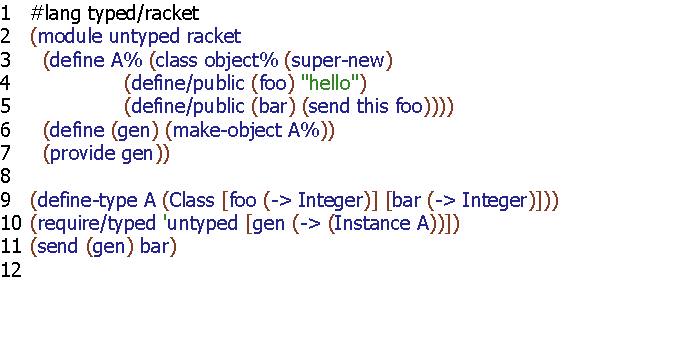
\includegraphics[scale=.7]{figures/internal.pdf}&\hspace{-2cm}
\begin{minipage}{.5\textwidth}
\vspace{-4.3cm}
\tiny
\begin{lstlisting}[basicstyle=\scriptsize\ttfamily]
foo: broke its own contract
  promised: Integer
  produced: "hello"
  in: the foo method in
      the range of
      (->
       (object/c
        (bar (-> any/c Integer))
        (foo (-> any/c Integer))))
  contract from: (interface for gen)
  contract on: gen
  blaming: (interface for gen)
\end{lstlisting}
\end{minipage}
\end{tabular}
\caption{Typed Racket ensures that internal untyped calls respect external types}
\label{fig:arktex3}
\end{figure}

To model this behavior in \kafka, we need to use a different approach to translation. 
At the most basic level, the simple naive translation approach, as seen in
figure~\ref{fig:rktex2}, would call the wrapped object, which would then call 
the \xt{foo} method without any type guards, and the program would 
only encounter a cast error once \xt{bar} returned.

We present an example in figure~\ref{fig:intbeh} to better illustrate this issue. The example describes a class \C
that is being forced to become class \D, which is typed in such a way that \C's
implementation of \n will violate the type guarantees imposed by \D and the wrapper \xt{DW}. 
Under the naive translation scheme, in figure~\ref{fig:intbeh}, the arguments to \m will be cast to \any, 
then passed into the untyped object. The untyped object \C will simply use its own definition
of the \m method, which calls directly into the \n method on that same object,
thereby circumventing the type applied to it by the type cast.

Interestingly, this property is not required for type soundness. Under this naive
translation, no type guarantee is broken, as the typed code never ``sees'' \n
violate the type contract. As a result, this naive translation is technically
sound, but does not accurately capture the semantics of Typed Racket.

\begin{figure}[!ht]
\begin{tabular}{l@{\hspace{0.05\textwidth}}l}
\begin{minipage}{0.34\textwidth}
\begin{lstlisting}
class A {n(x:*):*{x}}
class B {m(x:*):*{x}}
class C { 
  m(x:A):A { this.n(x) }
  n(x:A):A { x }}
class D { 
  m(x:A):A { new A() }
  n(x:B):B { new B()}}
(<D>new C()).m(new C())
\end{lstlisting}
\end{minipage} &
\begin{minipage}{0.6\textwidth}
\begin{lstlisting}
class DW {
  that : C


  m(x:A):A { this.that().m(x) }

  n(x:B):B { 
    (*@\hspace{-1.5mm}\BehStart\hspace{-1.5mm}@*)B(*@\BehEnd@*)(*@\ShaStart\hspace{-1.5mm}@*)B(*@\ShaEnd\hspace{0mm}@*)this.that().n((*@\hspace{-0.5mm}\BehStart\hspace{-1.5mm}@*)B(*@\BehEnd@*)(*@\ShaStart\hspace{-1.5mm}@*)B(*@\ShaEnd\hspace{0mm}@*)x) }
}
\end{lstlisting}
\end{minipage} \\
Example Program & Naive wrapper
\end{tabular}
\caption{Failing program and naive wrapper}
\label{fig:intbeh}
\end{figure}

To solve this problem, we have to guarantee that any self reference in the
underlying wrapped object will go through the wrapper. As we cannot do this
under the \kafka dynamics, we have to solve it in the way we generate the
wrapper classes.

We enforce the wrapper's type guarantee on the underlying object's methods by
lifting the body of the methods up into the wrapper, thereby making any self
reference in the underlying object trivially refer to the wrapper, illustrated 
in figure~\ref{fig:intbeh2}. However, this translation is still typed incorrectly, 
we are making an untyped call to a typed call site.


\begin{figure}[!ht]
\begin{tabular}{l@{\hspace{0.05\textwidth}}l}
\begin{minipage}{0.4\textwidth}
\begin{lstlisting}
class DW {
  that : C
  
  m(x:A):A { this.n(x) }
  n(x:B):B { 
    (*@\hspace{-1.5mm}\BehStart\hspace{-1.5mm}@*)B(*@\BehEnd@*)(*@\ShaStart\hspace{-1.5mm}@*)B(*@\ShaEnd\hspace{0mm}@*)(*@\hspace{-0.5mm}\BehStart\hspace{-1.5mm}@*)B(*@\BehEnd@*)(*@\ShaStart\hspace{-1.5mm}@*)B(*@\ShaEnd\hspace{0mm}@*)x }
}
\end{lstlisting}
\end{minipage} &
\begin{minipage}{0.55\textwidth}
\begin{lstlisting}
class DW {
  that : C
  m(x:A):A { 
    (*@\hspace{-0.5mm}\BehStart\hspace{-1.5mm}@*)A(*@\BehEnd@*)(*@\ShaStart\hspace{-1.5mm}@*)A(*@\ShaEnd\hspace{0mm}@*)this.n((*@\hspace{-0.5mm}\BehStart\hspace{-1.5mm}@*)B(*@\BehEnd@*)(*@\ShaStart\hspace{-1.5mm}@*)B(*@\ShaEnd\hspace{0mm}@*)x) }
  n(x:B):B { 
    (*@\hspace{-1.5mm}\BehStart\hspace{-1.5mm}@*)B(*@\BehEnd@*)(*@\ShaStart\hspace{-1.5mm}@*)B(*@\ShaEnd\hspace{0mm}@*)(*@\hspace{-0.5mm}\BehStart\hspace{-1.5mm}@*)B(*@\BehEnd@*)(*@\ShaStart\hspace{-1.5mm}@*)B(*@\ShaEnd\hspace{0mm}@*)x }
}
\end{lstlisting}
\end{minipage} \\
Type-incorrect wrapper & Type-corrected wrapper
\end{tabular}
\caption{Wrapper generation}
\label{fig:intbeh2}
\end{figure}

We overcome this issue through a special ``type-fixing'' operation, 
which ensures method bodies have the correct type 
once lifted into the wrapper. Finally, defining a behavioural cast semantics 
that preserves the execution behaviour of Typed Racket.

The corrected translation, on the right side of
figure~\ref{fig:intbeh2}, shows the correct behaviour of the wrapper, and
is both type correct and semantics-preserving. Notably, what we have
accomplished with the dynamic expression translation mechanism, in
section~\ref{behtrans}, is equivalent to the set of casts that would have occurred
if we had been able to insert the wrapper as the receiver for self references,
effectively in-lining the call through the wrapper.

Another challenge with Typed Racket is when multiple wrappers are layered 
over the target object. Each time a reference crosses a boundary between typed and untyped code,
it will accrue an additional wrapper. When a method is invoked on a wrapper
chain, that method will be invoked on every wrapper in the chain, until finding its way to
the target object. A key property of the wrapper generation functions, presented in section
\ref{wrap}, is that methods should not be ``lost''. That is to say, any method
in the target object, even if it is not in the type it is being cast to, will be
retained by the wrapper.  This property is somewhat unconventional, and it is 
illustrated in \figref{ctod} when executing the expression \BehCast\C{(\BehCast\D{\New\C{}})}. 
Class \C and \D are not related by subtyping as \any is not a supertype of \E. The inner cast from \C to
\D, results in the generation of class \EMxt{CtoD}. The wrapper class is a
subtype of \D but it also has method \mp only found in class \C.  The cast from
\EMxt{CtoD} back to \C leads to the generation of wrapper class \EMxt{CtoDtoC}.
The latter is a subtype of \C and has a rather interesting method \m which is
dynamic and thus must be invoked dynamically. The receiver is cast to \any using
a structural subtype cast. The argument on the other hand is converted to dynamic with a
behavioural cast. The return value is converted to the expected return type with
another behavioural cast.


%%%%%%%%%%%%%%%%% EXAMPLE  <C><D>new C %%%%%%%%%%%%%%%%%%%%%%%%%%%%%%%%%%%%
\begin{figure}
\footnotesize
\begin{tabular}{ll}\begin{minipage}{6cm}
\[\begin{array}{l}
\class ~\C~ \{\\
\SP  \Mdef\m\e\x\E\x\\
\SP  \Mdef\mp\e\x\E\x\\
\}\\[2mm]
\class ~\EMxt{CtoD}~ \{\\
\SP  \Fdef\that\C\\
\SP  \Mdef \m\x\any\any{\Call{\Get\this\that}\m{\BehCast\E\x}}\\
\SP  \Mdef \mp\e\x\E{\Call{\Get\this\that}\mp\x}\\
\}\\
\end{array}\]
\end{minipage}
&
\begin{minipage}{5cm}
\[\begin{array}{l}
\class ~\D~ \{\\
\SP  \Mdef\m\x\any\any\x\\
\}
\\
\\[2mm]
\class ~\EMxt{CtoDtoC}~ \{\\
\SP  \Fdef\that{\EMxt{CtoD}}\\
\SP  \Mdef\m\e\x\E{ \BehCast\E{\DynCall{(\SubCast\any{\Get\this\that})}\m{\BehCast\any\x}}}\\
\SP  \Mdef\mp\e\x\E{ \Call{\Get\this\that}\mp{\x}}\\
\}\\
\end{array}\]
\end{minipage}
\end{tabular}
\caption{Wrapper classes generated by \BehCast\C{(\BehCast\D{\New\C{}})}}
\label{ctod}
\end{figure}


%%%%%%%%%%%%%%%%%%%%%%%%%%%%%%%%%%%%%%%%%%%%%%%%%%%%%%%%%%%%%%%%%%%%%%%%


\section{Translation: Reticulated Python - Monotonic Semantics}

At the surface language level, the monotonic semantics and the transient 
semantics are very similar. Common to both semantics is the idea of 
consistency, which will become substantially more important in our 
discussion of the monotonic semantics. 

\begin{mathpar}
\IRule{C1}{\tmeet\t\tp\cdot\K = \tpp\,\Kp}{\consistent\K{\t}{\tp}} 
\end{mathpar}

Consistency is effectively the idea that two types \emph{do not
contradict one another}. For example, the types \xt{int} and \any are
consistent, but the types \xt{int} and \xt{string} are not as no member of
one could be in the other.

The consistency operator ($\sim$) in our formal system is implemented using the concept of meet described
by the \texttt{tmeet} function. The \xt{tmeet} function finds the common type 
between two given types, which if a common type exists, it implies that consistency holds between 
the two given types. Using the earlier example, the meet between \xt{int} and \any would be \xt{int}, 
as \xt{int} is the more restrictive of the two types. In effect, the \texttt{tmeet} function fulfills the 
same purpose as the $\sqcap$ operator in~\cite{Siek2015}. 

\begin{figure}[!ht]
\begin{tabular}{EEEEEVEV}
\texttt{tmeet(}
& \texttt{A}
  & \texttt{,}
  \texttt{B}
  & \texttt{,}
  $\cdot$
  & \texttt{,}
  &
\begin{lstlisting}
class A {
   m(x: *): A {this}}

class B {
   m(x: B): * {this}}
\end{lstlisting}    
& 
\texttt{) = C,}
  &
\begin{lstlisting}
class A { ... }
class B { ... }
class C {
  m(x: B): A {this}
}
\end{lstlisting}    
\end{tabular}
\caption{Simple example of \texttt{tmeet}}
\label{fig:tmeet_ex}
\end{figure}

Consider the simple example in figure~\ref{fig:tmeet_ex}, where we compute the meet of
\texttt{A} and \texttt{B}, both classes have the same function, but with alternating the typing. 
The function in class \texttt{A} has the return type typed, whereas the function in class \texttt{B} has the argument typed. 
Calling the \texttt{tmeet} function on \texttt{A} and \texttt{B} will compute the new type \texttt{C}, 
whose method have will have typed argument and return type. The \texttt{tmeet} function will be described 
in more detail later in this section, when the monotonic cast semantic is presented.


\begin{figure}[h!]
\begin{minipage}{0.35\textwidth}
\begin{mathpar}
\IRule{W10}{
  \EnvType \Env\s\K\e\tp
}{
  \EnvType \Env\s\K{\MonCast\t\e}\t
}
\end{mathpar}
\end{minipage}
\begin{minipage}{0.5\textwidth}
\begin{tabular}{l@{}l@{~}l@{~}l}
\CondRule{E11}{  %% Monotonic cast  
  \moncast \a\t\s\K  \Kp\ap\sp    
}{    
  \ReduceA  \K{\MonCast \t\a}\s \Kp\ap\sp   
} \\
\multicolumn{4}{l}{\EE ::= \ldots \B \MonCast\t\EE }
\end{tabular}
\end{minipage}
\caption{Monotonic cast static and dynamic rules}
\label{fig:monrules}
\end{figure}

Similar to the behavioural semantics, the monotonic semantics is implemented to the core of \kafka
as a cast extension. For an expression \e and type \t, we write \MonCast\t\a to depict the monotonic cast.
Figure \ref{fig:monrules} presents the typing and semantics rules for the monotonic cast.

\begin{figure}[!ht]
\newcommand{\monowrap}[2]{\xt{mwrap}(#1,#2)}
\begin{mathpar}
\IRule{PT}{
  {\classtrans{\K}{\K}{\K'}} \\ \GenCast{\K}{\cdot}{\e}{\ep}{\t} 
}{\progtrans{\e~\K}{\e'~{\K'}}}

\IRule{MCT1}{
  \D \text{ fresh}\\
  \k = \classgen{\C,\getmds\C\K,{\classoff\C\K},{\classoff\C\K},\D,\K}
}{
  \monowrap{\C}{\K} = \D~\k
}

\IRule{MCT2}{
}{
  \monowrap{\any}{\K} = \any
}

\IRule{CR1}{ 
  \b{\methtrans \K\C\md{\md'}{\K_m}} \\
  \classtrans \K\Kp\Kpp \\
  \b{\monowrap\t\Kpp = \tp~\Kppp}
}{
   \classtrans \K{\Class \C{\b{\Ftype\f\t}}{\b\md}~\Kp}{\Class \C {\b{\Ftype\f\tp}}{\b{\md'}}~\Kpp~\K_m~\b{\Kppp}}}

\IRule{CR2}{ 
}{
  \classtrans \K\cdot\cdot
}

\IRule{MT}{
  \AnaCastMono \K{\HT\this\C~\HT\x\t}\e\ep\tp{\K_1} \\
  \monowrap{\t_1}\K = \t_2~\K_2 \\
  \monowrap{\tp_1}\K = \tp_2~\K_3
}{
  \methtrans \K\C{\Mdef\m\x{\t_1}{\tp_1}\e}{\Mdef\m\x{\t_2}{\tp_2}\ep}{\K_1~\K_2~\K_3}
}
\end{mathpar}
\caption{Monotonic translation for program, class, and method}
\label{fig:mono-trans1}
\end{figure}


The translation from the monotonic surface language to \kafka begins 
in figure \ref{fig:mono-trans1}. The rule \RuleRef{PT} translates 
monotonic programs, \RuleRef{CR1} and \RuleRef{CR2} translates monotonic class,
and \RuleRef{MT} translates monotonic methods. In the \RuleRef{MT} 
and \RuleRef{CR1} rules, we are actively replacing every type the user wrote with ones generated by the 
\xt{monWrap} function. The details of the \xt{monWrap} function will be 
discussed later, but for the purposes of the translation, we can assume that the
\xt{monWrap} function will replace every typed function with an untyped one unless
there are no \any types transitively contained within the function's argument.

\begin{figure}[!ht]
\begin{mathpar}
\IRule{MOA1}{\HasType{\E}\x\t}{\GenCastMono{\K}\E\x\x\t{}}

\IRule[width=30em]{MOA2}{
    \GenCastMono\K\Env{\e_1}{\e_3}{\C}{\K_1} \\ \n(\b{\t_1}):\t_2 \in \classoff\C\K \\ \statictype{\t_1}{\K}{\cdot} \vee \n=\f \\ \b{\AnaCastMono\K\Env{\e_2}{\e_4}{\t_1}{\K_2}}
}{
    \GenCastMono\K\Env{\Call{\e_1}\n{\b{\e_2}}}{\Call{\e_3}\n{\b{\e_4}}}{\t_2}{\K_1~\b{\K_2}}
}

\IRule[width=30em]{MOA3}{
    \GenCastMono\K\Env{\e_1}{\e_3}{\C}{\K_1} \\ \m({\t_1}):\t_2 \in \classoff\C\K \\ \lnot\statictype{\t_1}{\K}{\cdot} \\ \b{\AnaCastMono\K\Env{\e_2}{\e_4}{\t_1}{\K_2}}
}{
    \GenCastMono\K\Env{\Call{\e_1}\m{{\e_2}}}{\DynCall{(\MonCast\any\e_3)}\m{\MonCast\any{\e_4}}}{\t_2}{\K_1~\b{\K_2}}
}

\IRule{MOA4}{
    \GenCastMono\K\Env{\e_1}{\e_3}{\any}{\K_1} \\ {\AnaCastMono\K\Env{\e_2}{\e_4}{\any}{\K_2}}
}{
    \GenCastMono\K\Env{\Call{\e_1}\m{{\e_2}}}{\DynCall{\e_3}\m{{\e_4}}}{\any}{\K_1~\K_2}
}

\IRule{MOA5}{
  \b{\AnaCastMono{\K}\E{\e_1}{\e_2}\t{\K}} \\ 
  \Class \C {\b{\Ftype\f\t}} {\b{\md}} \\
  \D~\text{fresh} \\
  \k = \classgen{\C,\getmds\C\K,\classoff\C\K,\classoff\C\K,\D,\K} \\
  }{\GenCastMono\K\Env{\New\C{\b{\e_1}}}{\New\D{\New\C{\b{\e_2}}}}{\C}{\K~\k}}
\end{mathpar}
\caption{Monotonic translation for expressions}
\label{fig:mono-trans2}
\end{figure}

The expression translations are presented in figure \ref{fig:mono-trans2}. 
The \texttt{static} function states whether a type contains only typed methods.
The rule \RuleRef{MOA2} translates typed methods, \RuleRef{MOA2} translate methods that are not purely typed.
\RuleRef{MOA4} translate untyped methods, \RuleRef{MOA2} translate object creation.
The purpose of the \xt{monWrap} function is further evidenced as the 
handling of calls to methods need to appropriately casted if the typing nature is unclear.

\begin{figure}[!ht]
\begin{mathpar}
\IRule{MOAASC1}{
  \GenCastMono\K\Env\e\ep\tp\K \\
  \K \vdash \tp \Sub \t
}{
  \AnaCastMono\K\Env\e\ep\t\K
}

\IRule{MOAASC2}{
  \GenCastMono\K\Env\e\ep\tp\K \\
  \consistent\K\t\tp
}{
  \AnaCastMono\K\Env\e{\MonCast\t\ep}\t\K
}
\end{mathpar}

\caption{Monotonic translation for bidirectional expressions}
\label{fig:mono-trans3}
\end{figure}

The bidirectional nature of the monotonic translation require the two 
expression translation rules, \RuleRef{MOAASC1} and \RuleRef{MOAASC2}, 
in figure \ref{fig:mono-trans3}.

\subsection{Monotonic Casts}

The monotonic cast \MonCast\C\a imposes the type \C onto the object
at \a and every object transitively reachable from \a. The motivation 
for this cast comes from~\cite{Siek2015}, where it is used to maintain the
type correctness of every reference in the program.

\begin{figure}[h!]
\begin{tabular}{ll}
\begin{minipage}[b]{4cm}
\lstset{framesep=4pt}
\begin{lstlisting}
class C { f : * }
class D { 
  m (x:*):* {x}
}

d:* = new D()
a:* = new C(d)
[heap snapshot 1]

class E { f : F }
class F { 
  m (x:E):E {x}
}

e:E = <E>a
[heap snapshot 2]
d.m(d)
\end{lstlisting}
\vspace{-9.2em}
\end{minipage}
&
\begin{tabular}{l}
\\
Heap snapshot 1: \\
\begin{minipage}{8cm}
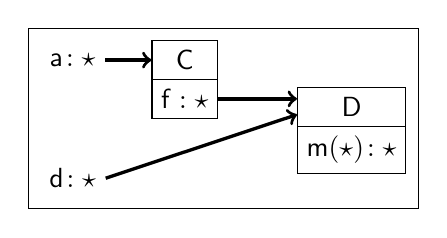
\begin{tikzpicture}[framed,my shape/.style={
rectangle split, rectangle split parts=#1, draw, anchor=text east}]
\node (ref) at (0,0) {$\HT\a\any$};
\node (refb) at (0,-1.5) {$\HT{\xt{d}}\any$};

\node (C1) [my shape=2,right of=ref, anchor = text west]
{\C\nodepart{two}$\f : \any$};

\node (D1) [my shape=2,right=of C1.two east, anchor=text west,shift={(0,-.1)}]
{\D\nodepart{two}$\Mtype\m\any\any$};

\draw[->,very thick] (ref.east) -> (C1.text west);
\draw[->,very thick] (refb.east) -> ($(D1.text west)+(0,-.1)$);
\draw[->,very thick] (C1.two east) -> ($(D1.text west)+(0,.1)$);
\end{tikzpicture}
\end{minipage}\\
\\
Heap snapshot 2: \\
\begin{minipage}{8cm}
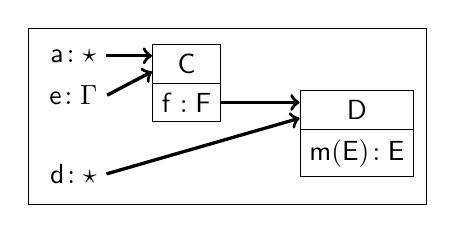
\begin{tikzpicture}[framed,my shape/.style={
rectangle split, rectangle split parts=#1, draw, anchor=text east}]
\node (ref) at (0,0) {$\HT\a\any$};
\node (refb) at (0,-1.5) {$\HT{\xt{d}}\any$};
\node (refe) at (0,-.5) {$\HT{\xt{e}}\E$};

\node (C1) [my shape=2,right of=ref, anchor = text west,shift={(0,-.1)}]
{\C\nodepart{two}$\f : \xt{F}$};

\node (D1) [my shape=2,right=of C1.two east, anchor=text west,shift={(0,-.1)}]
{\D\nodepart{two}$\Mtype\m{\xt{E}}{\xt{E}}$};

\draw[->,very thick] (ref.east) -> ($(C1.text west)+(0,.1)$);
\draw[->,very thick] (refb.east) -> ($(D1.text west)+(0,-.1)$);
\draw[->,very thick] (refe.east) -> ($(C1.text west)+(0,-.1)$);
\draw[->,very thick] (C1.two east) -> ($(D1.text west)+(0,.1)$);
\end{tikzpicture}
\end{minipage}
\end{tabular}
\vspace{1em}
\end{tabular}
\caption{Execution under the monotonic semantics}
\label{fig:mono_ex1}
\end{figure}

Figure~\ref{fig:mono_ex1} illustrates the semantics of the monotonic cast. 
A new instance of class \D is created and then an instance of class \C 
is created pointing to it. At this point, as shown by heap snapshot 1, 
the field \f on \C has type \any, and the method \m on \D has fully dynamic 
argument and return type. Next we introduce classes \E and \xt{F}, which are structurally 
identical to \C and \D, but have specific types for their fields and methods. 
If the instance of class \C in the program, referenced by \a, is casted to \E, 
the monotonic semantics will ensure any access to field \f or method \m from 
anywhere in the program will follow the type invariants asserted by class \E.

However, as shown in heap snapshot 2, the variable \xt{d} still refers to 
the instance of \D, from earlier in the program, and \xt{d}
does not know the existence of the new invariants applied to class \D. Despite being
typed \any, when \xt{d} try to invoke method \m on the apparently dynamic 
object, a cast failure will occur. The monotonic semantics ensures that the
provided argument is of type \E. 

This example highlights the need for the monotonic cast semantics to be generative.
In order to guarantee the type correctness of all references, monotonic has to generate guards
that check the argument and return type of every method, and the
type of any field set, ensuring that they maintain consistency with the 
maximally static type. Additionally, since monotonic has to ensure that 
prior references respect future type invariants, it has to do in-place updates
of any object whose type is altered by a cast update.

In the extreme case, a single cast could cause every object in the heap to be
retyped. To prevent pathological cases, the monotonic casts only modify the heap
if the target \C has fewer occurrences of \any than the original type of the
object at \a (and transitively so for types appearing in \t and reachable
from \a).  When a type \C does not have any occurrence of the dynamic type,
denoted by \statictype\C\K\V, the monotonic casts will leave the object and the
heap unchanged.

A key challenge is for every reference in the heap \s to still be valid after a monotonic
cast. If a reference has a type other than \any, then the cast will preserve correctness of that
reference. To accomplish this, the cast ensure two properties hold:
\begin{itemize}
\item The values that currently exist cannot violate any of the types
  that point to them. Casting needs to recursively ensure that all values
  referred to by the current object are of the claimed type.
\item Functions can not be called with or return values that violate any of
  the types that they are referred to. The behaviour of the class needs
  to check that its types are not violated by lesser-typed call sites.
\end{itemize}
The second property is strongly reminiscent of the behavioural semantics,
though with the interesting caveat that all method invocations 
must follow the typed calling conventions, rather
than just the ones that inherit this particular type assertion.

The monotonic cast semantics in \kafka cannot be implemented using the simple 
in-place replacement technique\cite{Siek2015}. In order to ensure the
type of a field is respected, the monotonic cast will have to insert a setter method
that checks the value it is given against the type of the field, when
a lesser-typed call site is used to set the field. However, \kafka prohibits
the explicit existence of a field and its getter and setter methods, 
as a consequence of having uniform treatment for fields and their getter and setter methods. 

This treatment of fields means the monotonic cast semantics is implemented by adding a 
single wrapper over each object, similar to the ``identity preserving membrane''
described in \cite{keil_et_al:DARTS:2015:5511}. The wrappers will preserve the
externally-facing interface (up to a point) and the relations between classes,
while ensuring all properties in the monotonic system are guaranteed.

As a result of generating the wrappers (and the static translation), the simple example 
shown in figure~\ref{fig:mono_ex1} does not correctly exhibit the behavior of the 
monotonic cast semantics in \kafka. The monotonic cast semantics of \kafka are
depicted by the example presented in figure~\ref{fig:mono_ex2}.
For compactness, the class definitions in figure~\ref{fig:mono_ex1}, and the class definitions that will be generated but
not appear in the dynamic execution have been elide.

\begin{figure}[h!]
\centering
\begin{minipage}{5cm}
\begin{tabular}{l}
Translated Program:\\
\begin{lstlisting}
d:* = new DW(new D())
a:* = new CW(new C(d))
[heap snapshot 1]
e:E = <E>a
[heap snapshot 2]
d.m(d)
\end{lstlisting}
\end{tabular}
\end{minipage}
\begin{tabular}{@{}l@{\hspace{3mm}}l@{}}
Class \C Wrappers: & Class \D Wrappers: \\
\begin{minipage}{7cm}
\begin{lstlisting}
class CW { 
    that : C
    f():* { <*>this.that().f() }
    f(x:*):* { 
      <*>this.that().f(<*>x)}
}
class ECW {
  that : C
  f():* { <*><FW>this.that.f() }
  f(x:*):* {
      <*><F>this.that().f(<*><FW>x)}
}
\end{lstlisting}
\end{minipage}
&
\begin{minipage}{7cm}
\begin{lstlisting}
class DW { 
  that : D
  m (x:*):* { <*><*>x }
}



class FDW {
  that : D
  m(x:*):* { <*><EW><*><EW>x }
  m(x:E):E { <EW><*><EW>x }
}
\end{lstlisting}
\end{minipage}
\\
Heap snapshot 1: & 
Heap snapshot 2: \\
\begin{minipage}{7cm}
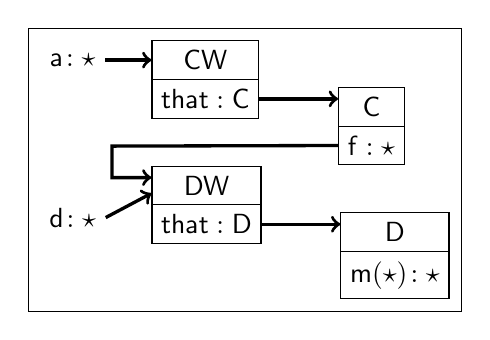
\begin{tikzpicture}[framed,my shape/.style={
rectangle split, rectangle split parts=#1, draw, anchor=text east}]
\node (ref) at (0,0) {$\HT\a\any$};
\node (refb) at (0,-2) {$\HT{\xt{d}}\any$};

\node (C1) [my shape=2,right of=ref, anchor = text west]
{\xt{CW}\nodepart{two}$\that : \C$};

\node (C2) [my shape=2,right=of C1.two east, anchor=text west,shift={(0,-.1)}]
{\xt{C}\nodepart{two}$\f : \any$};

\node (D1) [my shape=2,below=of C1.two west, anchor=text west,shift={(0,-.1)}]
{\xt{DW}\nodepart{two}$\that : \D$};

\node (D2) [my shape=2,right=of D1.two east, anchor=text west,shift={(0,-.1)}]
{\xt{D}\nodepart{two}$\Mtype\m\any\any$};

\draw[->,very thick] (ref.east) -> (C1.text west);
\draw[->,very thick] (refb.east) -> ($(D1.text west)+(0,-.1)$);
\draw[->,very thick] (C1.two east) -> ($(C2.text west)+(0,.1)$);
\draw[->,very thick] (C2.two west) -- ($(D1.text west) + (-0.5,0.5)$) -- ($(D1.text west) + (-0.5,.1)$) -> ($(D1.text west)+(0,.1)$);
\draw[->,very thick] (D1.two east) -> ($(D2.text west) + (0,.1)$);
\end{tikzpicture}
\end{minipage} &
\begin{minipage}{7cm}
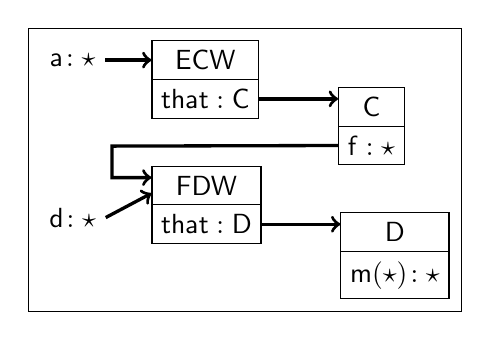
\begin{tikzpicture}[framed,my shape/.style={
rectangle split, rectangle split parts=#1, draw, anchor=text east}]
\node (ref) at (0,0) {$\HT\a\any$};
\node (refb) at (0,-2) {$\HT{\xt{d}}\any$};

\node (C1) [my shape=2,right of=ref, anchor = text west]
{\xt{ECW}\nodepart{two}$\that : \C$};

\node (C2) [my shape=2,right=of C1.two east, anchor=text west,shift={(0,-.1)}]
{\xt{C}\nodepart{two}$\f : \any$};

\node (D1) [my shape=2,below=of C1.two west, anchor=text west,shift={(0,-.1)}]
{\xt{FDW}\nodepart{two}$\that : \D$};

\node (D2) [my shape=2,right=of D1.two east, anchor=text west,shift={(0,-.1)}]
{\xt{D}\nodepart{two}$\Mtype\m\any\any$};

\draw[->,very thick] (ref.east) -> (C1.text west);
\draw[->,very thick] (refb.east) -> ($(D1.text west)+(0,-.1)$);
\draw[->,very thick] (C1.two east) -> ($(C2.text west)+(0,.1)$);
\draw[->,very thick] (C2.two west) -- ($(D1.text west) + (-0.5,0.5)$) -- ($(D1.text west) + (-0.5,.1)$) -> ($(D1.text west)+(0,.1)$);
\draw[->,very thick] (D1.two east) -> ($(D2.text west) + (0,.1)$);
\end{tikzpicture}
\end{minipage}
\end{tabular}
\caption{Execution under the monotonic semantics}
\label{fig:mono_ex2}
\end{figure}

Figure~\ref{fig:mono_ex2} aims to illustrate the nature of the monotonic wrappers. 
In this example, the state of the heap is highlighted
at two discrete times, before and after the cast of the reference \a to
the type \xt{E}. The wrapper \xt{CW} and \xt{DW} is associated with enforcing 
the class \C and \D, respectively, and wrap over an underlying object of 
known type, enforcing its type guarantees.

The monotonic semantics will lift method bodies into wrapper classes, as seen in
the Typed Racket semantics but for different reasons. While Typed Racket
needs to enforce the observed type on an underlying untyped object. The
monotonic semantics need the combination of the wrapper and underlying object 
to act as if they are exactly the monotonically specified type. 
The result of this can be seen in the translation above for \m.

A notable behavior of the monotonic semantics illustrated in figure~\ref{fig:mono_ex2}
is the erasure on every call site for \m, with the exception of the final definition in \xt{FDW}. 
Under the monotonic semantics, every call site with some untyped component somewhere
will be adjusted further, ensuring any partially typed call may be invalidated in the future. 
As a consequence, every call, even to a superficially typed call site (one with an argument
type that may contain a \any deeply embedded in the type), must be treated as an untyped call site.

In the monotonic semantics, if we encounter a cast on a reference, that cast needs to be
enforced upon that reference for the rest of its lifetime. \kafka's monotonic
cast semantics handles this by taking the previously-existing type on the object,
computing the meet of that old type and the new type, producing a new
wrapper for the object that replaces the previous wrapper. The wrappers \xt{ECW} and \xt{FDW}
are created when \a is casted to \xt{E}.
To ensure that types for fields are respected, we take a conservative approach, 
as seen in \xt{ECW}. When a field on an underlying object is set, we first cast
it to the required type (in this case \xt{FW}). Then a further $\star$ cast is applied 
to the type of the underlying storage cell. For retrieving values, we reverse this process.

The result wrappers are sometimes overly conservative. From the semantics of the meet operation, we
know that the first cast to the protected type is sufficient to ensure 
compatibility with the underlying memory cell type, and we also know that casting
to the required type before returning is ignoring the heap consistency invariant 
that monotonic provides, allowing for casts on retrieval to be ignored. However,
the \kafka type system does not allow us to make either of these shortcuts while
still retaining semantic correctness, and as a result, we are forced to double 
up casts on the getter and setter methods, as seen in \xt{ECW}.
Another point of interest is the alteration happening in \xt{FDW}. When the class \xt{D}
is specialized to \xt{F}, a lot of additional (and, in this case, not necessary) casts
are inserted, as well as a wholly new call site for \m. This new
call site is fully typed, despite previously stating that we could not add any 
typed call sites as they might be changed in the future.
In this case, we are able to insert the additional static call site because we 
know that \xt{E} will not be able to be further altered under the monotonic 
semantics, as \xt{E} and every type referenced from it have no instances of the
type \any in them, which might be altered in the future by another monotonic
cast.

\begin{figure}
\begin{mathpar}
\IRule{CM}{
  \retype \a\t\cdot\s\K = \S~\Kp\\
  \spec {\Dom\S} \S\s\Kp = \sp~\Kpp
}{
  \moncast \a\t\s\K \Kpp \sp\\
}
\end{mathpar}
\caption{Monotonic cast semantics}
\label{fig:mono_sem}
\end{figure}

The monotonic cast semantics is formally defined by the \xt{moncast} rule, 
which takes the address of the cast object \a, a target type \t, the current heap \s, 
and class table \K, and gives an update heap \sp and an updated class table \Kp.

The functionality of the \xt{moncast} rule is broken into two functions.
The first function (\xt{retype}) identities the correct target type for every object affect by
the monotonic cast, storing the gathered objects and their types in the meta-variable \S, 
a mapping from addresses to classes, creating a blueprint for the sub-heap affected 
by the monotonic cast. The second function (\xt{spec}) updates the heap and class table with the
objects and types listed in \S.

\begin{figure}[!ht]
\opdef{
  $\tmeet{\t}{\tp}\P\K = \tpp\,\Kp$
}{
}
\begin{align*}
\P &::= \cdot \B \Map\P{\Bind{(\C,\D)}\E}
\end{align*}
\begin{mathpar}
\IRule{TM1}{ }{\tmeet\C\any\P\K = \C\,\K}

\IRule{TM2}{ }{\tmeet\any\C\P\K = \C\,\K}

\IRule{TM3}{ }{\tmeet\t\t\P\K = \t\,\K}

\IRule{TM4}{
  \fresh\E\\
  (\C,\D) \not\in\P \\
  \Pp = \Map\P{\Bind{(\C,\D)}\E} \\
  \mtypes\C\K = {\b\mt}\\
  \mtypes\D\K = {\b\mtp}\\
  \mmeet{\b\mt}{\b\mtp}\Pp\K = \b\mtpp\,\Kp\\
  \Kpp = \Kp~\typegen{\b\mtpp}\E\\
}{
    \tmeet\C\D\P\K = \E\,\Kpp
}

\IRule{TM5}{
    \P(\C,\D) = \E
}{
    \tmeet\C\D\P\K = \E\,\K
}
\end{mathpar}
\caption{The \texttt{tmeet} function}
\label{fig:tmeet_fun}
\end{figure}

The \xt{retype} function utilizes the meet operation in determining the correct
casting type for every object transitively reachable from the cast object. 
Figure~\ref{fig:tmeet_fun} presents the \xt{tmeet} function, which computes
the meet between two types. The \xt{tmeet} function takes four arguments,
the two types being meet, a meta-variable \P, and the class table \K. 
The meta-variable \P denotes a list of mappings 
from a pair of types to the type produced from their meet. The rules
\RuleRef{TM1} and \RuleRef{TM2} describe the meet of a $\star$. The rule
\RuleRef{TM3} describes the identity meet. The rule \RuleRef{TM5} describes
the recursive case of our meet operation. 
The rule \RuleRef{TM4} retrieves the method typing for each type, computes 
the meet of those method typing (by calling an auxiliary function (\xt{mmeet}),
and updates the class table with a new class containing the method typing 
produced from the meet.

\begin{figure}[!ht]
\begin{tabular}{l@{}l@{}l@{}l@{}l@{\hspace{1.5mm}}l@{\hspace{1mm}}l@{}l}
\texttt{tmeet(}
& \texttt{A}
  & \texttt{,}
  \texttt{B}
  & \texttt{,}
  $\cdot$
  & \texttt{,}
  &
  \begin{minipage}{4.3cm}
    \begin{lstlisting}
class A {
   m(x: A): A {this}}

class B {
   m(x: B): B {this}}
      \end{lstlisting}    
  \end{minipage}
& 
\texttt{) = E,}
  &
  \begin{minipage}{4.3cm}
    \begin{lstlisting}
class A { ... }
class B { ... }
class E {
  m(x: E): E {this}
}
    \end{lstlisting}    
  \end{minipage}
\end{tabular}
\caption{\texttt{tmeet} example over recursive classes}
\label{fig:tmeet_rec_ex}
\end{figure}

The meta-variable \P becomes crucial when considering the example
in figure~\ref{fig:tmeet_rec_ex}, where the meet  of \xt{A} and \xt{B}
recursively depends on the meet of \xt{A} and \xt{B}. If we proceeded naively,
without \P, \RuleRef{TM4} would invoke \RuleRef{TM4} again to compute the meet
of the arguments to \m. We use \P and \RuleRef{TM5} to avoid this.

\RuleRef{TM4} invokes \xt{mmeet} with an enriched \P, in much the same manner
that the subtyping relation does, inserting the future result of the meet of
\xt{A} and \xt{B} (\xt{E} in this example) into \P, will then
be used by \RuleRef{TM5} to terminate the recursion.

\section{Conclusion}

Gradual typing is no longer simply a popular research topic in academia.
Real world applications are being written with gradual typing like languages.
Types are progressively being introduced into existing untyped applications.
It's the responsibility of language researchers to present a clear understanding 
of each viable gradual typing idiom available.

We have presented \kafka, a formal language that serves as the foundation for 
constructing five existing gradual typing systems: Typescript, Thorn, Transient, 
Type Racket, and Monotonic. \kafka offers the opportunity for comparing and 
contrasting these gradual typing systems within an unified framework. The translations
to \kafka for each gradual typing system highlights the essences which makes each system unique.

From \kafka, we have developed a better understanding for the lightweight nature of TypeScript,
the restrictiveness of Thorn, the excessiveness of the wrappers generated by Type Racket,
the safety guarantees of Transient, and the complexity and dynamic nature of Monotonic.
However, the aim of this paper is not only to provide a deeper understanding for each
individual gradual typing system, but a road map for the direction of gradual typing in general.

In the future, we intend on exploring the possibility of mixing and matching the varies 
cast semantics within \kafka. In particular, the interaction between the behavioural cast semantics 
and the Monotonic cast semantics should be considered worth exploring.
The decision to describe the Monotonic cast semantics via wrapper generation was influenced
by the existence of the getter and setter methods necessary for the behavioural cast semantic.
It would be worthwhile to consider designing a system similar to \kafka using the in place 
replacement technique. 


\clearpage

\bibliographystyle{unsrturl}
\bibliography{../bib/jv,../bib/all,../bib/ben}

\appendix
%%%%%%%%%%%%%%%%%%%%%%%%%%%%%%%%%%%%%%%%%%%%%%%%%%%%%%%%%%%%%%%%%%%%%%%%%%%%%%
%%%%%%%%%%%%%%%%%%%%%%%%%%%%%%%%%%%%%%%%%%%%%%%%%%%%%%%%%%%%%%%%%%%%%%%%%%%%%%
\section{Auxiliary Definitions for \kafka}%%%%%%%%%%%%%%%%%%%%%%%%%%%%%%%%%%%%
%%%%%%%%%%%%%%%%%%%%%%%%%%%%%%%%%%%%%%%%%%%%%%%%%%%%%%%%%%%%%%%%%%%%%%%%%%%%%%
%%%%%%%%%%%%%%%%%%%%%%%%%%%%%%%%%%%%%%%%%%%%%%%%%%%%%%%%%%%%%%%%%%%%%%%%%%%%%%

\subsection{Subtyping}

The structural subtype relation, written \StrSub\M\K\t\tp, asserts that \t
is a subtype of \tp in the environment composed of a set of subtyping \M and
a class table \K.   The set of subtypings can be omitted if empty.

~\\

\opdef{\StrSub\M\K\t\tp}{\t is a subtype of \tp}
\begin{mathpar}
\IRule{SRef}{
}{
 \StrSub\M\K \t \t
}

\IRule{SAss}{
\C \Sub \D \in \M
}{
 \StrSub \M\K \C \D
}

\IRule{SRec}{
 \M' = \M~\C\Sub\D\\
\mt \in \classoff\D\K \implies \mtp \in \classoff\C\K ~.~ \StrSub{\M'}\K\mt{\mtp}
}{
 \StrSub \M\K \C \D 
}
\end{mathpar}

\begin{mathpar}
\IRule{SMet}{
  \StrSub \M\K {\t[1]} {\t[2]} \\
  \StrSub \M\K {\tp[2]} {\tp[1]}
}{
 \StrSub \M\K {\Mtype\m{\t[1]}{\tp[1]}} {\Mtype\m{\t[2]}{\tp[2]}}
}

\IRule{SGet}{
  \StrSub \M\K {\t[1]} {\t[2]}
}{
 \StrSub \M\K {\Mtype\f{}{\t[1]}} {\Mtype\f{}{\t[2]}}
}

\IRule{SSet}{
  \StrSub \M\K {\t[1]} {\t[2]}
}{
 \StrSub \M\K {\Mtype\f{\t[1]}{\t[1]}} {\Mtype\f{\t[2]}{\t[2]}}
}
% \IRule{SThat}{
% }{
%   \StrSub\M\K{\Mtype\that{\b{\t[1]}}{\t[1]}}{\mt}
% }
\end{mathpar}

\subsection{Well-formedness}

The overloading function is meant to check that every typed method is
defined once. Every untyped method is defined once. A class has either a
field \f or a pair of getter and setters. \\

\opdef{~\WFp\e\K}{Well-formed program}

\begin{mathpar}
\IRule{WP}{
  \k \in \K \implies \WF{}\cdot\K\k \\
  \EnvType\Env\cdot\K\e\t
}{
  \WFp\e\K
}
\end{mathpar}

\opdef{\WF{}\s\K {\Class\C{\b\fd}{\b\md}}}{Well-formed class}

\begin{mathpar}
\IRule{WC}{
 \xt{overloading}(\b\fd,\b\md)\OK \\
 \fd\in\b\fd\implies \WF {\text{this}:\C~}\s\K \fd \\
 \md\in\b\md\implies \WF {\text{this}:\C~}\s\K \md 
}{
 \WF {}\s\K {\Class \C {\b\fd}{\b\md}}
}
\end{mathpar}

The \xt{overloading} auxiliary function states that there are no overloaded 
field or method names within the given field and method definitions. \\

\opdef{~\WF \Env\s\K \md}{Well-formed methods}
\begin{mathpar}
\IRule[width=18em]{WT}{
 \EnvType {\Env{~\Ftype\x\C}~}\s\K\e\D\\
 \WFtype\K\C \\
 \WFtype\K\D \\
}{
 \WF \Env\s\K {\Mdef\m\x\C\D\e}
}

\IRule[width=18em]{WU}{
 \EnvType {\Env~\Ftype\x\any~}\s\K \e\any\\
}{
 \WF \Env\s\K{\Mdef\m\x\any\any\e}
}

\IRule{WS}{
 \EnvType {\Env{~\Ftype\x\tp}~}\s\K \e\t \\
 \WFtype \K\t 
}{
 \WF  \Env\s\K {\Mdef\f\x\t\t\e}
}

\IRule{WG}{
 \EnvType \Env\s\K\e\t \\
 \WFtype \K\t
}{
 \WF \Env\s\K {\Mdefz\f\t\e}
}
\end{mathpar}

\opdef{~\WF  \Env\s\K {\Fdef\f\t}}{Well-formed fields}
\begin{mathpar}
\IRule{WF}{
 \WFtype \K\t 
}{
 \WF  \Env\s\K {\Fdef\f\t}
}
\end{mathpar}

\opdef{~\WFtype\K\t}{Well-formed types}
\begin{mathpar}
\IRule{WA}{
}{
 \WFtype\K\any
}

\IRule{WC}{
 \C \in \K
}{
 \WFtype\K\C
}
\end{mathpar}

\subsection{Expression typing}

Field accessor rules W3 and W4 require a typed receiver, since \any does
not have any methods a receiver typed at \any will never typecheck.

Shallow casts, W9, do not change the type of the expression. We are casting
to the name of \t not to \t.  In practice that means that all expression
types in Transient will drift towards \any.

~\\

\opdef{\EnvType\Env\s\K\e\t}{\e has type \t in environment \Env against heap \s and class table \K}
\begin{mathpar}

\IRule{W1}{
   \HasType \Env\x\t
 }{
   \EnvType \Env\s\K\x\t
}

\IRule{W2}{
 }{
   \EnvType \Env\s\K\a\any
}

\IRule{W3}{
  \EnvType \Env\s\K\e\tp \\
 \StrSub \M\K \tp \t
 }{
  \EnvType \Env\s\K\e\t 
}   

\IRule{W4}{
  \EnvType \Env\s\K\e\C \\
  \Mtype \f{}\tp \in \classoff\C\K
}{
  \EnvType \Env\s\K{\Get\e\f}\tp
}    

\IRule{W5}{
  \EnvType \Env\s\K\e\C \\
  \Mtype \f\tp\tp \in \classoff\C\K  \\
  \EnvType \Env\s\K\ep\tp
}{
  \EnvType \Env\s\K{\Set\e\f\ep}\tp
}    

\IRule{W6}{
  \EnvType \Env\s\K\e\C \\
  \Mtype \m\tp\tpp\in \classoff\C\K  \\
  \EnvType \Env\s\K\ep\tp
}{
  \EnvType \Env\s\K{\Call\e\m\ep}\tpp
}    

\IRule{W7}{
  \EnvType \Env\s\K\e\any \\
  \EnvType \Env\s\K\ep\any
}{
  \EnvType \Env\s\K{\DynCall\e\m\ep}\any
}    

\IRule{W8}{
 \EnvType \Env\s\K{\e_1}{\t_1}\dots 
 \EnvType \Env\s\K{\e_n}{\t_n}\ \\ 
 \b\fd=\Fdef{\f_1}{\t_1}\dots\Fdef{\f_n}{\t_n} \\ 
  \Class \C {\b\fd}{\b\md} \in \K
}{
  \EnvType \Env\s\K{\New\C{\e_1\dots\e_n}}\C
}

\IRule{W9}{
  \EnvType \Env\s\K\e\tp
}{
  \EnvType \Env\s\K{\SubCast\t\e}\t
}

\IRule{W10}{
  \EnvType \Env\s\K\e\tp
}{
  \EnvType \Env\s\K{\ShaCast\t\e}\any  %%!!!  not \t !!!
}

% \IRule{W11}{
%   \EnvType \Env\s\K\e\tp
% }{
%   \EnvType \Env\s\K{\MonCast\t\e}\t
% }

\IRule{W11}{
  \s(\a) = \obj\C{\b\ap}
}{
  \EnvType \Env\s\K\a\C
}

\IRule{W12}{
  \Env(\text{this}) = \D \\
  \Class \D {\text{that}:\C}{...} \in\,\K \\
}{
  \EnvType \Env\s\K{\Get{\text{this}}{\text{that}}}\C
}

\IRule{W13}{
  \Env(\text{this}) = \D \\
  \Class \D {\text{that}:\C}{...} \in\,\K\\
  \EnvType \Env\s\K\e\C \\
}{
  \EnvType \Env\s\K{\Set{\text{this}}{\text{that}}\e}\C
}
\end{mathpar}


\subsection{Field read}

We write \readf\s\a\f\K to denote a read of field \f from the object
stored at \a in \s.

\begin{equation*}
\readf \s\a\f\K = \ap 
  ~~\mathit{if}~~ \begin{cases}  \s(\a) = \obj\C{\a_1\dots\a_n \ap \dots}\\
 \Class\C {\Fdef{\f_1}{\t_1}\dots\Fdef{\f_n}{\t_n}\Ftype\f\t\dots}{\b\md}\in\K
 \end{cases}
\end{equation*}

\subsection{Write field}

We write \setf\s\a\f\ap\K to denote the write of value \ap into field \f of
the object stored at \a in \s.

\begin{equation*}
\setf \s\a\f\ap\K= \Map\s{\Bind{\a}{\obj\C{\a_1\dots\a_n\,\ap\dots}}}
  ~~\mathit{if}~~ \begin{cases}
   \s(\a) = \obj\C{\a_1\dots\a_n\,\app\dots}\\
   \Class\C{\Fdef{\f_1}{\t_1}\dots\Fdef{\f_n}{\t_n}\,\Fdef\f\t\dots}{\b\md}\in\K
\end{cases}
\end{equation*}

% \clearpage

\section{Generative Behavioural Casts}

\subsection{Expression translation for Behavioural semantics}\label{behtrans}

% \begin{figure}[!ht]
% \hrulefill
\begin{mathpar}
\IRule{REW1}{ }{ \rtranst{\b{\mt}}{\b{\mtp}}\e\x\x{[\e/\x]\x} }

\IRule{REW2}{ \x \neq \x' }{ \rtranst{\b{\mt}}{\b{\mtp}}\e\x{\x'}{\x'} }
\\
\IRule[width=25em]{REW3}{ \Mtype\n{\b{\t_1}}{\tp_1} \in \b{\mt} \\ \Mtype\n{\b{\t_2}}{\tp_2} \in \b{\mtp} \\ \n = \f \vee \tp[2] \neq \any  \\ 
\b{\rtranst{\b{\mt}}{\b{\mtp}}\e\x{\e}{\ep}}}{\rtranst{\b{\mt}}{\b{\mtp}}\e\x{\Call{\this}\n{\b\e}}{\BehCast{\tp_1}{\Call{\this}\n{\b{\BehCast{\t_2}{\ep}}}}}}
\\
\IRule[width=18em]{REW4}{ \Mtype\m{{\t_1}}{\tp_1} \in \b{\mt} \\ \Mtype\m{{\any}}{\any} \in \b{\mtp} \\ 
\b{\rtranst{\b{\mt}}{\b{\mtp}}\e\x{\e}{\ep}}}{\rtranst{\b{\mt}}{\b{\mtp}}\e\x{\Call{\this}\m{\e}}{\BehCast{\tp_1}{\DynCall{\this}\m{{\BehCast{\any}{\ep}}}}}}

\IRule[width=25em]{REW5}{ \Mtype\n{\b{\t_1}}{\tp_1} \in \b{\mt} \\ \Mtype\n{\b{\t_2}}{\tp_2} \not\in \b{\mtp}  \\ 
\b{\rtranst{\b{\mt}}{\b{\mtp}}\e\x{\e}{\ep}}}{\rtranst{\b{\mt}}{\b{\mtp}}\e\x{\Call{\this}\n{\b\e}}{{\Call{\this}\n{\b{{\ep}}}}}}

\IRule[width=20em]{REW6}{ \e_1 \neq \this \\ \rtranst{\b{\mt}}{\b{\mtp}}\e\x{\e_1}{\e_2} \\ \b{\rtranst{\b{\mt}}{\b{\mtp}}\e\x{\ep_1}{\ep_2}}}{\rtranst{\b{\mt}}{\b{\mtp}}\e\x{\Call{\e_1}\n{\b{\ep_1}}}{\Call{\e_2}\n{\b{\ep_2}}}}

\IRule{REW7}{ \rtranst{\b{\mt}}{\b{\mtp}}\e\x{\e_1}{\e_2} \\ \rtranst{\b{\mt}}{\b{\mtp}}\e\x{\ep_1}{\ep_2}}{\rtranst{\b{\mt}}{\b{\mtp}}\e\x{\DynCall{\e_1}\m{\ep_1}}{\DynCall{\e_2}\m{\ep_2}}}

\IRule{REW8}{ \b{\rtranst{\b{\mt}}{\b{\mtp}}\e\x{\e}{\ep}} }{\rtranst{\b\mt}{\b\mtp}\e\x{\New\C{\b\e}}{\New\C{\b\ep}}}
\end{mathpar}

% \vspace{-2mm}
% %%%%%%%%%%%%%%%%%%%%%%%%%%%%%%%%%%%%%%%%%%%%%%%%%%%%%%%%%%%%%%%%%%%%%%%%%%%%%
% \hrulefill
% \caption{Behavioral dynamic expression translation.}\label{behtrans}
% \end{figure}

% \clearpage

\subsection{Class wrapper for Behavioural semantics}\label{wrap}

% TODO: FIX the formatting.

% \begin{figure}[!ht]
% \hrulefill 
\scriptsize
\newcommand{\bscast}[2]{\EM{\BehCast{#1}{\ShaCast{#1}{#2}}}}
\vspace{4mm}
%%%%%%%%%%%%%%%%%%%%%% WRAP %%%%%%%%%%%%%%%%%%%%%%%%%%%%%%%%%%%%%%%%%%%%%%%%%
%\IGNOREUNLESSNEEDED{
\[\begin{array}{@{}ll@{}l@{}r@{~}c@{~}r}
    \wrap\C{\b\md}\bmt\bmtp\D = \\
\SP \class ~\D ~ \{\\
\SPP \Fdef\that\C \\
\SPP \Mdefz\f{\tp}{~\bscast\tp{\Get{\Get\this\that}\f}~}
&    \Mtype\f{}\t\in\bmt &\wedge& \Mtype\f{}\tp \in \bmtp
\\
\SPP \Mdef\f\x\tp\tp {~\bscast\tp{\Set{\Get\this\that}\f{\bscast\t\x}}~}
&    \Mtype\f\t\t \in \bmt &\wedge& \Mtype\f\tp\tp \in \bmtp
\\
\SPP \Mdef\m\x\t\tp {~\bscast\tp{{\ep}}~}
&     \All \m \Mdef\m\x\Cp\Cpp\e\in\b\md &\wedge& \Mtype\m\t\tp\in\bmtp \\
&\multicolumn{5}{l}{~\wedge~\rtranst{\bmt}\bmtp{(\bscast\Cp\x)}\x{\e}{\ep}}
\\
\SPP \Mdef\m\x\any\any {~\SubCast\any{\Call\this\m{\bscast{\t}\x}}~}
&     \All \m \Mdef\m\x\Cp\Cpp\e\in\b\md &\wedge& \Mtype\m\t\tp\in\bmtp\\
&\multicolumn{5}{l}{~\wedge~\Mdef\m\x\any\any{\e'}\not\in\b\md}
\\
\SPP \Mdef\m\x\t\tp{~\bscast\tp{\ep}~}
&    \All \m \Mdef\m\x\any\any\e\in\b\md &\wedge& \Mtype\m\t\tp\in\bmtp \\
&\multicolumn{5}{l}{~\wedge~\rtranst{\bmt}\bmtp{(\bscast\any\x)}\x\e{\ep}}
\\
\SPP \Mdefz\f\t { ~\Get{\Get\this\that}\f~}
&    \Mtype\f{}\t \in \bmt &\wedge& \Mtype\f{}\tp \not\in \bmtp
\\
\SPP \Mdef\f\x\t\t { ~\Set{\Get\this\that}\f\x~}
&    \Mtype\f\t\t \in \bmt&\wedge& \Mtype\f\tp\tp \not\in \bmtp
\\
\SPP \Mdef\m\x{\Cp}{\Cpp} {~\ep~}
&    \All \m  \Mdef\m\x\Cp\Cpp\e\in\b\md &\wedge& \Mtype\m\t\tp\not\in \bmtp \\
&\multicolumn{5}{l}{~\wedge~\rtranst{\bmt}\bmtp\x\x{\e}{\ep}}
\\
\SPP \Mdef\m\x\any\any {~\ep~}
&    \All \m  \Mdef\m\x\any\any\e\in\b\md  &\wedge& \Mtype\m\t\tp\not\in\bmtp \\
&\multicolumn{5}{l}{~\wedge~\rtranst{\bmt}\bmtp\x\x{\e}{\ep}}
\\
\SP \}
\\
\wrapAny\C\bmd\bmt\D = \\
\SP \class~\D~\{\\
\SPP \Fdef \that \C\\ 
\SPP   \Mdefz\f\any{~\BehCast\any{\Get{{\Get\this\that}}\f}~}
&  \Mtype\f{}\t \in \bmt\\
\SPP   \Mdef\f\x\any\any{~\BehCast\any{\Set{\Get\this\that}\f{\bscast\t\x}}~}
&  \Mtype\f\t\t \in \bmt\\
\SPP   \Mdef\m\x\any\any {~\BehCast\any{{\ep}}~}
&  \All \m \Mdef\m\x\t\t\e\in\b\md \\
&\multicolumn{5}{l}{~\wedge~\rtranst{\bmt}{\dyn{\bmt}}{(\BehCast\t\x)}\x{\e}{\ep}}
\\
\SP \}\\
\end{array}\]
%}%%END IGNORE
%   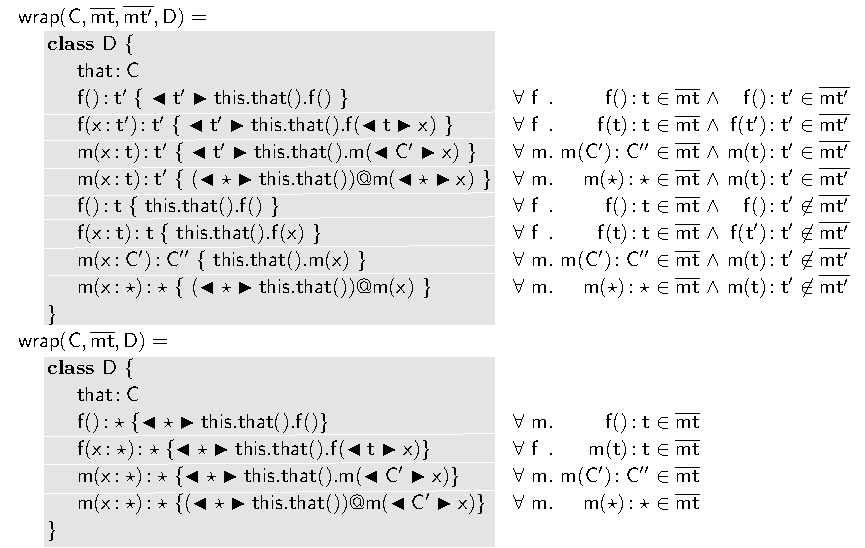
\includegraphics[width=.9\textwidth]{figures/wrapDefinition}
% TODO: untyped(mt)
% \hrulefill
% %%%%%%%%%%%%%%%%%%%%%%%%%% WRAP %%%%%%%%%%%%%%%%%%%%%%%%%%%%%%%%%%%%%%%%%%%%%%%
%   \caption{Wrapper class generation.}\label{wrap}
% \end{figure}

% \clearpage

\normalsize

\section{Generative Monotone Casts}

\subsection{Retype function}\label{retype}

Formally, the \xt{retype} function takes a list of object
addresses \b\a and a list of types to ascribe to them \b\t, and updates the
heap \s and class table \K. 

\begin{mathpar}
\IRule{CRM1}{
  \htype \a\S\s\K = \C~\Kp\\
  \tmeet\C\t\cdot\Kp = \D\,\Kpp\\ 
  \C\not\EQ\D  \\
  \ftypes \a\D \s\Kpp = \b\ap~\b\tp \\
  \Sp = \Map\S{\Bind\a\D } \\
  \retype{\b\ap}{\b\tp}\Sp\s\K = \Spp\,\K'''
}{
  \retype \a\t\S\s\K = \Spp\,\K'''
}

\IRule{CRM2}{
  \htype \a\S\s\K = \tp\,\Kp\\
  \tmeet\tp\t\cdot\Kp = \tpp\,\Kp \\
  \tp\EQ\tpp \\
}{
  \retype \a\t\S\s\K = \S~\Kpp
}

\IRule{CRM3}{
  \retype\a\t\S\s\K = \Sp\,\Kp\\
  \retype{\b\a}{\b\t}\Sp\s\Kp = \Spp\,\Kpp
}{
  \retype {\a\,\b\a}{\t\,\b\t}\S\s\K = \Spp\,\Kpp
}
\end{mathpar}

\subsection{Spec function}\label{mono:spec}

Formally, the \xt{spec} (heap specialization) function takes a
sequence of object addresses \b\a, a heap typing \S, a heap \s
and a class table \K and returns a new heap where the objects
have been retyped. \Dom\S retrieves the list of addresses 
that have to be retyped.

\begin{mathpar}
\IRule{CMS1}{
  \E \text{ fresh}\\
  \D = \App\S\a \\
  \obj\C{\ap} = \App\s\a \\
  \obj\Cp{\b\app} = \App\s\ap \\
  \classoff\Cp\Kpp = \b\mt \\
  \classoff\D\Kpp = \b\mtp \\  
  \names{\b\mtp} \subseteq \names{\b\mt}\\
  \Kp = \K~\classgen{\Cp,\b\mt,\b\mtp,\E,\K} \\
  \sp = \Map\s{\Bind\a{\E\{\ap\}}}
}{
  \spec \a\S\s\K = \sp~\Kp
}

\IRule{CMS2}{
  \spec \a\S\s\K = \sp\\
  \spec {\b\a}\S\sp\K =\spp
}{
   \spec {\a\,\b\a}\S\s\K = \spp
}
\end{mathpar}

\subsection{Meet function}\label{monmeet}

The \texttt{mmeet} function is used by the \texttt{tmeet} functions to
perform the meet over the typing of each method within a class definition.
The \texttt{mmeet} function also takes four arguments, the method
signatures of the original class $\b\mt$, the method signatures of the cast
class $\b\mtp$, the environment $\P$, a class table $\K$, and outputs method
types $\b\mtpp$ and a class table $\Kp$. \\

% \hrulefill

\opdef{
  $\mmeet{\b\mt}{\b\mtp}\P\K = \b\mtpp\,\Kp$
}{
}
\begin{mathpar}
\IRule{MM1}{
}{
  \mmeet{\b\mt}{\cdot}\P\K =\b{\mt} ~\K
}

\IRule{MM2}{
}{
  \mmeet{\cdot}{\b\mt}\P\K =\b{\mt} ~\K
}

\IRule{MM3}{ 
  \Mtype\f{}{\t} = \mt \\
  \Mtype\f{}{\tp} \in \b{\mtp} \\
  \tmeet{\t}{\tp}\P\K = \tpp~\Kp \\
  \Mtype\f{}{\tpp} = \mtpp
}{ 
   \mmeet{\mt}{\b{\mtp}}\P\K = \mtpp\,\Kp
}

\IRule{MM4}{ 
  \Mtype\f{\t}{\t} = \mt \\
  \Mtype\f{\tp}{\tp} \in \b{\mtp} \\
  \tmeet{\t}{\tp}\P\K = \tpp~\Kp \\
  \Mtype\f{\tpp}{\tpp} = \mtpp
}{ 
   \mmeet{\mt}{\b{\mtp}}\P\K = \mtpp\,\Kp
}


\IRule{MM5}{ 
  \Mtype\m{\t_1}{\t_2} = \mt \\
  \Mtype\m{\t_3}{\t_4} \in \b{\mtp} \\
  \tmeet{\t_3}{\t_1}\P\K = \t_5~\Kp \\
  \tmeet{\t_2}{\t_4}\P\Kp = {\t_6}~{\Kpp} \\
  \Mtype\n{\t_5}{\t_6} = \mtpp
}{ 
   \mmeet{\mt}{\b{\mtp}}\P\K = \mtpp\,\Kpp 
}

\IRule{MM6}{
  \mmeet{\mt}{\b{\mt_2}}\P\K = \mt_3~\Kp\\
  \mmeet{\b{\mt_1}}{\b{\mt_2}}\P\Kp = \b{\mt_4}~\Kpp
}{
  \mmeet{\mt~\b{\mt_1}}{\b{\mt_2}}\P\K =\mt_3\b{\mt_4} ~\Kpp
}
\end{mathpar}
\\

\subsection{Monotonic dynamic expression translation}\label{montrans}


\begin{mathpar}
\IRule{MREW1}{ }{ \rtranstz{\b{\mt}}{\b{\mtp}}\x\x }
\\
\IRule[width=25em]{MREW2}{ 
  \Mtype\n{\b{\t_1}}{\tp_1} \in \b{\mt} \\ 
  \Mtype\n{\b{\t_2}}{\tp_2} \in \b{\mtp} \\ 
  \n = \f \vee \t_2 \neq \any  \\ 
  \b{\rtranstz{\b{\mt}}{\b{\mtp}}{\e}{\ep}}
}{
  \rtranstz{\b{\mt}}{\b{\mtp}}{\Call{\this}\n{\b\e}}{\MonCast{\tp_1}{\Call{\this}\n{\b{\MonCast{\t_2}{\ep}}}}}
}
\\

\IRule[width=20em]{MREW3}{ 
  \Mtype\n{\b{\t_1}}{\tp_1} \in \b{\mt} \\ 
  \Mtype\n{\b{\t_2}}{\tp_2} \not\in \b{\mtp} \\ 
  \b{\rtranstz{\b{\mt}}{\b{\mtp}}{\e}{\ep}}
}{
  \rtranstz{\b{\mt}}{\b{\mtp}}{\Call{\this}\n{\b\e}}{{\Call{\this}\n{\b{{\ep}}}}}
}

\IRule[width=20em]{MREW4}{ 
  \e_1 \neq \this \\ \rtranstz{\b{\mt}}{\b{\mtp}}{\e_1}{\e_2} \\ 
  \b{\rtranstz{\b{\mt}}{\b{\mtp}}{\ep_1}{\ep_2}}
}{
  \rtranstz{\b{\mt}}{\b{\mtp}}{\Call{\e_1}\n{\b{\ep_1}}}{\Call{\e_2}\n{\b{\ep_2}}}
}

\IRule{MREW5}{ 
  \rtranstz{\b{\mt}}{\b{\mtp}}{\e_1}{\e_2} \\ 	
  \rtranstz{\b{\mt}}{\b{\mtp}}{\ep_1}{\ep_2}
}{
  \rtranstz{\b{\mt}}{\b{\mtp}}{\DynCall{\e_1}\m{\ep_1}}{\DynCall{\e_2}\m{\ep_2}}
}

\IRule{MREW6}{
  \b{\rtranstz{\b{\mt}}{\b{\mtp}}{\e}{\ep}} 
}{
  \rtranstz{\b\mt}{\b\mtp}{\New\C{\b\e}}{\New\C{\b\ep}}
}
\end{mathpar}


\subsection{Monotonic class generation}\label{classgen}

\footnotesize
\[\begin{array}{l@{~}r@{}r@{~}r@{~}r@{~}rr}
\arrayrulecolor{white}
\classgen{\C, \b\md, \bmt, \bmtp, \D, \K}= \\
\SP \class~\D~\{ \\
\SPP \Fdef\that\C
\\[1mm]
\SPP \Mdef\f\x\any\any {\SubCast\any{\MonCast\tp{
      \Set{\Get\this\that}\f{\MonCast\t{\MonCast\tp\x}}}}}
&
\All f \Mtype\f\t\t\in\bmt &\wedge& \Mtype\f\tp\tp\in\bmtp
\\[1mm]\hline
\SPP \Mdefz\f\any{\SubCast\any{\MonCast\tp{\Get{\Get\this\that}\f}}}
&
 \All f \Mtype\f{}\t \in \bmt &\wedge& \Mtype\f{}\tp \in \bmtp
\\[1mm]\hline
\SPP \Mdef\m\x\any\any {~\SubCast\any{\MonCast{\tp[2]}{{[{(\MonCast{\t[1]}\x)}/\x]\ep}}}~}
&     \All \m \Mdef\m\x{\t[1]}{\tp[1]}\e\in\b\md &\wedge& \Mtype\m{\t[2]}{\tp[2]}\in\bmtp \\
&&\wedge&\multicolumn{3}{l}{\rtranstz{\bmt}\bmtp{[{(\MonCast\t\x)}/\x]\e}{\ep}}
\\[1mm]\hline
\SPP \Mdef\m\x{\t[2]}{\tp[2]} {\MonCast{\tp[2]}{[{(\MonCast{\t[1]}\x)}/\x]\ep}~}
&     \All \m \Mdef\m\x{\t[1]}{\tp[1]}\e\in\b\md &\wedge& \Mtype\m{\t[2]}{\tp[2]}\in\bmtp \\
&&\wedge&\multicolumn{3}{l}{\rtranstz{\bmt}\bmtp{\e}{\ep}} \\
&&\wedge&\multicolumn{3}{l}{\statictype{\t[2]}{\K}{\cdot}}
\\[1mm]\hline
\SP\}
\end{array}
\]
\normalsize





\subsection{Monotonic equivalent type generation}\label{typegen}

\footnotesize
\[\begin{array}{l@{~}r@{}r@{~}r@{~}r@{~}rr}
\arrayrulecolor{white}
\typegen{\bmt}{\D} = \\
\SP \class~\D~\{
\\[1mm]
\SPP \Mdef\m\x\t\tp {{\MonCast\tp{\x}}} 
&
\All m \Mtype\m\t\tp\in\bmt
\\[1mm]\hline
\SPP \Mdef\f\x\t\t {\x}
&
\All f \Mtype\f\t\t\in\bmt
\\[1mm]\hline
\SPP \Mdefz\f\t{{\MonCast\t{\New\D{}}}}
&
 \All f \Mtype\f{}\t \in \bmt
\\[1mm]
\SP\}
\end{array}
\]
\normalsize




\subsection{Htype function}

The function \htype\a\S\s\K
returns the class of the object at address \a.  \htype\a\S\s\K is \C if \C =
\App\S\a or if $\a\not\in\S$ and \obj\C{\b\a}=\App\s\a.

\begin{mathpar}
\IRule{HT1}{
  \a \not\in \text{addr}(\S) \\
  \enfortype\C\cdot\K = \D\,\W\,\Kp
}{
  \htype\a\S{\sigma[\a \mapsto \C\{\ap\}]}\K = \D~\Kp
}

\IRule{HT2}{
  \S(\a) = \t
}{
  \htype{\a}{\S}{\sigma}\K = \t~\K
}
\end{mathpar}

\subsection{Lifting function}

% \hrulefill
\begin{align*}
\W &::= \cdot \B \Map\W{\Bind\C\D}
\end{align*}
\begin{mathpar}
\IRule{ENT1}{ 
  \Class\C{\hspace{-0.3em}}{\Fdef\that\Cp ~ \b\md} \in \K \\ 
  \C \notin \text{dom}(\W) \\
  \D\text{ fresh} \\
  \Wp = \W\,\Bind\C\D \\
  \Kp = \K\,\Class\D{\hspace{-0.3em}}{\Fdef\that\Cp ~ \enformt{\b{\md}}{\Wp}{\K}} \\ 
}{
  \enfortype{\C}{\W}{\K} = \D\,\Wp\,\Kp
}

\IRule{ENT2}{ 
  \W(\C) = \D \\
}{
  \enfortype{\C}{\W}{\K} = \D\,\W\,\K
}

\IRule{ENT3}{ 
}{
  \enfortype{\any}{\W}{\K} = \any\,\W\,\K
}
\end{mathpar}
\\

% \hrulefill

\begin{mathpar}
\IRule{ENMT1}{
  \md =  \Mdef\m\x\any\any {~\SubCast\any{\MonCast\tp{{[{(\MonCast\t\x)}/\x]\ep}}}~} \\
  \enfortype\t\W\K = \tpp\,\Wp\,\Kp \\
  \enfortype\tp\Wp\Kp = \tppp\,\Wpp\Kpp \\
  \mdpp = \Mdef\m\x\tpp\tppp {\MonCast\tppp\x} \\
  \enformt{\b\md}{\Wpp}{\Kpp} = \b\mddp \\
}{
  \enformt{\md\,\b\md}{\W}{\K} = \mdpp\,\b\mddp
}

\IRule{ENMT2}{
  \md = \Mdef\m\x\t\tp {\ep~}\\ 
  \enfortype\t\W\K = \tpp\,\Wp\,\Kp \\
  \enfortype\tp\Wp\Kp = \tppp\,\Wpp\Kpp \\  
  \mdpp =\Mdef\m\x\tpp\tppp {\MonCast\tppp\x}\\
  \enformt{\b\md}{\Wpp}{\Kpp} = \b\mddp \\
}{
  \enformt{\md\,\b\md}{\W}{\K} = \mdpp\,\b\mddp
}

\IRule{ENFS}{
  \md = \Mdef\f\x\any\any {\SubCast\any{\MonCast\tp{\Set{\Get\this\that}\f{\MonCast\t{\MonCast\tp\x}}}}} \\ 
  \enfortype\t\W\K = \tpp\,\Wp\,\Kp \\
  \enfortype\tp\Wp\Kp = \tppp\,\Wpp\Kpp \\   
  \mdpp = \Mdef\f\x\tpp\tppp {\MonCast\tppp\x} \\
  \enformt{\b\md}{\Wpp}{\Kpp} = \b\mddp \\
}{
  \enformt{\md\,\b\md}{\W}{\K} = \mdpp\,\b\mddp
}

\IRule{ENFG}{
  \md =  \Mdefz\f\any{\SubCast\any{\MonCast\t{\Get{\Get\this\that}\f}}} \\ 
  \enfortype\t\W\K = \tp\,\Wp\,\Kp \\
  \mdpp = \Mdefz\f\tp {\MonCast\tp{\Get{\Get\this\that}\f}} \\
  \enformt{\b\md}{\Wp}{\Kp} = \b\mddp \\
}{
  \enformt{\md\,\b\md}{\W}{\K} = \mdpp\,\b\mddp
}

\IRule{ENE}{
}{
  \enformt{\cdot}{\W}{\K} = \cdot
}
\end{mathpar}

\subsection{Static function}

\opdef{
  $\statictype\D\K{\b\C} = \texttt{Bool}$
}{
}

\begin{mathpar}
\IRule{ST1}{ 
}{ 
  \statictype\any\K{\b\C} = \texttt{False} 
}

\IRule{ST2}{ 
 \D \in {\b\C}
}{ 
  \statictype\D\K{\b\C} = \texttt{True} 
}

\IRule{ST3}{
  \D ~\text{empty}
}{ 
  \statictype\D\K{\b\C} = \texttt{True} 
}

\IRule{ST4}{
 \Class \C {\b{\Ftype\f\t}}{\b\md} \in \K \\
 \sign{\b\md} = \b{\Mtype\m\tp\tpp} \\ 
 \b\Cp = \b\C, \D
}{ 
  \statictype\D\K{\b\C} = \statictype{\b\t}\K{\b\Cp} \cap \statictype{\b\tp}\K{\b\Cp} \cap \statictype{\b\tpp}\K{\b\Cp}
}
\end{mathpar}
\\

\subsection{Wftype function}

\wftype{\b\f}\C\K denotes the function that looks up the type of a particular set of fields in \C.

\begin{equation*}
\wftype{\b\f}\C\K = \b\t ~~\mathit{if}~~ \begin{cases}

 \Class \C {\b{\Ftype\fp\tp}}{\b\md} \in \K\\
 \b\t = \{ \b\t \subseteq \b\tp ~|~ \forall~ \f \in \b\f ~.~ \f \in \names{\b{\Ftype\fp\tp}} \} \\
 
\end{cases}
\end{equation*}

\subsection{Mtype function}

The \texttt{mtypes} function takes a class name $\C$ and the class table
$\K$, and outputs a list of typing signatures $\b\mt$ for every method in
class $\C$, which includes the implicit getter and setter methods for every
field in the definition of class $\C$.  (\textbf{Note}: An user cannot
define a getter or setter method for any field that already exists in the
class. Similarly, a field cannot be declared in a class that already has a
getter or setter method for that field. This is enforced by the
\texttt{overloading} function in class well-formedness.)

\begin{equation*}
\classoff\C\K = \b\mt ~~\mathit{if}~~ \begin{cases}

 \Class \C {\b{\Ftype\f\t}}{\b\md} \in \K\\
 \b\mt = \sign{\b\md} \oplus \forall ~\Ftype\f\t \in \b{\Ftype\f\t} ~|~ \f \notin \names{\b\md} ~\wedge~ \f\neq\that ~.~ \typez{\Ftype\f\t}

\end{cases}
\end{equation*}

\subsection{getmds function}

$\getmds(\C,\K)$ denotes the function that returns the method definitions inside the class \C.

\begin{equation*}
\getmds\C\K = \b\md ~~\mathit{if}~~ \Class\C{\b{\fd}}{\b\md} \in \K
\end{equation*}

\subsection{Ftype function}

The function \ftypes\a\C\s\K returns the old references and the new types
for them according to the new wrapper \C.

\begin{mathpar}
\IRule{FT1}{
 \App\s\a=\obj\D{\ap} \\ % we know that a refers to a wrapper with a that field of the wrapped object
  \App\s\ap =\obj\E{\b\app}  \\ % getting the fields out of ap
 \Class \E {\b{\Fdef\f\t}}{\b\md} \in\K \\
 \wftype{\b\f}\C\K =\b\tp
}{
  \ftypes \a\C\s\K = \b\app~\b\tp
}
\end{mathpar}


\subsection{Dynamic function}

\begin{mathpar}
\IRule{DYN1}{
 \dyn{\b\mt} = \b{\mtp} \\
}{
  \dyn{\Mtype{\m}{\t}{\t} ~\,\b\mt} = \Mtype{\m}{\any}{\any}~\,\b\mtp
}

\IRule{DYN2}{
 \dyn{\b\mt} = \b{\mtp} \\
}{
  \dyn{\Mtype{\f}{\t}{\t} ~\,\b\mt} = \Mtype{\f}{\any}{\any}~\,\b\mtp
}

\IRule{DYN3}{
 \dyn{\b\mt} = \b{\mtp} \\
}{
  \dyn{\Mtype{\f}{}{\t} ~\,\b\mt} = \Mtype{\f}{}{\any}~\,\b\mtp
}

\IRule{DYNE}{
}{
  \dyn{\cdot} = \cdot
}
\end{mathpar}

\subsection{Signature function}

\begin{mathpar}
\IRule{SGE}{
}{
  \sign{\cdot} = \cdot
}

\IRule{SG1}{
  \md = \Mdef\m\x\t\t\e \\
  \sign{\b\md} = \b\mt \\
}{
  \sign{\md\,\b\md} = \Mtype\m\t\t~~\b\mt
}

\IRule{SG2}{
  \md = \Mdef\f\x\t\t\e \\
  \sign{\b\md} = \b\mt \\
}{
  \sign{\md\,\b\md} = \Mtype\f\t\t~~\b\mt
}

\IRule{SG3}{
  \md = \Mdefz\f\t\e \\ 
  \sign{\b\md} = \b\mt \\
}{
  \sign{\md\,\b\md} = \Mtype\f{}\t~~\b\mt
}
\end{mathpar}

\subsection{Typing function}

\begin{mathpar}
\IRule{TY1}{
}{
  \typez{\Ftype\f\t} = \Mtype\f\t\t~~\Mtype\f{}\t
}
\end{mathpar}

% \section{Monotonic figure scratch}

%% Example -- please check

%%class A {
%%  m(x:*):* { x }  
%%}
%% a = new A()
%% a.m(new A()) -- works fine
%%class B {
%%  m(x:B):B { x }  
%%}
%% b = <|B|> a
%% b.m(new B()) -- works
%% a.m(new A()) -- fails

% translated version

%%class wA {
%%  that : A
%%  m(x:*):* { this.that().m(x) }
%%}
%%a = new wA(new A())
%%(<*>a)@(<*>new wA(new A()))
%%class AmB {
%%  m(x:B):B{ ... }
%%}
%%class AwAmB {
%%  that : A
%%  m(x:*):* { <|*|><|B|>(<|*|>this.that())@m(<|*|><|B|>x) }
%%  m(x:B):B { <|B|>(<|*|>this.that())@m(<|*|>x)}  
%%}
%% b = <|B|> a -- b and a instance of AwAmB
%% b.m(new B()) -- works
%% a.m(new A()) -- fails

% example 2

%% class T { }
%% class A { f : * }
%% class B { f : A }
%% class C { f : B }
%% a1 = new A(new T())
%% a2 = new A(a1)
%% a3 = new A(a2)
%% b = <|B|> a3
%% c = <|C|> a3

% translated

%% class WA { that : A f():* { <|*|><|*|> this.that().f() } f(x:*):* { <|*|><|*|> this.that().f(<|*|><|*|>s x)} }
%% class WAmB { that:A f():* { <|*|><|A|>this.that().f() } f(x:*):* {<|*|><|A|> this.that().f(<|*|><|A|> x) } }
%% class WAmBmC { that:A f():* {<|*|> <|B|> this.that().f() } f(x:*):* { <|*|> <|B|> this.that().f(<|*|><|B|> x)} }
%% a1 = new WA(new A(new WT(new T())))
%% a2 = new WA(new A(a1))
%% a3 = new WA(new A(a2))
%% b = <|B|> a3 -- s(b) : WAmB
%% a3.f(new T()) -- boom
%% a2.f(new T()) -- ok
%% c = <|C|> b -- s(b) : WAmBmC, s(a2) : WAmB
%% a3.f(new T()) -- boom
%% a3.f(new WA(new A(new T))) -- boom
%% a2.f(new T()) -- boom

%% class A {
%%   fa : B
%%   ma(x : A): B { fa.mb(a) }
%% }
%% class B {
%%   fb : any
%%   mb(x:A):B { this }
%% }
%% class C {}

%% class Ap {
%%   fa : Bp
%%   ma(x : Ap): Bp {...}
%% }
%% class Bp {
%%   fb: C 
%%   ma(x : Ap): Bp {...}
%% }

%% a = new A(new B(new C()))
%% ap = <| Ap |> a

%% class WA {
%%   that : A
%%   fa() : B { that.fa() }
%%   fa(x:B):B { that.fa(x) }
%%   ma(x:B):B { that.ma(x) }
%% }
%% class WB {
%%   that : any
%%   fb() : any { that.fb() }
%%   fb(x:any):any { that.fb(x) }
%%   mb(x:B):B { that.mb(x) }
%% }
%% class WBp {
%%   that : A
%%   ...


\section{Proofs of Related Theorems}
\subsection{Accessory Lemmas}

\paragraph{Evaluation Extends Class Tables}

If $\Reduce \K\e\s \Kp\ep\sp$ then $\Kp = \K~\Kpp$ for some $\Kpp$.

\paragraph{Weakening of Subtyping}

If $\StrSub\cdot\K\t\tp$ then $\StrSub\cdot{\K~\Kp}\t\tp$.

\paragraph{Correctness of \classoff{\C}{\K}}

If $\Mtype\n{\b\t}\tp \in \classoff{\C}{\K}$, $\EnvType\cdot\s\K\e\C$ and (if applicable) $\EnvType\cdot\s\K\ep\t$, then $\Reduce \K{\Call\e\n{\b\ep}}\s \K\epp\s$ where $\EnvType\cdot\s\K\epp\tp$

\subsection{Soundness of \kafka Typing}

Given that $\WFp\K\e\s$ and $\EnvType\cdot\s\K\e\t$, then either there is some $\ep$ such that $\Reduce \K\e\s \Kp\ep\sp$ and $\WFp\Kp\ep\sp$ and $\EnvType\cdot\sp\Kp\ep\t$ hold, or $\e$ is of one of the following forms:
\begin{itemize} 
\item $\a$
\item $\DynCall\ep\m{\epp}$
\item $\SubCast\tp\ep$
\item $\ShaCast\tp\ep$
\item $\BehCast\tp\ep$
\item $\MonCast\tp\ep $
\end{itemize}
We proceed with rule induction on the judgement used to conclude $\EnvType\Env\s\K\e\t$. Note that we refer to rule preconditions from left to right.
\begin{itemize}
  \item W1

        Not applicable, since $\Gamma = \cdot$ and therefore contains no variables.
  \item W2

        We apply the IH to the first precondition. If we get stuck in the IH, then the entire expression gets stuck or terminates, trivially. Therefore, the interesting case is when $\Reduce \K\e\s \Kp\ep\sp$, $\WFp\Kp\ep\sp$ and $\EnvType\cdot\sp\Kp\ep\tp$. By 
  \item W3, W4, W5
  \item W6
  \item W7
  \item W8
  \item W9
  \item W10
  \item W11
  \item W12
\end{itemize}

\subsection{Type Correctness of Translation}


\end{document}

%######## ##    ## ########      #######  ########    ########   #######   ######  ##     ## ##     ## ######## ##    ## ######## 
%##       ###   ## ##     ##    ##     ## ##          ##     ## ##     ## ##    ## ##     ## ###   ### ##       ###   ##    ##    
%##       ####  ## ##     ##    ##     ## ##          ##     ## ##     ## ##       ##     ## #### #### ##       ####  ##    ##    
%######   ## ## ## ##     ##    ##     ## ######      ##     ## ##     ## ##       ##     ## ## ### ## ######   ## ## ##    ##    
%##       ##  #### ##     ##    ##     ## ##          ##     ## ##     ## ##       ##     ## ##     ## ##       ##  ####    ##    
%##       ##   ### ##     ##    ##     ## ##          ##     ## ##     ## ##    ## ##     ## ##     ## ##       ##   ###    ##    
%######## ##    ## ########      #######  ##          ########   #######   ######   #######  ##     ## ######## ##    ##    ##    




\subsection{others}

%TODO Fix ME \mtype\m\C\K = \convert{\methz\m\C\K} 

\hrulefill

\opdef{\classoff\C\K}{Auxiliary function: Type definition}

\begin{equation*}
\classoff\C\K = \EMxt{MT} ~~s.t.~~ \begin{cases}

 \K(\C) = \Class \C {\b{\Ftype\f\t}}{\b\md} \\
 \EMxt{MT} = \{\convert{\b\md} \oplus \forall ~\Ftype\fp\tp \in \b{\Ftype\f\t} ~|~ \fp \notin \b{\names{\md}} ~.~ \convertFD{\Ftype\fp\tp}\}

\end{cases}
\end{equation*}

\hrulefill


\opdef{\classoffs\a\s\K}{Auxiliary function: Type definition}

\begin{equation*}
\classoffs\a\s\K = \EMxt{MT} ~~s.t.~~ \begin{cases}

 \s(\a) = \obj\C{\b\a} \\
 \K(\C) = \Class \C {\b{\Ftype\f\t}}{\b\md} \\
 \EMxt{MT} = \{\convert{\b\md} \oplus \forall ~\Ftype\fp\tp \in \b{\Ftype\f\t} ~|~ \fp \notin \b{\names{\md}} ~.~ \convertFD{\Ftype\fp\tp}\}

\end{cases}
\end{equation*}

\hrulefill

\opdef{\ftype\f\C\K}{Auxiliary function: Field type lookup}

\begin{equation*}
\ftype\f\C\K = \t ~~s.t.~~ \begin{cases}

 \K(\C) = \Class \C {\ldots ~ \Ftype\f\t ~ \ldots}{\b\md}
\end{cases}
\end{equation*}

\hrulefill

\opdef{\field\C\K}{Auxiliary function: Field definition}

\begin{equation*}
\field\C\K = \b{\Ftype\f\t} ~~s.t.~~ \begin{cases}

 \K(\C) = \Class \C {\b{\Ftype\f\t}}{\b\md}
\end{cases}
\end{equation*}




This common core is focused on the basics of object functionality, with a
simple example being a \xt{Point} class.\footnote{For our examples we use
  integers and common arithmetic operations even if they are not in core
  calculus.}

%%% FIXME: formatting
\begin{verbatim}
class Point {
  x : Int
  y : Int
  addx( v : Int ) : Int {
       this.x!( this.x() + v )
  }
  addy( v : Int ) : Int {
       this.y!( this.y() + v )
  }
}
\end{verbatim}

The type system ensures that, if \xt{pt} is declared to be of type
\xt{Point}, an operation such as \xt{pt.addx(42)} will not get stuck.  As
this small language requires all variables to be initialized, there checking
for \xt{null} is not needed as it likely would in a full fledged language.

The language also supports a single unconstrained type, denote \any (pronounced
dyn), thus one could write the following method

%%% FIXME: formatting
\begin{verbatim}
  mkPt( u : * ) : Point {
      new Point( u.x() 
                 (<Point> u).y() )
  }
\end{verbatim}

This method will accept an instance of any class and will return a new
\xt{Point}. At run-time, the code will get stuck if the dynamic cast
\xt{\Cast{\xt{Point}}{\xt{u}}} fails. If \x is a declared of type \any, an
expression such as \xt{u.x()} will fail if the object bound to \xt{u} does
not have a getter \xt{x()}.


%%%%%%%%%%%%%%%%%%%%%% DYNAMIC SEMANTICS %%%%%%%%%%%%%%%%%%%%%%%%%%%%%%%%%%%%%%

The dynamic semantics evaluates expression extended with object references,
denoted \a, and errors, denoted \err, together with a heap \s mapping
references to object values. Object values contain all fields, methods, a
type, and a class; they are denoted \obj\C{\b\a}. The class is used for
locating methods and the type is used for type casts. The need for keeping
them separate will become clear later.

The semantics uses evaluation context \E[\e], meaning that $\e$ is in the
hole of $\E$. Selecting an object from the heap is written \Sel\s\a, while a
heap is extended with a new object by \Map{\s}{\Bind{\a}{\obj\C{\dots}}}.

For an object reference \a, such that \EM{\Sel\s\a=\obj\C\dots}, we have 
\classofis{\Sel\s\a}\C and \typeofis\s\a\t.

We use the notation \Mdef\m\x\t\t \in\C to select a method in a class
definition and \Fdef\f\t\a\in\obj\C\dots to express the selection of a
field. Lastly a field of an object can be update with the notation
\Update{\obj\C\dots}\f\a.

\subsection{Core Type System}

As a basis for our gradual type system, we will use a simple static
type system, ensuring that the program will not get stuck, but while
simultaneously is entirely up-front and not gradual, shown in
figure~\ref{fig:basetyp}.

This basic type system is typical of calculi that support objects, notably
including subtyping. Subtyping in our system is defined in
figure~\ref{fig:sub}, which defines a simple structual subtyping system with
names (to provide for recursive types) as well as the Amber rule to support
recursive types. Notably, however, because there are no valid operations on
$\any$ other than casting, this type system cannot be called a
\emph{gradual} type system, as a gradual type system should allow $\any$
typed-terms to coexist with fully typed ones.

Soundness for this base system is typical. We combine the progress and
preservation lemmas to come up with an aggregate small step soundness
theorem, which we then extend with the typical cast failure carve-out to
enable casts to fail without the program getting stuck.

\begin{thm}
If $\EnvType\Es\e\t$, then one of the following holds:
\begin{itemize}
\item $\e \rightarrow \e'$ and $\EnvType\Es{\e'}\t$
\item $\e \rightarrow \xt{v}$ and $\EnvType\Es{\xt{v}}\t$
\item $\e$ is $\Cast{\t}{\e'}$ and $\e \rightarrow \err$
\end{itemize}
\end{thm}

\begin{figure}
%!TEX root = ../ss.tex
\opdef{\EnvType{\Es}\e\t}{\e has type \t in environment \E against heap \s}
\begin{mathpar}
\IRule{W1}{
    \HasType{\E}\x\t
 }{
   \EnvType{\Es}\x\t
}

\IRule{W2}{
   \EnvType{\Es}\e{\tp 1} \\ {\tp 1} \Sub {\t}
 }{
   \EnvType{\Es}\e\t 
}   

\IRule{W4}{
   \EnvType{\Es}\e{\t} \\ \Mtype\m{\b{\tp2}}{\tp3}\inc \t  \\  \b{\EnvType{\Es}{\ep1}{\tp 2}}
}{
    \EnvType{\Es}{\Call\e\m{\b{\ep1}}}{\tp3}
}    

\IRule{W5}{
  \b{\EnvType{\Es}\e\t} \\ 
  \Class \C {\b{\Ftype\f\t}} {\b{\md}}
}{
  \EnvType{\Es}{\New\C{\b\e}}\C
}

\IRule{W6}{
  \EnvType{\Es}\e{\tp1}
}{
   \EnvType{\Es}{\Cast\t\e}\t
}

\IRule{W7}{
  \EnvType{\Es}{\ep1}{\tp1} \\
  \f : \t \in \tp1 \\
}{
  \EnvType{\Es}{\Get\e\f}{\t}
}

\IRule{W8}{
  \EnvType{\Es}{\ep1}{\tp1} \\
  \f : \t \in \tp1 \\
  \EnvType{\Es}{\ep2}{\t}
}{
  \EnvType{\Es}{\Set{\ep1}\f{\ep2}}\t
}

\IRule{W9}{
  \s(\ap1) = \Obj{\b{\f=\ap2}}{\C} \\ \b{\f:{\tp2} \in \C} \\ \b{\EnvType{\Es}{\ap2}{\tp2}} \\ 
}{
  \EnvType{\Es}{\ap1}{\C}
}
\end{mathpar}
\caption{Typing rules for the base langauge}
\label{fig:basetyp}
\end{figure}


\section{Gradual Typing}
In order to extend the core calculus to enable programmers to write
gradually typed code without having to insert a great number of casts
manually, we use gradual type systems to add casts where required,
presenting a unified gradual semantics to the programmer while relying on
the core system for soundness.

Our characterization of gradual typing is \emph{gradual typing by translation},
using an approach similar to that of~\cite{Bierman10}, adding gradual
types to the underlying fully typed language. In this vein,
we define our gradual typing extensions as \emph{cast insertion} phases.

\subsection{Cast Insertion}

The user-facing component of a gradual typing system is its type checker,
or the surface type system, which is then complemented by a type-driven
cast insertion mechanism ``behind the scenes''. In our approach, these two
steps are combined into a cast insertion system.

Cast insertion is fundamentally \emph{type driven}. In our type system, it is
required to have a cast whenever a type needs to be altered, and therefore in
inserting casts we need to know every site where one type is required to be another.
Our system handles this through an \emph{bidirectional cast insertion} system,
introduced by~\cite{lti-pierce}

Our choice comes from an observation about the nature of traditional
bottom-up type systems. The fundamental building block is judgements of the
form $\E \vdash \e : \t$, which means that $\e$ inherently has type
$\t$. For example, a type mismatch would look like trying to conclude a
judgement $\E \vdash \e : \any$ when only $\E \vdash \e : \xt{int}$ holds.

Other systems have solved this problem through the introduction of
nondeterministic rules such as subsumption, but nondeterminism in cast
insertion creates problems where a single program can be typed in multiple
different ways (EXAMPLE).

To solve this problem, we use the aforementioned bidirectional cast
insertion mechanism. Ina bidirectional system, we have two judgements:

\begin{itemize}
\item The \emph{analytic} judgement $\E \vdash \e \Rightarrow \t$, which says that
$\e$ inherently has type $\t$ against environment $\E$, equivalently to the
traditional bottom-up type system.
\item The \emph{synthetic} judgement $\E \vdash \e \Leftarrow \t$, which implies that
$\e$ can potentially have type $\t$ against environment $\E$.
\end{itemize}

For example, consider the function call $\Call{\ep1}{\m}{\ep2}$. A
bidirectional type system will begin with seeing what type $\ep1$ has, with
the judgment $\E \vdash \ep1 \Rightarrow \t$.  From this, the bidirectional
type system will check what type the method $\m$ has in $\t$, here denoted
$\Mtype\m{\tp1}{\tp2} \in \t$, then ensure that the arguments make sense
with that type.

In a bottom-up type system, we would write $\E \vdash \ep2 : \tp1$, but, as
commonly noted with subsumption, this can require the introduction of a
nonalgorithmic rule to conclude this final judgment. Instead, in a
bidirectional type system, we can simply ensure that the type of $\ep2$ is
consistent with $\tp1$ through the judgment $\E \vdash \ep2 \Leftarrow
\tp2$.

Finally, we will be able to conclude that $\E \vdash \Call{\ep1}{\m}{\ep2}
\Rightarrow \tp2$. This is a synthetic judgement as $\tp2$ is the type that
the expression can be known to have in the absence of any external
information.

To support cast insertion, we extend these basic type checking judgements
with an output term, of the form $\GenCast{\E}{\ep1}{\ep2}{\t}$ for the
synthetic case and $\AnaCast{\E}{\ep1}{\ep2}{\t}$ for the analytic, case,
where the former translates $\ep1$ to $\ep2$ producting type $\t$, and the
latter translates the same ensuring type $\t$.

An important note in the construction of our bidirectional type system is
that our handling of the key case, function application, is less specific
than it could be, as we ignore the analytic case. Other works in this area,
including~\cite{bidir-typing} use a third bidirectional judgment to handle
function application, largely to handle the analytic case. If we are trying
to typecheck a function call against some known type, then we can infer a
type for the receiver by using synthetic type checking on the arguments.
However, in our context, detailed handling of this case is not required, as
our type inference does not need to be as precise as it does for Dunfield
and Krishnaswami's type inference.

\subsection{Class Translation}

A key component of many gradual type systems is enabling checks for every
field access or modification, ensuring type invariants about the heap. To
enable these checks, we cannot expose ``raw'' field access and modification
in our calculus, as otherwise these checks could be easily bypassed.

As a result, we expose no typing judgment for field manipulation, and
instead auto-generate getter and setter methods in a phase we call
\emph{class translation}, occuring at the same time as cast insertion.

Another issue solved by class translation is that raised by calling a method
on a dynamic receiver type.  Consider the invocation $\Call{\e}{\m}{\e'}$
where $\EnvType{\Es}{\e}{\any}$ and $\EnvType{\Es}{\e'}{\any}$.  Now,
suppose that we have a method on $\e$ $\m(\x:\C)$. Using casting, we can
figure out that the method exists, and that the arity is correct, but there
is no static way to know the argument types of $\m$ statically to insert
checks.

Class translation solves this problem by creating a ``guard'' method
$\m_\xt{u}$ that will have the same arity and a related name, but only has
arguments of type $\any$. We then translate every call to a method $\m$ on
an untyped receiver to a call to a call to $\m_\xt{u}$, which then does the
approperiate type check before calling the typed method. Likewise, method reads and writes are protected by getters and setters added
during the class translation phase.

%%%%%%%%%%%%%%%%%%%%%%%% SUBTYPING %%%%%%%%%%%%%%%%%%%%%%%%%%%%%%%%%%%%%%%%

\begin{figure}
%%!TEX root = ../ss.tex
\opdef{$\tp1 \Sub \tp2$}{\tp 1 is a subtype of \tp 2}
\begin{mathpar}
\IRule{S-Ref}{ }{\t \Sub \t}

\IRule{S-Top}{ }{\t \Sub {\Type{}}}

\IRule{S-Rec}{
	\tp3 \Sub \tp1 \\
	\tp2 \Sub \tp4 \\
	\Type{\b{\mt_1} ~ \b{\mt_2}} \Sub \Type{\b{\mt_3}}
}{
   {\Type{\b{\mt_1} ~ \Mtype\m{\b{\tp1}}{\tp2} ~ \b{\mt_2} \,} } \Sub {\Type{\Mtype\m{\b{\tp3}}{\tp4} ~ \b{\mt_3} \,} } 
}
\end{mathpar}

\caption{Subtyping}
\label{fig:sub}
\end{figure}


%%%%%%%%%%%%%%%%%%%%%%%%% WELLFORMDNESS %%%%%%%%%%%%%%%%%%%%%%%%%%%%%%%%%%


\begin{figure}
%\opdef{$\GenCast\E{\ep1}{\ep 2}\t$}{\ep1 translates to \ep2 in environment \E with type $\t$}
\begin{mathpar}
\IRule{A1}{\HasType{\E}\x\t}{\GenCast\E\x\x\t}

\IRule{A2}{\GenCast\E{\ep1}{\ep2}{\C} \\ \f:\t \in \C }{\GenCast{\E}{\Get{\ep1}\f}{\Call{\ep2}\f{}}{\t}}

\IRule{A3}{\GenCast\E{\ep1}{\ep3}{\C} \\ \GenCast\E{\ep2}{\ep4}{\tp1} \\ \f:\tp2 \in \C \\ \tp1 <: \tp2 }{\GenCast{\E}{\Set{\ep1}\f{\ep2}}{\Call{\ep3}{\xt{f!}}{\ep4}}{\tp2}}

\IRule{A4}{
	\inv{\E}{\Call{\ep1}\m{\b{\ep2}}} = \ep3, \t \\
}{
	\GenCast{\E}{\Call{\e_1}\m{\b{\e_2}}}{\ep3}{\t}
}

\IRule{A5}{
  \b{\AnaCast\E{\e_1}{\e_2}\t} \\ 
  \Class \C {\b{\Ftype\f\t}} {\b{\md}}
  }{\GenCast{\E}{\New\C{\b{\e_1}}}{\New\C{\b{\e_2}}}{\C}}
\end{mathpar}
\caption{Synthetic cast insertion}
\end{figure}

%%%%%%%%%%%%%%%%%%%%%%%%% CLASS TRANSLATION %%%%%%%%%%%%%%%%%%%%%%%%%%%%%
\begin{figure}
%
\begin{mathpar}
\IRule{AASC1}{
  \GenCast{\E}{\ep1}{\ep2}{\tp2} \\
  \tp2 <: \tp1\\
}{
  \AnaCast{\E}{\ep1}{\ep2}{\tp1}
}

\IRule{AASC2}{
  \GenCast{\E}{\ep1}{\ep2}{\any} \\
}{
  \AnaCast{\E}{\ep1}{\Cast{\tp1}{\ep2}}{\tp1}
}

\IRule{AASC3}{
  \GenCast{\E}{\ep1}{\ep2}{\t} \\ \t \neq \any
}{
  \AnaCast{\E}{\ep1}{\Cast\any{\ep2}}{\any}
}
\end{mathpar}
\caption{Analytic Cast Insertion}
\end{figure}

\begin{figure}
%\begin{mathpar}
\IRule{CT1}{
 \b{ \mdp1} \equiv \b{\fcast{\md, \C}} ~~ \b{\setter\fd} ~~ \b{\getter\fd}\\  \b{\mdp2} \equiv \b{\mdp1} ~~ \b{\proxy{\mdp1}}
}{ 
  \TransClass { \Class \C {\b{\fd}} {\b{\md}} }{  \Class \C {\b{\fd}} {\b{\mdp2}} }
}

\IRule{}{
  \AnaCast{\this:\C,\;\b{\x:\tp1}}{\ep1}{\ep2}{\tp2}
}{
  \fcast{\Mdef\m\x{\tp1}{\tp2}{\ep1}, \C} \equiv \Mdef\m\x{\tp1}{\tp2}{\ep2}
}

\IRule{}{
}{
  \getter{\f:\t} \equiv \m() : \t ~ \{ \this.\f \}
}

\IRule{}{
}{
  \setter{\f:\t} \equiv \m(\x:\t) : \t ~ \{ \this.\f=\x \}
}

\IRule{}{
}{
  \proxy{\Mdef\m\x{\tp1}{\tp2}{\ep1}} \equiv \Mdef{\m_\xt{u}}\x{\any}{\any}{\Cast{\any}{\Call\this\m{\b{\Cast{\tp1}\x}}}}
}
\end{mathpar}
\caption{Class Translation}
\end{figure}
%%%%%%%%%%%%%%%%%%%%%%%%%%%%%%%%%%%%%%%%%%%%%%%%%%%%%%%%%%%%%%%%%%%%%%%%%

At this point, we have defined a not-very-useful semantics for gradual typing, 
with all of the key components but providing no additional functionality
beyond what our original statically typed core. This semantics has us
applying class translation, $\TransClass\C\C$, expression translation,
$\GenCast\E\e\e\t$ and $\AnaCast\E\e\e\t$, a dynamic semantics $\e 
\rightarrow \e$, and finally a subtyping relationship $\t <: \t$, defining the
architecture that we will follow for the remainder of the languages.


By following this structure, we can describe a semantics for our language
with the 5-tuple $(\rightharpoonup, \hookrightarrow, \rightsquigarrow, <:, \rightarrow)$.
The core would be defined as (TODO)


\subsection{Type soundness:}
Theorem 1: Type translation. If $\EnvType{\Es}\e\t$ and $\TransExp\E\e{\e'}\t$ then $\EnvType{\E ~ \cdot}{\e'}\t$.

Theorem 2: Progress. If $\EnvType{\Es}{\e}{\t}$ then $\s,\e \rightarrow \s',\e'$ for $\e'$ expression or $\e' ~ \err$.

Theorem 3: Preservation. If $\s,\e \rightarrow \s',\e'$ and $\EnvType{\Es}{\e}{\t}$ then $\EnvType{\E~\s'}{\e'}{\t}$.

For a list of classes $\bar{\c}$ such that $\b{\c ~~ WF}$ and an expression $e$ such that $\EnvnvType\cdot\e\t$ and $\b{\TransClass\c{\c'}}$, we have $\cdot~e \rightarrow^* \sigma~r$ (against $\b{\c'}$) where $r$ is either a value or $\err$.


\begin{figure}
%!TEX root = ../ss.tex
\begin{mathpar}
\IRule{UTWrap}{
	\Class\C{\b{\Mdef\m\x{\tp1}{\tp2}\e}~\b{\Mdef{\m'_u}\x{\tp1}{\tp2}\e}}
}{
	\wrapper{\C\Rightarrow\any,\xt{D}} = \Class{\xt{D}}{\xt{s} : \C}{\b{\Mdef{\m_\xt{u}}\x{\any}{\any}{\Cast{\any}{\this.\xt{s}.\m(\b{\Cast{\tp1}{\x}})}}} ~ \b{\Mdef{\m'_u}\x{\tp1}{\tp2}{\xt{s}.\m'_u(\b{x})}}}
}

\IRule{TWrap}{
	\Class\C{\b{\fd}}{\b{\md}} \\ 
}{
	\wrapper{\C\Rightarrow\{\b{\mt}\},\xt{D}} = \Class{\xt{D}}{\xt{s} : \C}{\tw{\b\md, \b\mt} ~ {\utw{\b\md, \b\mt}}}
}

\IRule{MTWrap}{
}{
  \tw{\Mdef{\m_\xt{u}}\x\any\any\e;\b{\md},\Mtype\m{\b{\tp1}}{\tp2};\b{\mt}} = \Mdef{\m}\x{\tp1}{\tp2}{\Cast{\tp2}{\this.\xt{s}.{\m_\xt{u}(\b{\Cast{\any}{\x}})}}} ~ \tw{\b{\md},\b{\mt}}
}

\IRule{MUTWrap}{
	\m \not\in\b{\mt}
}{
  \utw{\Mdef{\m_\xt{u}}\x\any\any\e;\b{\md},\b{\mt}} = \Mdef{\m_\xt{u}}\x\any\any\e ~ \utw{\b{\md},\b{\mt}}
}
\end{mathpar}
\caption{Translation for Typed Racket}
\end{figure}

Typed Racket uses a much stricter definition of where $\any$ types can go, where every class is either fully typed or fully untyped. To describe this, we alter definition 1 and 2 to


\begin{definition} A Typed Racket class table is well-formed if for every class \C  in
the class table, every method is of the form \Mdef\d\x{\tp1}{\tp2}\e where
\EnvType{\this:\C,\b{\x:\tp1}}\e{\tp2} holds in \C, and all types in \C are either $\any$ or all not $\any$
\end{definition}

Typed Racket uses wrappers to ensure that typed code type guarantees are not violated, and that untyped code follows the types that it is casted to. We generate these wrappers using the following mechanism.

\begin{definition}
Every place a type \Type{\mt} where $\mt=\Mtype\m{\b{\tp1}}{\tp2}$ flows from typed into untyped code, generate a wrapper $\Class{\C'}{~\xt{orig}:\t,\b{\md}}$ where $\md = \Mdef\m\x{\any}{\any}{\Cast{\any}{\xt{this}.\xt{orig}.\m(\b{\Cast{\tp1}x})}}$.
\end{definition}

To model Typed Racket, we then need to enforce the property that objects are wrapped at typed/untyped boundaries, and ensuring that untyped code cannot use typed code internally through casts. We do this by altering the completion process, giving us a new definition. We use the wrappers we generated using definition 4 to enforce the type guarantees


\begin{definition} A Typed Racket class table is completed if for every 
 \Class \C {\b{\fd}} {\b{\md}} in the class table: 
 \begin{itemize}
 \item for every type \Type{\b{\md}}, add a class \xt{D} such that 
 \begin{itemize}
 \item for every method $\Mtype\m{\tp1}{\tp2} \in \b{\md}$, generate a function in \xt{D} $\Mdef\m{x}{\any}{\any}{\Cast{\any}{\New{\xt{D}}{\xt{this}.\xt{orig}.\m(\New\C{\b{\Cast{\tp1}x}})}}}$
 \end{itemize}
 \item for every field \Ftype\f\t\in\C, we add to \C:
 \begin{itemize}
 \item A setter \SMdef\f\x\t\t{\Set\this\f\x} 
 \item A getter \GMdef\f\t{\Get\this\f}; 
 \end{itemize}
 \item For every method definition \Mdef\d\x\t{\tp1}\e\in\C:
 \begin{itemize}
 \item A dynamic method \Mdef{\Dyn\d}\x\any\any{\Cast\any{\Call\this\d{\b{\Cast\t\x }} }} is added to \C 
 \item We replace the body \e of \m is replaced by \ep1 where \TransClass\e{\ep1}.
 \end{itemize}
 \end{itemize}
\end{definition}

One of the issues inherent to the Strongscript approach (and is apparent in
the common core as well) is that a strict interpretation of the static type
system causes the programmer to have to write a very large number of
``obvious'' casts, breaking untyped code and seemingly-sensible typed
code. We can solve this by having the compilation process insert the types
for the programmer, which we describe using a cast insertion system.

Our cast insertion approach is based on a bidirectional type
system~\cite{}, where each expression either \emph{synthesizes}, or
inherently makes, a type, or is \emph{analyzed} against a type where the
type system checks to make sure that the expression still ``works'' under
the given type. This approach has been used for a number of other tasks,
including inferring types to select sub-languages~\cite{}, infer
types for higher rank languages~\cite{}. In our case, they allow us
to simply specify in an extensible manner where to insert casts.

Synthetic cast insertion is closer to a traditional type system, as it
produces types from terms in a similar manner. However, instead of having
non algorithmic cases where types are known (for example, in the arguments
to a typed function), the synthetic cast insertion judgment defers to the
analytic cast insertion mechanism with the known type. Importantly for us,
the basic semantics of the static type system does not change between any of
the type systems under consideration, and as a result the synthetic cases
are not changed by any of the systems.

Analytic cast insertion ensures that an expression is of a given type. We use analytic cast insertion when a type is known for an expression and we want to force that expression to be of the correct type, which we do by inserting the appropriate cast. The actual details of analytic cast insertion vary depending on the system under consideration (most notably, the monotonic semantics has a notion of consistency that differs from the other two systems).

\begin{figure}
$\t = \ldots \B {\WType{\Mtype\m\t\t}}$
\caption{Strongscript}
\end{figure}

\begin{figure}
%\begin{mathpar}
\IRule{A5}{
	\GenCast{\E}{\e_1}{\e_3}{\tp1} \\
	\Mtype{\m}{\b{\tp2}}{\tp3} \in \tp1 \\
	\b{\AnaCast{\E}{\e_2}{\e_4}{\tp2}} \\
}{
	\GenCast{\E}{\Call{\e_1}\m{\b{\e_2}}}{\Cast{\tp3}{(\Call{\e_3}{\m_u}{\b{\Cast{\any}{\e_4}}})}}{\tp3}
}
\end{mathpar}
\caption{Transient}
\end{figure}


\section{Monotonic}

%%%%%%%%%%%%%%%% Monotonic Statics

\begin{figure}[h]
%\begin{mathpar}
\IRule{CS1}{ }{{\t} \ConsSub{\t}}

\IRule{CS2}{ }{{\any} \ConsSub{\t}}

\IRule{CS3}{ }{{\t} \ConsSub{\any}}

\IRule{CS4}{ \tp 1 \Sub \tp 2 }{{\tp 1} \ConsSub{\tp 2}}

\IRule{CS5}{
    \Mtype\m{\b{\tp1}}{\tp2} \in \t\\
	\b{{\tp3} \ConsSub{\tp1}} \\
    {\tp2} \ConsSub{\tp4} \\
    {\t} \ConsSub{\Type{\b{\md}}}
}{{\t} \ConsSub{\Type{\Mtype\m{\b{\tp3}}{\tp4} ~ \b{\md}}}}
\end{mathpar}
\caption{Consistent Subtyping}
\end{figure}

The key static difference between the monotonic semantics and the other systems we have considered is the consistent subtyping relationship. Traditional subtyping can be thought of as if a value satisfies one type, then it will satisfy any supertype of that type. Consistent subtyping encapsulates both this notion and the new idea of consistency. Consistency for objects means that two types have static type information that does not conflict - e.g. $\Type{\Ftype\f\any}$ could very well be able to replace $\Type{\Ftype\f\C}$, though we are unable to tell statically. Consistency allows us to interchange these types, inserting a cast where required.

Subtype consistency combines the two properties. Subtyping lets us add and remove fields from a type, and consistency allows us to make the type we are going to more or less dynamic. Going by the above intuition, a value of type $\any$ could work with any other type and vice versa, and clearly two identical types are compatible. The most complex case is when we have two class types, both with the same method $\m$, which we resolve by ensuring that $\m$ has parameters and return types that are consistent and continuing on through the rest of the class.

Adding this to our static type system is simple. We just introduce the rule that allows types to be converted via $\stcons{}{}$. The details of how to make the dynamics work with this static addition will be covered later.

\begin{figure}[h]
%\opdef{$\meet{\tp1}{\tp2} \equiv \tp3$}{The most specific type common to $\tp1$ and $\tp2$ is $\tp3$}
\begin{mathpar}
\IRule{M1}{ }{\meet{\t}{\any} \equiv \t}

\IRule{M2}{ }{\meet{\any}{\t} \equiv \t}

\IRule{M3}{ }{\meet{\t}{\t} \equiv \t}

\IRule{M4}{
	\b{\meet{\tp3}{\tp1}  \equiv \tp5} \\
    \meet{\tp2}{\tp4} \equiv \tp6\\
    \meet{\Type{\b{\md_1}}}{\Type{\b{\md_2}}} \equiv \Type{\b{\md_3}} 
}{\meet{\Type{\Mtype\m{\b{\tp1}}{\tp2}~ \b{\md_1}}}{\Type{\Mtype\m{\b{\tp3}}{\tp4} ~ \b{\md_2}}} \equiv \Type{\Mtype\m{\b{\tp5}}{\tp6} ~ \b{\md_3}}}
\end{mathpar}
\caption{Meet for the monotonic system}
\end{figure}

This idea leads us into the core of the monotonic idea. Under this system, if we have a field of some given type $\t$, we do not know if the value of that field is truly of the expected type (since the class could have been cast to one where that field is $\any$ and the field updated), and therefore have to check the value of $\f$ at every point it is used. The solution used by the monotonic approach is to ensure that if a type is given to a field, then that type is never violated.

Consistency allows us to convert between, for example, $\Type{\Ftype\f\any, \Ftype{\xt{g}}\C}$ and $\Type{\Ftype\f\C, \Ftype{\xt{g}}\any}$, as neither has static typing information that would rule out a value that satisfied the other type. However, if we have a value that satisfied both, we would end up with a type that had neither type exactly - we would have $\Type{\Ftype\f\C, \Ftype{\xt{g}}\C}$. This is the key to the monotonic system - we never throw away any type information away. If, at any point in the program, we have an object with some specialized (e.g. not all $\any$) type, then those type assumptions will never be violated. As a result, we can ensure that no get operation will need to be checked.


\begin{figure}

For every class $\C$ and every $\t$ where $\stcons\C\t$, we can generate a most specific type as $\t' \equiv \meet\C{\t^i}$. We then produce a wrapper class $\refine\C\t$ such that

%%!TEX root = ../ss.tex
\begin{mathpar}
\IRule{}{
\Mtype\m{\b{\tp3}}{\tp4} \in \t'
}{
\adapt{\Mdef\m\x{\tp1}{\tp2}\e, \t} \equiv \\ \Mdef \m\x\any{\meet{\tp2}{\tp4}}{\xt{this}.\m'(\b{\Cast{\meet{\tp1}{\tp3}}{x}})},\\
\Mdef {\m'}\x{\meet{\tp1}{\tp3}}{\meet{\tp2}{\tp4}}{\Cast{\meet{\tp2}{\tp4}}\e},	
}

\IRule{}{
	\b{\adapt{\md_1, \t}} \equiv \md_2
}{\TransClass{\Class\C{\b{\fd}}{\b{\md_1}}}{\Class{\refine\C\t}{\b{\fd}}{\b{\md_2}}}}
\end{mathpar}
\caption{Monotonic translation}
\end{figure}

\begin{figure}
%\begin{mathpar}
\IRule{Cast-Check}{\Heap\s{\Bind\a{\Obj{\a_1,\ldots}{\C}}} \\ \C <: \tp2 }{\cast\a{\tp2}\s = \a, \s}

\IRule{Cast-Wrap}{\C = \wrapper{\t}}{\cast\a{\t}\s = \New\C\a, \s}

\IRule{Cast-Optional}{ }{\cast\a{?\t}\s = \a, \s}

\IRule{Cast-Any}{ }{\cast\a{\any}\s = \a, \s}

\IRule{Cast-Mono1}{
	\Heap{\sp1}{\Bind{\ap 1}{\Obj{\a'_1,\ldots}\C\}}} \\
	\C \not\equiv \meet{\tp1}{\C} \\
	\sp2 = \Heap{\sp1}{\Bind{\ap 1}{\Obj{\a'_1,\ldots}{\refine{\C}{\tp1}}}} \\
	\Class{\refine{\C}{\tp1}}{\f():\t'_1,~ \ldots,~ \f():\t'_n \ldots} \\
	\s'_1 = \castfn{\a_1'}{\t'_1}{\sp2} \\ \ldots \\ \s'_n = \castfn{\a_n'}{\t'_n}{\s'_{n-1}}\\
}{
	\castfn{\ap1}{\tp1}{\sp1} = \ap1, \s'_n\\
}
% \Reduce{\Cast{\tp 1}{\ap1}}{\sp1}{\ap1}{\sp2}

\IRule{Cast-Mono2}{
	\Heap{\s}{\Bind{\ap 1}{\Obj{\b\a}\C\}}} \\
	\C \equiv \meet{\tp1}{\C} \\
}{
	\castfn{\ap1}{\tp1}{\s} = \ap1,\s\\
}


\IRule{Cast-Any}{ }{\cast\a{\any}\s = \a, \s}

\IRule{Cast-Error}{ }{\cast\a{\t}\s = \err}
\end{mathpar}
\end{figure}


\begin{figure}
%\begin{mathpar}
\IRule{Insert-Recv}{\GenCast{\E}{\ep1}{\ep3}{\tp1} \\ \m(\b{x : \tp2}):\tp3 \in \tp1 \\ \b{\AnaCast{\E}{\ep2}{\ep4}{\tp2}}}{\inv{\E}{\Call{\ep1}\m{\b{\ep2}}} = \Call{\ep3}{\m}{\b{\ep4}}, \tp3}

\IRule{Insert-Dyn}{\GenCast{\E}{\ep1}{\ep3}{\any} \\ \AnaCast{\E}{\ep2}{\ep4}{\any}}{\inv{\E}{\Call\ep1\m{\b{\ep2}}} = \Call{\Cast{\Type{\Mtype{\m_\xt{u}}{\b\any}{\any}}}{\ep3}}{\m}{\b{\ep4}}, \any}

\IRule{Insert-Check}{\GenCast{\E}{\ep1}{\ep3}{\tp1} \\ \m(\b{x : \tp2}):\tp3 \in \tp1 \\ \b{\AnaCast{\E}{\ep2}{\ep4}{\tp2}}}{\Call{\ep1}\m{\b{\ep2}} = \Cast{\tp1}{(\Call{\Cast{\Type{\Mtype{\m_\xt{u}}{\b\any}{\any}}}{\ep3}}{\m}{\b{\ep4}})}, \tp1}
\end{mathpar}
\end{figure}

%% Example -- please check

%% class A {
%%   fa : B
%%   ma(x : A): B { fa.mb(a) }
%% }
%% class B {
%%   fb : any
%%   mb(x:A):B { this }
%% }
%% class C {}

%% class Ap {
%%   fa : Bp
%%   ma(x : Ap): Bp {...}
%% }
%% class Bp {
%%   fb: C 
%%   ma(x : Ap): Bp {...}
%% }

%% a = new A(new B(new C()))
%% ap = <| Ap |> a

%% class WA {
%%   that : A
%%   fa() : B { that.fa() }
%%   fa(x:B):B { that.fa(x) }
%%   ma(x:B):B { that.ma(x) }
%% }
%% class WB {
%%   that : any
%%   fb() : any { that.fb() }
%%   fb(x:any):any { that.fb(x) }
%%   mb(x:B):B { that.mb(x) }
%% }
%% class WBp {
%%   that : A
%%   ...
